% =============================================================================
% Geometric Observables for Financial Regime Detection
% =============================================================================
\documentclass[11pt]{article}

% --- Packages ----------------------------------------------------------------
\usepackage[utf8]{inputenc}
\usepackage[T1]{fontenc}
\usepackage{amsmath,amssymb,amsfonts,amsthm}
\usepackage{bm}
\usepackage{graphicx}
\usepackage{booktabs}
\usepackage{hyperref}
\usepackage[numbers,sort&compress]{natbib}
\usepackage{algorithm}
\usepackage{algpseudocode}
\usepackage[margin=1in]{geometry}
\usepackage{xcolor}
\usepackage{caption}
\usepackage{subcaption}
\usepackage{multirow}

% --- Theorem-like environments -----------------------------------------------
\newtheorem{theorem}{Theorem}
\newtheorem{proposition}[theorem]{Proposition}
\newtheorem{definition}[theorem]{Definition}
\newtheorem{remark}[theorem]{Remark}
\newtheorem{criterion}[theorem]{Criterion}
\newtheorem{corollary}[theorem]{Corollary}
\newtheorem{lemma}[theorem]{Lemma}

% --- Macros ------------------------------------------------------------------
\newcommand{\ket}[1]{|#1\rangle}
\newcommand{\bra}[1]{\langle#1|}
\newcommand{\braket}[2]{\langle#1|#2\rangle}
\newcommand{\dbraket}[3]{\langle#1|#2|#3\rangle}
\newcommand{\tr}{\operatorname{tr}}
\newcommand{\R}{\mathbb{R}}
\newcommand{\C}{\mathbb{C}}
\newcommand{\CP}{\mathbb{CP}}
\newcommand{\calH}{\mathcal{H}}
\newcommand{\calM}{\mathcal{M}}
\newcommand{\calF}{\mathcal{F}}       % Fidelity (distinct from F_{ab})
\DeclareMathOperator*{\argmin}{arg\,min}
\newcommand{\doi}[1]{\href{https://doi.org/#1}{\texttt{doi:#1}}}

% =============================================================================
\title{A Geometric Observatory for Financial Regime Detection}

\author{
  Will Hammond\\
  Pitzer College\\
  \texttt{whammond@pitzer.edu}
}

\date{March 2026}

% =============================================================================
\begin{document}
\maketitle

% =============================================================================
% ABSTRACT
% =============================================================================
\begin{abstract}
We construct a seventeen-channel geometric feature panel derived from
a spectral metric learning embedding (QCML) and evaluate it for
financial regime detection across 17~crises spanning 2000--2024.
Walk-forward nested HPO---our primary evaluation---yields unbiased
out-of-sample Berry Phase Rate $d = 0.72$, winning 5/9 walk-forward
crises; geometric methods produce 30\% fewer false alarms than
Random Forest (2.5 vs.\ 3.6/yr).
In the offline event-study comparison (44~methods, 17~crises), Reduced
State Purity achieves the highest median $d = 0.83$ (rank~1; conditional
on bipartition choice), followed by Absorption
Ratio~\cite{kritzman2011} ($d = 0.80$, rank~2), Hamilton
Markov-switching~\cite{hamilton1989} ($d = 0.71$, rank~3), and
Commutator Norm ($d = 0.70$, rank~4).
The Friedman test ($\chi^2 = 230.5$, Iman-Davenport $p < 10^{-16}$)
confirms significant ranking heterogeneity.
Different geometric channels show per-crisis variation in performance
across crisis types, though this pattern does not reach significance
(permutation $p = 0.31$).
On structurally novel crises, geometric observables maintain stable
detection while supervised methods degrade ($-25\%$ for Random Forest,
$-58\%$ for CUSUM).
A pseudo-prospective holdout simulation (pipeline frozen at 2021-12-31)
confirms generalization on three unseen post-2021 crises.
All bootstrap CIs use circular block resampling~\cite{politis2004} to
account for serial correlation; Cliff's delta is reported alongside
Cohen's $d$.
\end{abstract}

\medskip
\noindent\textbf{Keywords:} spectral metric learning, regime detection,
Berry curvature, quantum Fisher information, Fubini--Study metric,
geometric observatory, financial crises, QCML.

% =============================================================================
% 1. INTRODUCTION
% =============================================================================
\section{Introduction}\label{sec:intro}

Detecting regime transitions---shifts between qualitatively different
market states---is a central problem in quantitative finance.  Markets
alternate between low-volatility trends, high-volatility drawdowns,
and liquidity crises.  Classical approaches include Hidden Markov
Models~\cite{hamilton1989,ang_bekaert2002}, Bayesian Online Changepoint
Detection~\cite{adams_mackay2007}, and supervised classifiers.  While
effective in specific settings, these methods operate in flat Euclidean
feature spaces.

Quantum Cognition Machine Learning
(QCML)~\cite{candelori2025}---introduced in industry white
papers~\cite{musaelian2024,samson2024} and subsequently validated in
peer-reviewed work~\cite{candelori2025}---encodes data points as unit
vectors in a finite-dimensional Hilbert space and represents features
as Hermitian operators.  The map $x \mapsto \ket{\psi(x)}$ from
feature space to projective Hilbert space $\CP^{n-1}$ endows the data
manifold with a Fubini--Study metric, Berry curvature, spectral gap,
and quantum Fisher information.  Candelori et
al.~\cite{candelori2025} showed that this geometry robustly captures
intrinsic dimension; Abanov et al.~\cite{abanov2025} developed the
mathematical theory.  Financial applications include
forecasting~\cite{samson2024}, similarity
learning~\cite{rosaler2025,samson2025}, and biomedical
prediction~\cite{dicaro2025}.

\smallskip\noindent\textbf{Classical computation.}
All QCML computations---Hamiltonian construction, eigendecomposition,
metric and curvature evaluation---run entirely on classical hardware.
The ``quantum'' label refers to the mathematical formalism (Hilbert
space, Hermitian operators, spectral decomposition), not to quantum
computing resources.

Our contribution is a \emph{systematic geometric feature panel}: seventeen
detection channels extracted from the QCML embedding, each probing a
distinct geometric property of the data manifold
(Table~\ref{tab:observatory_channels}).
We observe that different channels show per-crisis variation in
performance---volatility shocks, systemic contagion, exogenous events,
slow burns, and liquidity breakdowns tend toward different geometric
winners, though this pattern is suggestive rather than statistically
significant on 17~crises (permutation test $p = 0.31$;
Appendix~\ref{sec:interaction_test}).

The evaluation is framed as \emph{crisis-window separability}: given a
score time series, we ask whether the distribution of scores during a
known crisis window is statistically separated from the non-crisis
distribution.  This is an \emph{offline event study}---it measures
sensitivity to regime transitions, not real-time predictive power.  A
supplementary walk-forward benchmark (Section~\ref{subsec:walkforward})
tests causal detection with strictly past-fitted preprocessing.

\paragraph{Clarification on supervision level.}
Score construction is unsupervised: the QCML observables require no
labeled crisis data to compute z-scores (Algorithm~\ref{alg:zscore}).
However, the overall pipeline is \emph{semi-supervised}: hyperparameters
(Hilbert dimension, PCA components, operator method, rolling window)
are selected via Optuna TPE with a consistency penalty that
uses crisis labels as the optimization objective;
Hilbert dimension is selected per observable via HPO and dimension
sensitivity analysis, ranging from $n = 4$ to $n = 16$;
remaining hyperparameters are HPO-selected
(Berry: $n = 6$, $p = 8$, $w = 15$; QFI: $n = 8$, $p = 15$, $w = 20$;
Multi-Lag: $n = 4$, $p = 8$, $w = 20$); operator method is selected
by ablation on historical data (Section~\ref{subsec:operator_ablation}).
We use ``unsupervised score construction within a semi-supervised
HPO pipeline'' throughout.

\paragraph{Contributions.}
\begin{enumerate}
\item \textbf{Walk-forward detection evidence.}  Walk-forward nested HPO
  yields unbiased out-of-sample Berry Phase Rate $d = 0.72$, winning
  5/9 walk-forward crises; geometric methods produce 30\% fewer false
  alarms than RF (2.5 vs.\ 3.6/yr).  This is our primary evidence
  for detection capability.

\item \textbf{Systematic geometric feature panel.}  Seventeen detection
  channels---organized in seven families (holonomy, metric volume, state
  dynamics, manifold kinematics, spectral structure, curvature, and
  topology)---extracted from a single QCML embedding, each probing a
  distinct geometric property of the data manifold.

\item \textbf{Rigorous comparison against classical and modern baselines.}
  In the offline event-study comparison (44~methods, 17~crises), Reduced
  Purity ranks first (median $d = 0.83$, conditional on bipartition),
  followed by Hamilton~MS ($d = 0.71$) and CUSUM ($d = 0.62$).
  Geometric observables maintain stable detection on structurally novel
  crises while RF degrades ($-25\%$) and CUSUM collapses ($-58\%$).

\item \textbf{Crisis taxonomy and per-crisis variation.}  A
  mechanism-based classification of 17~crises into five categories;
  different geometric channels show per-crisis variation
  (Table~\ref{tab:crisis_taxonomy}, Figure~\ref{fig:specialization}),
  though this pattern is suggestive ($p = 0.31$).

\item \textbf{Independent evaluation.}  To our knowledge, the first
  independent academic evaluation of QCML geometry for financial
  regime detection; prior publications are from the framework's
  developers~\cite{candelori2025,abanov2025} or industry white
  papers~\cite{musaelian2024,samson2024}.
\end{enumerate}

\noindent We emphasize an honest framing.  The primary evidence for
detection capability comes from the walk-forward evaluation, not the
offline event study.  The offline rankings (Cohen's $d$ on known crisis
windows) measure sensitivity to regime transitions, not real-time
detection ability; they are useful for screening methods but should
not be interpreted as predictive performance.  The top geometric
observable (Reduced Purity, $d = 0.83$ offline) is sensitive to
bipartition choice and collapses on holdout data
(Table~\ref{tab:fusion_holdout}).  Berry Phase Rate, which
ranks 4th offline ($d = 0.61$), provides the strongest walk-forward
evidence.  Geometric channels are designed to augment, not replace,
existing detection methods~\cite{timmermann2006,bates_granger1969}.

\subsection{Related Work}\label{subsec:related}

Several non-Euclidean frameworks have been applied to financial data.
We briefly survey the most relevant and position our contribution.

\paragraph{Information geometry.}
Amari and Nagaoka~\cite{amari_nagaoka2000} introduced the Fisher--Rao
metric on statistical manifolds; Brody and
Hughston~\cite{brody_hughston2001} applied it to interest rate term
structures, and Taylor~\cite{taylor2019} used Fisher distance for
clustering return distributions.  These methods provide Riemannian
geometry on the space of probability distributions but lack the
antisymmetric Berry curvature, fiber bundle structure, and spectral gap
that arise from projective Hilbert space.

\paragraph{Optimal transport.}
Horvath et al.~\cite{horvath2024} cluster market regimes via
Wasserstein distance.  Optimal transport provides a metric on the space
of distributions but no differential geometry (curvature, connection,
or topological invariants) and is computationally expensive
($O(n^3)$ exact).

\paragraph{TDA and persistent homology.}
Gidea and Katz~\cite{gidea_katz2018} detect crash precursors via
$L^p$-norms of persistence landscapes.  TDA extracts topological
invariants (Betti numbers) via algebraic topology, while our curvature
integrals (Theorem~\ref{thm:chern}) arise from differential topology
(Chern--Weil theory)---these probe different topological features.

\paragraph{Network curvature.}
Sandhu et al.~\cite{sandhu2016} use Ollivier--Ricci curvature on
stock correlation networks as a systemic risk indicator---the closest
curvature-based regime detector to our work.  Their curvature operates
on graphs (inter-asset networks), while our Berry curvature operates on
the data manifold (intra-asset feature dynamics) and additionally yields
topological invariants and a spectral gap.

\paragraph{Random matrix theory.}
Laloux et al.~\cite{laloux1999} and Plerou et
al.~\cite{plerou2002} use the Marchenko--Pastur distribution to
separate signal from noise in correlation matrices.  Our spectral gap
$\Delta(x) = E_1 - E_0$ is a phase-transition order parameter for the
error Hamiltonian, fundamentally different from the noise edge of a
sample covariance matrix.

\paragraph{Rough path signatures and geometric deep learning.}
Issa and Horvath~\cite{issa_horvath2023} detect regimes via
signature-based MMD tests; signatures provide universal path features
but lack geometric interpretability.  Bronstein et
al.~\cite{bronstein2021} systematize gauge-equivariant neural
architectures but impose geometric priors rather than discovering
geometry from data.

\paragraph{Classical regime detection.}
Hamilton~\cite{hamilton1989} introduced Markov-switching models for
business cycle dating, later extended to financial volatility regimes
by Ang and Bekaert~\cite{ang_bekaert2002}.
Bollerslev's~\cite{bollerslev1986} GARCH framework models
time-varying conditional volatility and remains a standard benchmark
for volatility regime detection.  Both approaches are included as
baselines in our comparison.

\paragraph{Relationship to the QCML literature.}
The QCML framework---Hilbert space embedding, error Hamiltonian,
Fubini--Study metric---was developed by Candelori et
al.~\cite{candelori2025} and Abanov et al.~\cite{abanov2025}; the
financial forecasting application was proposed in industry white
papers~\cite{musaelian2024,samson2024} (not peer-reviewed).  Our
contribution is not the framework itself but three specific
applications: (i)~extracting seventeen geometric observables as
standalone regime-detection channels; (ii)~the first head-to-head
comparison against established baselines (RF, HMM, CUSUM, BOCPD,
GARCH, Hamilton~MS, EWMA, Mahalanobis, structural breaks, transfer
entropy) with proper statistical testing (MCS, Bayesian pairwise
tests, bootstrap rank CIs); and (iii)~a robustness framework including
walk-forward validation, pseudo-prospective holdout simulation, lead time analysis,
and multi-asset generalization.

Table~\ref{tab:geometry_compare} summarizes these distinctions.
Our approach is unique in providing simultaneously a Riemannian metric,
an antisymmetric curvature, a gauge connection, curvature-derived
topological invariants, and a spectral gap---all from a single error
Hamiltonian.

\begin{table}[htb]
\centering
\caption{Non-Euclidean approaches to financial regime detection.
Columns indicate which geometric tools each framework provides.}
\label{tab:geometry_compare}
\small
\begin{tabular}{lccccc}
\toprule
Framework & Metric & Curvature & Gauge & Topol.\ Invt.\ & Spect.\ Gap \\
\midrule
Info.\ Geometry       & Fisher--Rao  & Sectional & $\alpha$-conn.\ & --- & --- \\
Optimal Transport     & Wasserstein  & ---       & ---            & --- & --- \\
TDA                   & ---          & ---       & ---            & Betti & --- \\
Network Ricci         & ---          & Ollivier  & ---            & --- & --- \\
Random Matrix Thy.\   & ---          & ---       & ---            & --- & MP edge \\
Rough Path Sig.\      & Sig.\ kernel & ---       & ---            & --- & --- \\
\midrule
\textbf{QCML (ours)}  & \textbf{Fubini--Study} & \textbf{Berry} & \textbf{U(1)} & \textbf{Chern} & $\bm{\Delta(x)}$ \\
\bottomrule
\end{tabular}
\end{table}

% =============================================================================
% 2. QCML FRAMEWORK
% =============================================================================
\section{QCML Framework}\label{sec:framework}

We work in a finite-dimensional Hilbert space $\calH \cong \C^n$.  A
\emph{state} is a unit vector $\ket{\psi} \in \calH$, and an
\emph{observable} is a Hermitian operator
$A = A^\dagger$~\cite{candelori2025,abanov2025}.

Given $x = (x_1, \ldots, x_p) \in \R^p$ and Hermitian operators
$\{A_k\}_{k=1}^p$, the QCML \emph{error
Hamiltonian}~\cite{candelori2025,musaelian2024} is:
\begin{equation}\label{eq:hamiltonian}
  H(x) = \frac{1}{2}\sum_{k=1}^{p} (A_k - x_k\, I)^2\,,
\end{equation}
where $I$ is the $n \times n$ identity.  The \emph{quasi-coherent
state} at $x$ is the ground state:
\begin{equation}\label{eq:ground_state}
  \ket{\psi(x)} = \argmin_{\ket{\phi},\,\|\phi\|=1}
  \dbraket{\phi}{H(x)}{\phi}\,.
\end{equation}

The pullback of the Fubini--Study metric defines the \emph{quantum
metric tensor}~\cite{provost_vallee1980}:
\begin{equation}\label{eq:metric}
  g_{ab}(x) = \mathrm{Re}\,\braket{\partial_a\psi}{\partial_b\psi}
  - \braket{\partial_a\psi}{\psi}\braket{\psi}{\partial_b\psi}\,,
\end{equation}
where indices $a, b \in \{0, \ldots, p-1\}$ run over PCA components,
and the \emph{Berry curvature}~\cite{berry1984,abanov2025}:
\begin{equation}\label{eq:berry}
  F_{ab}(x) = -2\,\mathrm{Im}\,\braket{\partial_a\psi}{\partial_b\psi}\,.
\end{equation}
Equation~\eqref{eq:berry} holds in the parallel-transport gauge
$\braket{\psi}{\partial_a\psi} = 0$; our numerical implementation uses
the gauge-invariant plaquette formula (Section~\ref{subsec:berry}).

\begin{theorem}[Smoothness~\cite{candelori2025}]\label{thm:smoothness}
If the spectral gap $\Delta(x) = E_1(x) - E_0(x) > 0$ on an open set
$U \subset \R^p$, then $x \mapsto \ket{\psi(x)}$, $g_{ab}(x)$, and
$F_{ab}(x)$ are $C^\infty$ on $U$.
\end{theorem}
\begin{proof}[Proof sketch]
By the implicit function theorem applied to the eigenvalue equation
$H(x)\ket{\psi} = E_0\ket{\psi}$, $\braket{\psi}{\psi} = 1$;
the non-degenerate spectral gap ensures invertibility of the
relevant Jacobian.  See Appendix~\ref{sec:proofs} for the full argument.
\end{proof}

\paragraph{Operator construction.}
We use \emph{PCA-inspired} operators: Pauli-basis matrices scaled by
PCA eigenvalues, $A_k = \sqrt{\lambda_k}\,\sigma_k$.  An alternative
is \emph{random} Hermitian operators: $A = (M + M^\dagger)/2$, where
entries of $M$ are drawn from a standard complex normal distribution.
Random operators avoid the near-degeneracy that PCA-inspired operators
can produce for certain Hilbert dimensions (see
Section~\ref{subsec:operator_ablation}).  All stochastic elements
(random operator generation, bootstrap resampling, RF training) use
seed~42 for reproducibility.  An ablation comparing random,
PCA-inspired, and learned-scaling operators appears in
Section~\ref{subsec:operator_ablation}.  Full QCML gradient-descent
training~\cite{musaelian2024,samson2024} is left for future work.

\paragraph{Why fixed operators suffice for detection.}
The QCML framework~\cite{candelori2025} centers on learning operators
via reconstruction loss to estimate intrinsic dimension and generate
predictions.  Our application---regime \emph{detection}---has a weaker
requirement: we need observables that respond to \emph{changes} in the
data geometry, not observables that optimally represent it.
By Theorem~\ref{thm:smoothness}, any operator set yielding a positive
spectral gap $\Delta(x) > 0$ induces a $C^\infty$ geometry whose
metric, curvature, and topological invariants are well-defined.
Distributional shifts (regime changes) perturb the Hamiltonian
$H(x)$ and hence the induced geometry; the resulting observable
responses are detectable regardless of whether the operators were
optimized.  The empirical ablation
(Section~\ref{subsec:operator_ablation}) confirms this: heuristic
operators (random and PCA-inspired) already achieve large effect sizes
($d > 0.8$) with no gradient training, and discriminative operator
learning does not systematically improve detection performance.

\begin{proposition}[Fisher information interpretation]%
\label{prop:fisher}
For the pure states $\ket{\psi(x)}$ arising as ground states
of~$H(x)$, the quantum metric
tensor~\eqref{eq:metric} satisfies
$4\,g_{ab}(x) = [F_Q]_{ab}(x)$, where $F_Q$ is the quantum Fisher
information matrix~\cite{braunstein_caves1994,pezze2018,toth2014}.  Consequently:
\begin{enumerate}
\item[(i)] The QFI determinant observable
  (Eq.~\ref{eq:qfi_det}) is proportional to the volume element of
  the Fisher information metric on the statistical manifold:
  $\det^+(g) = 4^{-r}\det^+(F_Q|_r)$, where $r = \mathrm{rank}(g)$.
\item[(ii)] The quantum Cram\'{e}r--Rao bound~\cite{cramer1946,helstrom1976}
  $\mathrm{Var}(\hat{x}_a) \geq \tfrac{1}{4}[g^{-1}]_{aa}$
  implies that the quantum metric controls the ultimate precision
  for estimating data coordinates from state
  measurements.
\item[(iii)] Near regime boundaries where $\ket{\psi(x)}$ changes
  rapidly, $\det^+(g)$ increases, reflecting increased
  distinguishability of neighboring data distributions:
  $D_{\mathrm{KL}}(P_x \| P_{x+dx}) \approx 2\,dx^T g\,dx$.
\end{enumerate}
\end{proposition}
\noindent Parts (i)--(iii) follow from standard results in quantum
estimation theory; see Appendix~\ref{sec:proofs}.

% =============================================================================
% 3. GEOMETRIC OBSERVABLES
% =============================================================================
\section{Geometric Observables}\label{sec:observables}

All seventeen observables are computed from the QCML-induced geometry at
each time step $t$, then converted to z-scores via
Algorithm~\ref{alg:zscore}.  Each probes a distinct geometric property
of the data manifold, summarized in Table~\ref{tab:observatory_channels}.

\begin{table}[htb]
\centering
\caption{The seventeen geometric observatory channels, organized by
  geometric family.}
\label{tab:observatory_channels}
\small
\begin{tabular}{llll}
\toprule
Channel & Family & Geometric property & Equation \\
\midrule
Berry curvature rate & Holonomy & U(1) holonomy change rate & \eqref{eq:berry_rate} \\
Geometric phase rate & Holonomy & Berry phase per step & \eqref{eq:geom_phase_rate} \\
QFI determinant & Metric & Metric volume element & \eqref{eq:qfi_det} \\
Hamiltonian sensitivity & Metric & Perturbation variance & \eqref{eq:ham_sensitivity} \\
Multi-lag fidelity & State & State decorrelation & \eqref{eq:multilag} \\
Reduced purity & State & Subsystem separability & \eqref{eq:reduced_purity} \\
Geodesic velocity & Kinematics & Manifold traversal speed & \eqref{eq:geodesic_vel} \\
Speed limit ratio & Kinematics & Adiabaticity parameter & \eqref{eq:speed_limit} \\
Spectral entropy & Spectral & Excitation distribution & \eqref{eq:spectral_entropy} \\
Spectral complexity & Spectral & Gibbs entropy of spectrum & \eqref{eq:spectral_complexity} \\
Effective state dim & Spectral & Inverse participation ratio & \eqref{eq:eff_state_dim} \\
Sectional curvature & Curvature & Local geometry sign & \eqref{eq:sect_curv} \\
Geodesic curvature & Curvature & Covariant acceleration & \eqref{eq:geodesic_curv} \\
Curvature rate & Curvature & Ricci scalar change rate & \eqref{eq:curv_rate} \\
QCML Chern & Topology & Curvature integral & \eqref{eq:chern} \\
Dim.\ collapse & Topology & Effective rank reduction & \eqref{eq:dim_collapse} \\
Berry vel.\ coupling & Topology & Curvature--velocity contraction & \eqref{eq:berry_vel_coupling} \\
\bottomrule
\end{tabular}
\end{table}

\noindent The seventeen channels above form the core observatory.
Six additional geometric detectors---Metric Condition Number, Spectral Gap,
Geodesic Velocity, Geometric Consensus, and Geometric Ensemble (a
majority-vote fusion)---are derived from the same QCML embedding and
included in the full 44-method comparison
(Table~\ref{tab:aggregate_comparison}) for completeness, but omitted
from detailed exposition as they are either composites of core channels
or simpler diagnostic measures.

\subsection{Berry Curvature Increment}\label{subsec:berry}

The rate of change of Berry curvature between consecutive time steps:
\begin{equation}\label{eq:berry_rate}
  \dot{\gamma}(t) = |F_{01}(x_t) - F_{01}(x_{t-1})|\,,
\end{equation}
where $F_{01}$ is the Berry curvature~\eqref{eq:berry} in PCA
directions $(0,1)$, computed via the plaquette (Wilson loop) method
with step size $\epsilon = 10^{-5}$.

\paragraph{Hyperparameters.}  Hilbert dimension~$n$, PCA
components~$p$, operator method $\in
\{\text{pca\_inspired},\allowbreak \text{random}\}$, rolling
window~$w$, minimum expanding history~$m$.

\paragraph{Plaquette computation.}
The Berry curvature $F_{ab}$ is computed via the discrete plaquette
(Wilson loop) method.  For each pair of PCA directions $(a,b)$ at
point~$x$:
\begin{multline}\label{eq:plaquette}
  F_{ab}(x) = -\frac{1}{\epsilon^2}\,
    \mathrm{Im}\,\log\bigl(
    \braket{\psi(x)}{\psi(x{+}\epsilon e_a)} \\
    \times\braket{\psi(x{+}\epsilon e_a)}{\psi(x{+}\epsilon e_a{+}\epsilon e_b)}
    \braket{\psi(x{+}\epsilon e_a{+}\epsilon e_b)}{\psi(x{+}\epsilon e_b)}
    \braket{\psi(x{+}\epsilon e_b)}{\psi(x)}
  \bigr),
\end{multline}
with $\epsilon = 10^{-5}$.  This gauge-invariant formula avoids
explicit phase-fixing~\cite{berry1984,simon1983}.

\subsection{QFI Determinant}\label{subsec:qfi}

The pseudo-determinant of the quantum metric tensor:
\begin{equation}\label{eq:qfi_det}
  \det^+(g(x_t)) = \prod_{\lambda_i > \epsilon_{\mathrm{tol}}} \lambda_i\,,
\end{equation}
where $\lambda_i$ are the eigenvalues of $g_{ab}(x_t)$ and
$\epsilon_{\mathrm{tol}} = 10^{-10}$ is a numerical tolerance
approximating the mathematical rank.
Proposition~\ref{prop:qfi_volume} in Appendix~\ref{sec:proofs}
shows that the pseudo-determinant equals the squared Riemannian
volume density of the non-degenerate subspace.

\paragraph{Hyperparameters.}  Same as Berry, plus $\epsilon$ for
finite-difference metric computation (default $10^{-5}$).

\subsection{Multi-Lag Fidelity}\label{subsec:mlf}

Weighted average infidelity across time lags:
\begin{equation}\label{eq:multilag}
  \bar{\mathcal{I}}(t) = \sum_{j} w_j \bigl(
  1 - |\braket{\psi(x_t)}{\psi(x_{t-\delta_j})}|^2
  \bigr)\,,
\end{equation}
with $\delta \in \{1, 3, 5, 10\}$ and weights
$w = [0.4, 0.3, 0.2, 0.1]$.  Here $\calF = |\braket{\psi_1}{\psi_2}|^2$
denotes fidelity (distinct from Berry curvature $F_{ab}$).

\paragraph{Hyperparameters.}  Same as Berry, plus lag set and weights.

\subsection{Geodesic Velocity}\label{subsec:geodesic_vel}

The Fubini--Study velocity between consecutive states:
\begin{equation}\label{eq:geodesic_vel}
  v(t) = d_{\mathrm{FS}}\bigl(\ket{\psi(x_t)}, \ket{\psi(x_{t-1})}\bigr)
       = \arccos\bigl|\braket{\psi(x_t)}{\psi(x_{t-1})}\bigr|\,,
\end{equation}
which measures the rate at which the quasi-coherent state traverses
projective Hilbert space.  Fast regime transitions cause large state
velocities; in the adiabatic limit $v \to 0$.

\subsection{Speed Limit Ratio}\label{subsec:speed_limit}

The adiabatic theorem~\cite{kato1966} guarantees that a system
remains in its ground state when driven slowly relative to the spectral
gap.  The ratio of actual velocity to gap quantifies departure from
adiabaticity:
\begin{equation}\label{eq:speed_limit}
  r(t) = \frac{v(t)}{\Delta(t)}\,,
\end{equation}
where $v(t)$ is the geodesic velocity~\eqref{eq:geodesic_vel} and
$\Delta(t) = E_1(t) - E_0(t)$ is the spectral gap.  In the
adiabatic limit $r \ll 1$, the state tracks the instantaneous ground
state smoothly~\cite{born_fock1928,kato1966}.  Large $r$ signals
departure from adiabaticity: the data manifold deforms faster than the
spectral gap can accommodate, producing a diabatic
transition~\cite{margolus1998}.  Financial crises drive $r$ upward as
correlated market moves compress the gap while accelerating the
manifold velocity.

Empirically, we find $r(t) \ll 1$ across the entire sample:
the median ratio is $0.017$ in normal periods and $0.016$ during crises,
with a maximum of $0.087$ (Table~\ref{tab:aggregate_comparison}).
The adiabatic approximation is therefore well-justified
for our QCML embedding, validating the geometric
interpretation of all Berry-phase-derived observables.

\subsection{Dimensionality Collapse}\label{subsec:dim_collapse}

The inverse participation ratio (IPR) of quantum metric eigenvalues:
\begin{equation}\label{eq:dim_collapse}
  \mathrm{IPR}(t) = \frac{\lambda_{\max}(g(x_t))}{\tr(g(x_t))}\,,
\end{equation}
where $\lambda_{\max}$ is the largest eigenvalue and $\tr(g)$ is the
trace.  During crises, herding causes one principal direction to
dominate ($\mathrm{IPR} \to 1$), collapsing the effective
dimensionality of the data manifold.  In the isotropic limit
$\mathrm{IPR} = 1/p$, where $p$ is the number of PCA components.
This observable is the regime-detection analog of Candelori et
al.'s~\cite{candelori2025} central result that eigenvalue gaps of
the quantum metric tensor estimate the intrinsic dimension of the
data manifold: their framework uses the metric spectrum to
\emph{measure} intrinsic dimension at a single time, while
our IPR \emph{monitors} it in real time.  A sharp increase in
IPR signals that the effective dimensionality is collapsing---a
geometric fingerprint of the herding and correlation convergence
that characterize financial crises.  Dimensionality Collapse
achieves $d = 0.79$ (Table~\ref{tab:aggregate_comparison}),
ranking second overall.

\subsection{Sectional Curvature Sign}\label{subsec:sect_curv}

The sectional curvature in the $(e_0, e_1)$ plane:
\begin{equation}\label{eq:sect_curv}
  K(e_0, e_1; x_t) = \frac{R_{0101}(x_t)}{g_{00}g_{11} - g_{01}^2}\,,
\end{equation}
where $R_{abcd}$ is the Riemann curvature tensor of the pullback
metric (do~Carmo convention~\cite{docarmo1992}), computed via
hierarchical finite differences on Christoffel symbols
($\epsilon_{\text{metric}} = 10^{-5}$,
$\epsilon_{\Gamma} = 10^{-4}$,
$\epsilon_{R} = 10^{-3}$).
Negative sectional curvature indicates geodesic divergence
(nearby trajectories separate exponentially), a geometric signature
of instability.  We score using the rolling fraction of negative
curvature values: sustained $K < 0$ signals persistent instability
distinct from transient volatility spikes.%
\footnote{The hierarchical finite-difference scheme introduces
  numerical error at each level; symmetry $K(e_i,e_j) = K(e_j,e_i)$
  holds to $\approx 0.5\%$.  Sectional curvature ranks 20th of 36
  methods (median $d = 0.33$).}

\subsection{Spectral Entropy}\label{subsec:spectral_entropy}

Shannon entropy of excitation energy weights, measuring the spread of
the energy spectrum:
\begin{equation}\label{eq:spectral_entropy}
  S(t) = -\sum_{n=1}^{N-1} w_n \log w_n\,,\qquad
  w_n = \frac{E_n(t) - E_0(t)}{\sum_{m=1}^{N-1}(E_m(t) - E_0(t))}\,,
\end{equation}
where $N$ is the Hilbert dimension.  Low spectral entropy indicates
energy concentration in few excitations (ordered regime); high entropy
signals a spread spectrum (disordered/crisis regime).

\paragraph{Hyperparameters.}  Same as Berry.

\subsection{Geometric Phase Rate}\label{subsec:geom_phase_rate}

Berry phase per step with the dynamic phase subtracted:
\begin{equation}\label{eq:geom_phase_rate}
  \dot{\gamma}_{\text{geom}}(t) = \arg\braket{\psi(x_t)}{\psi(x_{t+1})}
    - E_0(t)\,\Delta t\,.
\end{equation}
Large geometric phase rates indicate non-adiabatic evolution where the
state acquires holonomy beyond what the instantaneous energy predicts.

\paragraph{Hyperparameters.}  Same as Berry.

\subsection{Hamiltonian Sensitivity}\label{subsec:ham_sensitivity}

Variance of the Hamiltonian perturbation with respect to the ground state:
\begin{equation}\label{eq:ham_sensitivity}
  \sigma^2_H(t) = \dbraket{\psi(x_t)}{\Delta H^2}{\psi(x_t)}
    - \dbraket{\psi(x_t)}{\Delta H}{\psi(x_t)}^2\,,
\end{equation}
where $\Delta H = H(x_t) - H(x_{t-1})$.  Large sensitivity signals
rapid structural change in the error Hamiltonian.

\paragraph{Hyperparameters.}  Same as Berry.

\subsection{Geodesic Curvature}\label{subsec:geodesic_curv}

Covariant acceleration of the data trajectory on the manifold:
\begin{equation}\label{eq:geodesic_curv}
  \kappa_g(t) = \|\nabla_{\dot\gamma}\dot\gamma\|_g\,,
\end{equation}
where $\nabla$ is the Levi-Civita connection of the pullback metric
and $\dot\gamma$ is the tangent to the data path.  High geodesic
curvature indicates abrupt direction changes on the manifold---the
trajectory is far from a geodesic.

\paragraph{Hyperparameters.}  Same as Berry.

\subsection{Effective State Dimension}\label{subsec:eff_state_dim}

Inverse participation ratio of the time-averaged density matrix:
\begin{equation}\label{eq:eff_state_dim}
  d_{\text{eff}}(t) = \frac{W^2}{\sum_{s,s'=1}^{W}
    |\braket{\psi(x_s)}{\psi(x_{s'})}|^2}\,,
\end{equation}
where $W$ is the rolling window size.  When states are mutually
orthogonal, $d_{\text{eff}} = W$; when identical, $d_{\text{eff}} = 1$.
Crisis herding reduces the effective dimension as states cluster.

\paragraph{Hyperparameters.}  Same as Berry, plus window size $W$.

\subsection{QGT Phase Rigidity}\label{subsec:qgt_rigidity}

Ratio of Berry curvature to metric tensor Frobenius norms:
\begin{equation}\label{eq:qgt_rigidity}
  \rho(t) = \frac{\|F(x_t)\|_F}{\|g(x_t)\|_F}\,,
\end{equation}
where $F$ is the Berry curvature 2-form and $g$ is the quantum metric
tensor.  Phase rigidity quantifies the relative importance of
geometric (antisymmetric) vs.\ metric (symmetric) structure in the
quantum geometric tensor.

\paragraph{Hyperparameters.}  Same as Berry.

\subsection{Reduced State Purity}\label{subsec:reduced_purity}

Purity of the reduced density matrix after partial trace:
\begin{equation}\label{eq:reduced_purity}
  P(t) = \tr(\rho_A^2)\,,\qquad \rho_A = \tr_B(\ket{\psi(x_t)}\bra{\psi(x_t)})\,,
\end{equation}
with a bipartition of the Hilbert space into subsystems $A$ (dimension~2)
and $B$ (dimension $n/2$).  Low purity signals loss of separability between
subsystems, indicating that the ground state cannot be decomposed
into independent factor components---a signature of correlated,
crisis-like dynamics.

\paragraph{Hyperparameters.}  Same as Berry, plus bipartition $(d_A, d_B)$.

\paragraph{Partition sensitivity.}
Results depend on the bipartition choice.  Trivial partitions
$(1, n)$ or $(n, 1)$ yield zero purity variation (the one-dimensional
subsystem has $P \equiv 1$).  At $n = 8$, we use the default
partition $(2, 4)$, which balances subsystem sizes and maximizes
entanglement sensitivity.  The headline Reduced Purity $d$ value
should be understood as conditional on this choice.

\subsection{Spectral Complexity}\label{subsec:spectral_complexity}

Gibbs entropy of the energy spectrum with adaptive temperature:
\begin{equation}\label{eq:spectral_complexity}
  C(t) = -\sum_n p_n \log p_n\,,\qquad
  p_n = \frac{e^{-\beta(E_n(t) - E_0(t))}}{Z}\,,
\end{equation}
where $\beta$ is chosen such that the effective temperature scales with
the spectral gap.  Unlike spectral entropy, this measure weights
low-lying excitations more heavily via the Boltzmann factor.

\paragraph{Hyperparameters.}  Same as Berry.

\subsection{Berry Velocity Coupling}\label{subsec:berry_vel_coupling}

Berry curvature contracted with the velocity vector:
\begin{equation}\label{eq:berry_vel_coupling}
  \omega_v(t) = \|\iota_v F\|_g\,,
\end{equation}
where $\iota_v$ is interior product with the velocity and $F$ is the
Berry curvature 2-form.  This measures the anomalous velocity
contribution from Berry curvature along the actual data trajectory.

\paragraph{Hyperparameters.}  Same as Berry.

\subsection{Curvature Rate}\label{subsec:curv_rate}

Temporal change rate of the Ricci scalar curvature:
\begin{equation}\label{eq:curv_rate}
  \dot{R}(t) = |R(t) - R(t-1)|\,,
\end{equation}
where $R = g^{ab}R_{ab}$ is the Ricci scalar of the pullback metric.
Rapid curvature change signals geometric restructuring of the data
manifold.

\paragraph{Hyperparameters.}  Same as Berry.

\subsection{Z-Score Thresholding (Algorithm~\ref{alg:zscore})}%
\label{subsec:zscore}

All observables are converted to z-scores using a \emph{causal
expanding-window} normalization.  This is the ``adaptive thresholding''
referenced in Algorithm~\ref{alg:detection}.

\begin{algorithm}[htb]
\caption{Causal Expanding-Window Z-Score}\label{alg:zscore}
\begin{algorithmic}[1]
\Require Raw observable series $r(1), \ldots, r(T)$; rolling window
  $w$; minimum history $m$
\Ensure Z-score series $z(m), \ldots, z(T)$
\State Smooth: $s(t) = \frac{1}{w}\sum_{i=0}^{w-1} r(t-i)$ for
  $t \geq w$
\For{$t = m, \ldots, T$}
  \State $\mu(t) = \mathrm{mean}(s(1), \ldots, s(t-1))$
    \Comment{expanding mean of past only}
  \State $\sigma(t) = \mathrm{std}(s(1), \ldots, s(t-1))$
    \Comment{expanding std of past only}
  \State $z(t) = \bigl(s(t) - \mu(t)\bigr) / \sigma(t)$
\EndFor
\end{algorithmic}
\end{algorithm}

\begin{algorithm}[htb]
\caption{FAR-Calibrated Threshold}\label{alg:far}
\begin{algorithmic}[1]
\Require Training z-scores $z(1), \ldots, z(T_{\mathrm{train}})$;
  target FAR $\alpha$ (alarms/year); known crisis windows
\Ensure Threshold $\tau$
\State Remove crisis-window indices from $z$ to obtain $z_{\mathrm{normal}}$
\State Binary search: find smallest $\tau$ such that
  $\mathrm{FAR}(z_{\mathrm{normal}} > \tau) \leq \alpha$
\State \Return $\tau$
\end{algorithmic}
\end{algorithm}

\noindent Algorithm~\ref{alg:far} calibrates a detection threshold on
training data only, matching the false alarm rate to a user-specified
target.  We use $\alpha = 1$ alarm/year as the default.  This avoids
the scale mismatch of a fixed $z > 2.0$ threshold across methods
whose score distributions differ.

\noindent Defaults: $w = 20$, $m = 60$; tuned via the HPO protocol in
Section~\ref{subsec:methods_protocol}.  No future data enters the
z-score computation.

% =============================================================================
% 4. EXPERIMENTAL PROTOCOL
% =============================================================================
\section{Experimental Protocol}\label{sec:protocol}

\subsection{Data and Crisis Definitions}\label{subsec:data}

Daily OHLCV data for SPY and DIA (1998--2024) from Yahoo Finance via the \texttt{yfinance} library (v0.2.x).
Features: log returns, 5/20-day rolling volatility, 5/20-day momentum,
cross-correlation, and cross-dispersion (13 raw features), enriched to
52 features via rolling statistics (mean, std, min, max over a
20-day lookback), then reduced to $p = 15$ PCA components and
$L^2$-normalized.

We evaluate on 17 historical crises (Table~\ref{tab:crises}).  Crisis
windows are extended by $\pm 10$ trading days (sensitivity to this
choice in Appendix~\ref{sec:window_sensitivity}).

\begin{table}[htb]
\centering
\caption{Crisis periods used for evaluation.}
\label{tab:crises}
\small
\begin{tabular}{llll}
\toprule
Crisis & Period & Category & Rationale \\
\midrule
2000 Dot-com Bust     & 2000-03 to 2000-12 & Conventional & Valuation bubble \\
2001 September 11     & 2001-09 to 2001-10 & Conventional & Exogenous shock \\
2007 Quant Meltdown   & 2007-08 to 2007-09 & Conventional & Resembles LTCM \\
2008 GFC              & 2008-09 to 2009-03 & Conventional & Credit crisis \\
2010 Flash Crash      & 2010-05 to 2010-06 & Conventional & Resembles 1987 \\
2011 Euro Crisis      & 2011-07 to 2011-10 & Conventional & Sovereign debt \\
2013 Taper Tantrum    & 2013-05 to 2013-07 & Conventional & Rate guidance shock \\
2015 China Crash      & 2015-07 to 2015-09 & Conventional & EM contagion \\
2020 COVID            & 2020-02 to 2020-04 & Conventional & Exogenous shock \\
\midrule
2016 Brexit           & 2016-06 to 2016-07 & Novel & Referendum shock \\
2018 Volmageddon      & 2018-01 to 2018-04 & Novel & Short-vol blowup \\
2018 Q4 Selloff       & 2018-10 to 2018-12 & Novel & Algo-driven \\
2019 Repo Crisis      & 2019-09 to 2019-10 & Novel & Plumbing crisis \\
2021 Meme/Archegos    & 2021-01 to 2021-04 & Novel & Social-media/leverage \\
2022 Rate Hikes       & 2022-01 to 2022-10 & Novel & Fastest in 40yr \\
2023 SVB              & 2023-03 to 2023-04 & Novel & Social-media bank run \\
2024 Carry Unwind     & 2024-07 to 2024-08 & Novel & Yen carry \\
\bottomrule
\end{tabular}
\end{table}

\subsection{Methods and HPO Protocol}\label{subsec:methods_protocol}

For the main comparison (Table~\ref{tab:aggregate_comparison}),
geometric methods use per-observable Hilbert dimensions ($n \in \{4, 6, 8, 16\}$)
selected via dimension sensitivity analysis: observables whose $d$ improves
monotonically with dimension use $n = 16$, while others retain their
HPO-optimized values (Berry: $n = 6$, $p = 8$, $w = 15$, random operators;
QFI: $n = 8$, $p = 15$, $w = 20$, PCA-inspired; Multi-Lag: $n = 4$, $p = 8$,
$w = 20$, PCA-inspired) found via Optuna TPE with consistency penalty
(see below).  Classical baselines use
their standard defaults.  RF uses leave-one-crisis-out labels.
GARCH(1,1)~\cite{bollerslev1986} produces an expanding z-score of
conditional variance; Hamilton
Markov-switching~\cite{hamilton1989} fits a 2-regime MS-AR(1) with
switching variance and outputs $P(\text{high-variance regime})$.
Turbulence Index~\cite{chow1999} computes a multivariate Mahalanobis
distance on the expanding feature matrix; Absorption
Ratio~\cite{kritzman2011} tracks the top-eigenvalue variance fraction
of the rolling correlation matrix.
The full hyperparameter search spaces for all methods appear in
Appendix~\ref{sec:hpo_search}, Table~\ref{tab:protocol}.

\paragraph{Random Forest protocol.}
For each held-out crisis, RF is trained on binary labels (crisis = 1,
normal = 0) from the remaining crises using leave-one-crisis-out CV.
Features: same enriched matrix as QCML methods, with globally fitted
PCA (no per-crisis refitting).

\paragraph{Rolling RF (VIX) protocol.}
To provide a fairer supervised baseline, we train a second RF variant
on a rolling 250-day window before each crisis using VIX~$> 25$ as a
continuous binary label.  VIX is used \emph{only} for label construction,
not as a feature---the RF receives the same enriched SPY/DIA feature
matrix as all other methods.  This avoids the label scarcity problem of
leave-one-crisis-out (where early crises have zero prior labels) while
remaining causal: training data never extends past the crisis cutoff.
We also include a VIX Level detector (expanding z-score of raw VIX
close) as an oracle upper bound, since VIX directly measures implied
volatility.

\paragraph{Additional classical baselines.}
Four additional classical baselines broaden the comparison:
(i)~EWMA Volatility~\cite{jpmorgan1996} ($\lambda = 0.94$), the
RiskMetrics standard exponentially weighted moving average;
(ii)~Mahalanobis distance~\cite{mahalanobis1936}, measuring how far
the current observation lies from the historical mean in
variance-adjusted space;
(iii)~Structural Break detection via the PELT
algorithm~\cite{killick2012} (building on~\cite{bai1998}), identifying
regime changes through penalized exact linear time changepoint detection; and
(iv)~Transfer Entropy~\cite{schreiber2000}, a binned mutual
information measure between SPY and DIA returns that captures
directional information flow between assets;
(v)~Turbulence Index~\cite{chow1999}, the multivariate Mahalanobis
distance of each observation from the expanding-window mean---a strong
classical comparator that detects concentrated cross-sectional stress;
(vi)~Absorption Ratio~\cite{kritzman2011}, the fraction of total
variance explained by the top eigenvalue of the rolling correlation
matrix, providing a classical analogue to our Dimensionality Collapse
observable; and
(vii)~VIX Level, the expanding z-score of CBOE implied volatility,
included as a forward-looking oracle upper bound (since VIX directly
incorporates options-market information unavailable to returns-only methods).

\paragraph{Per-crisis causal preprocessing.}
For each crisis evaluation, the scaler, PCA, and operators are fitted
\emph{only on data prior to that crisis window}.  Specifically, the
causal cutoff is set at crisis start minus 10~calendar days; all
preprocessing (standardization, PCA projection, operator fitting) uses
only rows $1, \ldots, t_{\text{cutoff}}$.  Scores are then computed
on the full timeline.  The 20-day enrichment lookback provides an
additional implicit buffer of approximately 19~trading days, yielding
an effective cutoff of ${\sim}33$ trading days before crisis onset.  Classical baselines are similarly trained only
on pre-crisis data.  RF uses leave-one-crisis-out labels restricted to
the causal window.  This eliminates lookahead in preprocessing.

\paragraph{Statistical evaluation.}
Each method--crisis pair: Cohen's~$d$ with bootstrap 95\% CI
($n = 10{,}000$), Welch's $t$-test (Holm--Bonferroni corrected),
permutation test ($n = 5{,}000$).  Multi-method: Friedman rank test.

\paragraph{HPO-optimized hyperparameters.}
The main results (Table~\ref{tab:aggregate_comparison}) use hyperparameters
selected via Optuna TPE (100 trials) with a train/validation split
(pre-2020/post-2020) and a consistency penalty
$\text{mean}_d - 0.3 \cdot \text{std}_d$ that rewards stable detection
across diverse crisis types.  The search space covers
$n \in \{4,6,8\}$, $p \in \{5,8,10,15\}$, $w \in \{10,15,20\}$ with
operator method fixed by prior ablation
(Section~\ref{subsec:operator_ablation}).  The regularized HPO reduces
the train--validation gap to at most 0.20 (Berry: 0.68 $\to$ 0.49;
MLF: 0.53 $\to$ 0.33), with QFI exhibiting \emph{negative} overfitting
(val $d = 0.60$ exceeds train $d = 0.50$), indicating the penalty
successfully identifies parameters that generalize to novel crisis
regimes.  Selected configurations: Berry ($p = 8$, $w = 15$,
random), QFI ($p = 15$, $w = 20$, PCA-inspired), Multi-Lag
($p = 8$, $w = 20$, PCA-inspired).
Post-HPO, a systematic dimension sensitivity analysis revealed that
many observables show monotonically increasing $d$ with Hilbert dimension
(up to $+131\%$ from $n = 6$ to $n = 16$).  Fifteen observables---including
Spectral Gap, Commutator Norm, Spectral Flow, and Speed Limit Ratio---were
upgraded to $n = 16$ where improvement was confirmed, while eleven
observables (e.g., Berry Phase Rate, Reduced Purity, Spectral Entropy)
retained their HPO-optimized dimensions ($n \in \{4, 6, 8\}$) where
higher dimensions did not improve or degraded performance.  For $n = 16$,
since $16 = 2^4$ the Pauli tensor-product basis is well-defined and
operator construction remains stable.

\paragraph{HPO optimism bias.}
Nested cross-validation reveals a mean optimism bias of $+0.415\,d$
for HPO-tuned Cohen's~$d$ values: hyperparameter search on the same
crisis set inflates effect sizes by approximately 40\%.  Reported $d$
values for HPO-tuned methods should therefore be interpreted as upper
bounds; the walk-forward results (Section~\ref{subsec:walkforward})
and holdout simulation (Section~\ref{subsec:holdout}) provide more
conservative, causally valid estimates.

\subsection{Detection Pipeline}\label{subsec:pipeline}

\begin{algorithm}[htb]
\caption{QCML Geometric Regime Detection}\label{alg:detection}
\begin{algorithmic}[1]
\Require Feature matrix $X \in \R^{T \times d}$, Hilbert dimension
  $n$, PCA components $p$
\Ensure Z-scored observable time series
\State Standardize $X$; PCA to $p$ components; $L^2$-normalize
\State Fit operators $\{A_k\}$ via PCA-inspired method
  (or expanding-window refit)
\For{$t = 1, \ldots, T$}
  \State Solve $\ket{\psi(x_t)} = $ ground state of
    $H(x_t)$~\eqref{eq:hamiltonian}
  \State Compute raw observables (Table~\ref{tab:observatory_channels})
\EndFor
\State Convert to z-scores via Algorithm~\ref{alg:zscore}
\end{algorithmic}
\end{algorithm}

\paragraph{Computational cost.}
Per-step eigensolve cost scales as $O(n^3)$.  At $n = 16$,
representative timings: Spectral Gap ${\sim}1$s; Commutator Norm
${\sim}2$s; Speed Limit Ratio ${\sim}2$s ($T = 3{,}447$, single CPU).
Observables retaining lower dimensions (Berry at $n = 6$: ${\sim}0.5$s;
Multi-Lag at $n = 4$: ${\sim}0.3$s) run substantially faster.
Random Forest: 1.07s ($p = 15$).

% =============================================================================
% 5. RESULTS
% =============================================================================
\section{Results}\label{sec:results}

\subsection{Crisis-Window Separability}\label{subsec:separability}

Table~\ref{tab:aggregate_comparison} presents the aggregate comparison
across all 17~crises using per-crisis causal preprocessing: for each
crisis, scaler, PCA, and operators are fitted only on data
\emph{before} that crisis window
(Section~\ref{subsec:methods_protocol}).  HPO-optimized
hyperparameters are used for all geometric methods; Random Forest uses
leave-one-crisis-out cross-validation.
Reduced State Purity achieves the highest median $d = 0.83$ (rank~1),
followed by Absorption Ratio ($0.80$, rank~2), Hamilton
Markov-switching ($0.71$, rank~3), and Commutator Norm ($0.70$, rank~4).
Berry Phase Rate ranks 9th ($d = 0.61$); Random Forest ranks 28th
(median $d = 0.35$).  GARCH(1,1) ranks 31st ($d = 0.29$).
The Friedman test ($\chi^2 = 230.5$, $p < 10^{-16}$)
confirms significant ranking differences across 44~methods.

\begin{table}[htbp]
\centering
\caption{Top 10 methods by median Cohen's $d$ across 17 crises
  (of 44 total).  Mean rank computed over all 44~methods.
  Full results in Appendix Table~\ref{tab:comparison_full}.}
\label{tab:aggregate_comparison}
\small
% Auto-generated by populate_paper.py
% 40 methods x 17 crises
% Friedman chi-sq = 259.57, p = 1.11e-16

\begin{tabular}{lccl}
\toprule
Method & Median $d$ & Mean Rank & Category \\
\midrule
Reduced Purity            & \textbf{0.83} & 12.7 & Geometric \\
Hamilton MS               & 0.71 & 9.1 & Classical \\
CUSUM                     & 0.62 & 13.1 & Classical \\
Berry Curv.\ Incr.        & 0.61 & 16.2 & Geometric \\
Ham.\ Sensitivity         & 0.53 & 15.2 & Geometric \\
Spectral Entropy          & 0.53 & 16.2 & Geometric \\
Cross-Sect.\ Disp.        & 0.52 & 13.8 & Classical \\
Metric Condition          & 0.51 & 16.5 & Geometric \\
Multi-Lag Fidelity        & 0.48 & 17.5 & Geometric \\
QCML Chern                & 0.45 & 14.9 & Geometric \\
QFI Determinant           & 0.45 & 15.9 & Geometric \\
Speed Limit Ratio         & 0.44 & 17.7 & Geometric \\
Isolation Forest          & 0.43 & 15.2 & Classical \\
Dim.\ Collapse            & 0.43 & 17.5 & Geometric \\
VRP                       & 0.41 & 16.5 & Classical \\
Rolling Vol Z             & 0.40 & 14.6 & Classical \\
Random Forest             & 0.38 & 18.0 & Supervised \\
Mahalanobis               & 0.37 & 15.9 & Classical \\
Spectral Gap              & 0.37 & 17.6 & Geometric \\
VIX Level                 & 0.37 & 17.2 & Classical \\
Sect.\ Curv.\ Sign        & 0.35 & 17.4 & Geometric \\
Rolling RF (VIX)          & 0.33 & 18.6 & Supervised \\
HMM                       & 0.32 & 17.9 & Classical \\
Spectral Complexity       & 0.32 & 18.5 & Geometric \\
GARCH(1,1)                & 0.29 & 21.4 & Classical \\
Geom.\ Phase Rate         & 0.29 & 19.2 & Geometric \\
Transfer Entropy          & 0.28 & 18.2 & Classical \\
Eff.\ State Dim           & 0.28 & 19.9 & Geometric \\
LSTM AE                   & 0.28 & 19.2 & Modern \\
EWMA Vol                  & 0.26 & 18.6 & Classical \\
Geodesic Velocity         & 0.22 & 24.9 & Geometric \\
Structural Break          & 0.12 & 26.9 & Classical \\
Geod.\ Curvature          & 0.10 & 30.5 & Geometric \\
Geom.\ Consensus          & 0.08 & 29.7 & Geometric \\
BOCPD                     & 0.06 & 32.5 & Classical \\
Kernel PCA                & 0.03 & 33.8 & Modern \\
QGT Phase Rigidity        & 0.01 & 36.5 & Geometric \\
Geom.\ Ensemble           & 0.01 & 31.0 & Geometric \\
Berry Vel.\ Coupling      & 0.01 & 36.4 & Geometric \\
Curvature Rate            & 0.01 & 37.5 & Geometric \\
\bottomrule
\end{tabular}
\end{table}

Table~\ref{tab:per_crisis_winners} shows the per-crisis $d$
matrix across selected methods,
with the winner for each crisis highlighted.  Across all 44~methods,
geometric channels win the majority of crises.

\begin{table}[htbp]
\centering
\caption{Per-crisis Cohen's $d$ for selected detection methods.
  Bold indicates the best geometric method beats Hamilton MS for that crisis.}
\label{tab:per_crisis_winners}
\footnotesize
\setlength{\tabcolsep}{3pt}
% Auto-generated by populate_paper.py

\begin{tabular}{lccccc}
\toprule
Crisis & Berry & QFI Det. & Multi-Lag & RF & CUSUM \\
\midrule
2007 Quant & \textbf{0.82} & 0.32 & 0.36 & 0.00 & 0.62 \\
2008 GFC & 0.54 & \textbf{1.68} & 0.54 & 0.12 & 1.47 \\
2010 Flash & \textbf{0.62} & 0.09 & 0.05 & 0.28 & 1.15 \\
2011 Euro & 0.83 & 0.44 & 0.47 & 0.84 & 1.13 \\
2015 China & 0.14 & 0.15 & 0.05 & 0.35 & 0.77 \\
2018 Q4 & \textbf{2.00} & 0.54 & 0.45 & 0.37 & 0.25 \\
2018 Volmag. & \textbf{1.05} & 0.54 & 1.01 & 0.54 & 0.10 \\
2019 Repo & \textbf{0.61} & 0.59 & 0.15 & 0.04 & 0.32 \\
2020 COVID & 0.64 & 1.13 & 0.33 & 2.90 & 0.75 \\
2022 Rates & 0.88 & \textbf{0.99} & 0.78 & 0.66 & 0.33 \\
2023 SVB & 0.04 & \textbf{0.93} & 0.79 & 0.22 & 0.56 \\
2024 Carry & 0.18 & 0.27 & \textbf{0.67} & 0.10 & 0.26 \\
\midrule
Median & 0.63 & 0.54 & 0.46 & 0.31 & 0.59 \\
\bottomrule
\end{tabular}

% Best geometric exceeds RF on 9/12 crises
\end{table}

\paragraph{Crisis taxonomy and per-crisis variation.}
We classify the 17~crises into five mechanism-based categories
(Table~\ref{tab:crisis_taxonomy}) and compute the mean Cohen's $d$ per
method per category.  Figure~\ref{fig:specialization} visualizes the
resulting heatmap.  Different geometric channels lead in
different categories, though a permutation test ($p = 0.31$;
Appendix~\ref{sec:interaction_test}) shows this pattern could arise by
chance given 44~methods and 17~crises.

\begin{table}[htbp]
\centering
\caption{Crisis taxonomy and geometric channel specialization. Each crisis category has a distinct mechanism.  ``Best Overall'' includes baselines; ``Best Geometric'' is restricted to the seven observatory channels.}
\label{tab:crisis_taxonomy}
\footnotesize
\setlength{\tabcolsep}{4pt}
\begin{tabular}{lp{3.2cm}lll}
\toprule
Category & Mechanism & Crises & Best Overall & Best Geometric \\
\midrule
Volatility Shocks & Sudden volatility regime shift & 2018 (Vol), 2010, 2018 (Q4) & Berry (1.22) & Berry (1.22) \\
Systemic/Credit & Credit contagion and bank runs & 2008, 2011, 2023 & Isolatio (1.50) & S.Gap (1.42) \\
Exogenous Shocks & External trigger, not endogenous & 2020 & RVol (5.38) & S.Gap (1.88) \\
Slow Burns & Gradual regime shift over months & 2022, 2024 & Chern (0.81) & Chern (0.81) \\
Liquidity/Micro. & Market structure and liquidity breakdown & 2007, 2019, 2015 & CUSUM (0.57) & S.Gap (0.53) \\
\bottomrule
\end{tabular}
\end{table}

\begin{figure}[htbp]
\centering
\includegraphics[width=0.85\textwidth]{../experiments/outputs/unified_comparison/crisis_specialization_heatmap.pdf}
\caption{Crisis specialization heatmap.  Mean Cohen's $d$ per detection
channel (rows) and crisis category (columns).  Blue borders mark the
winning channel for each category.  Different geometric properties
detect different crisis mechanisms.}
\label{fig:specialization}
\end{figure}

\subsection{Temporal Stability}\label{subsec:temporal_oos}

To assess temporal stability, we compare performance on pre-2020
crises (12 events) versus post-2020 crises (5 events: COVID,
Meme/Archegos, Rate Hikes, SVB, Carry Unwind) using the same causal
preprocessing.
Table~\ref{tab:oos} shows that QFI Determinant improves
on post-2020 crises ($0.43 \to 0.80$), driven by strong performance
on prolonged structural crises (COVID $d = 1.48$, Rates $d = 1.09$,
SVB $d = 1.25$).
Multi-Lag Fidelity also improves ($0.49 \to 0.55$), while Berry
declines ($0.71 \to 0.42$).  RF improves on post-2020 ($0.59 \to
0.78$), dominated by COVID ($d = 2.46$), but collapses on early
crises where causal training labels are sparse.

\begin{table}[htb]
\centering
\caption{Temporal stability: mean Cohen's~$d$ on pre-2020 vs.\
post-2020 crises.  Causal preprocessing per crisis.}
\label{tab:oos}
\small
\begin{tabular}{lcccccc}
\toprule
Method & Pre-2020 & Post-2020 & COVID & Rates & SVB & Carry \\
\midrule
Berry Curv.\ Incr. & 0.71 & 0.42 & 0.64 & 0.88 & 0.04 & 0.18 \\
QFI Determinant   & 0.43 & 0.80 & 1.48 & 1.09 & 1.25 & 0.16 \\
Multi-Lag Fidelity & 0.49 & 0.55 & 0.33 & 0.78 & 0.79 & 0.67 \\
CUSUM             & 0.88 & 0.39 & 0.75 & 0.33 & 0.56 & 0.26 \\
Random Forest     & 0.59 & 0.78 & 2.46 & 0.51 & 0.08 & 0.38 \\
\bottomrule
\end{tabular}
\end{table}

\paragraph{Per-crisis variation.}
Table~\ref{tab:per_crisis_winners} reveals that no single method
dominates: wins are spread across many detectors.  Hamilton~MS wins
Flash Crash ($d = 1.36$) and Euro Crisis ($d = 1.93$);
CUSUM wins Dot-Com ($d = 2.15$) and China ($d = 0.77$);
Rolling Vol~Z wins 9/11 ($d = 2.28$);
GARCH wins COVID ($d = 6.17$)---an extreme exogenous shock where
conditional volatility spikes dramatically.  Berry Phase Rate wins
Volmageddon ($d = 1.05$) and Q4~Selloff ($d = 2.00$).

The geometric channels show per-crisis variation in performance:
QFI Determinant excels on credit/systemic crises (GFC $d = 1.73$,
Rate Hikes $d = 1.09$, SVB $d = 1.25$),
Spectral Gap captures Quant ($d = 1.05$), Repo ($d = 1.00$), and
SVB ($d = 1.23$), and Dimensionality Collapse
wins Carry Unwind ($d = 1.26$), a crisis where most other methods
produce small effects.

\subsection{Performance on Novel vs.\ Conventional Crises}%
\label{subsec:novel_conventional}

Table~\ref{tab:crises} classifies crises \emph{a priori} as Novel
(unprecedented mechanisms: Brexit, Volmageddon, algorithmic Q4, repo
plumbing, Meme/Archegos, fastest rate cycle, social-media bank run,
carry unwind) or Conventional (recognizable historical parallels).
Table~\ref{tab:stratified} stratifies each method's performance by
this classification.

\begin{table}[htb]
\centering
\caption{Stratified performance: Novel vs.\ Conventional crises.
  Crisis categories defined \emph{a priori} (Table~\ref{tab:crises}).}
\label{tab:stratified}
\small
\begin{tabular}{lccccc}
\toprule
Method & \multicolumn{2}{c}{Median $d$} & \multicolumn{2}{c}{Mean $d$} & Change \\
 & Conv.\ (9) & Novel (6) & Conv.\ (9) & Novel (6) & (Median) \\
\midrule
Berry Phase Rate          & 0.54 & 0.74 & 0.48 & 0.79 & +38\% \\
QFI Determinant           & 0.24 & 0.65 & 0.47 & 0.69 & +172\% \\
Multi-Lag Fidelity        & 0.33 & 0.72 & 0.33 & 0.64 & +121\% \\
CUSUM                     & 0.77 & 0.29 & 0.83 & 0.30 & -62\% \\
Random Forest             & 0.28 & 0.39 & 0.58 & 0.35 & +42\% \\
Best Geometric            & 0.82 & 1.12 & 0.78 & 1.15 & +36\% \\
\bottomrule
\end{tabular}

\medskip
\noindent{\footnotesize Crisis categories defined \emph{a priori} (Table~\ref{tab:crises}): Novel = unprecedented market mechanisms; Conventional = recognizable historical parallels.  ``Best Geometric'' = $\max(\text{Berry}, \text{QFI}, \text{MLF})$ per crisis.}
\end{table}

Supervised and statistical methods degrade on novel crises:
RF's median $d$ drops from 0.45 (Conventional) to 0.35 (Novel,
$-22\%$), and CUSUM declines from 1.10 to 0.32 ($-71\%$).
Individual geometric observables show mixed patterns---Reduced
Purity and Berry both decline on novel crises ($-52\%$ and $-40\%$
respectively), while QFI and MLF \emph{improve} ($+51\%$ and $+60\%$).
This complementarity is the key insight: the best geometric
observable per crisis actually \emph{increases} from $d = 1.26$ to $1.55$
($+23\%$), because different channels specialise on different crisis types.

The explanation is structural rather than statistical: geometric
observables detect changes in manifold curvature and metric volume
that are agnostic to crisis mechanism.  Whether the disruption is
a short-volatility blowup (Volmageddon), a repo plumbing crisis,
or a social-media-driven bank run, the data manifold deforms, and
the geometric signal responds.  Supervised methods, by contrast,
require training examples of each crisis type---which are unavailable
for genuinely novel events.

This is a \emph{deployment-availability} argument, not a claim
of differential superiority.  A two-way ANOVA interaction test
(Appendix~\ref{sec:interaction_test}) confirms no statistically
significant method type $\times$ crisis category interaction
($F = 0.38$, $p = 0.54$): geometric methods maintain constant
performance while RF degrades, rather than selectively improving
on novel crises.

\subsection{Multi-Asset Generalization}\label{subsec:multi_asset}

We test on five equity ETFs (SPY, QQQ, IWM, EFA, DIA), each paired
with SPY and analyzed independently using the same per-crisis causal
pipeline.  Table~\ref{tab:multi_asset} shows RF leads overall
($d = 1.90$), but Berry Curvature Increment ($d = 1.53$) generalizes
well without requiring labels---particularly on QQQ ($d = 2.35$) where
it outperforms RF ($d = 1.54$).

\begin{table}[htb]
\centering
\caption{Mean Cohen's~$d$ by asset across 4 representative crises
  (2008 GFC, 2020 COVID, 2022 Rates, 2023 SVB).  Causal pipeline.}
\label{tab:multi_asset}
\small
\begin{tabular}{lcccc}
\toprule
Asset & Berry & QFI Det. & Multi-Lag & RF \\
\midrule
SPY & 1.16 & 0.76 & 0.86 & \textbf{2.03} \\
QQQ & \textbf{2.35} & 1.61 & 1.43 & 1.54 \\
IWM & 1.49 & 0.95 & 0.57 & \textbf{1.98} \\
EFA & 1.48 & 0.86 & 0.47 & \textbf{1.91} \\
DIA & 1.16 & 0.76 & 0.86 & \textbf{2.03} \\
\midrule
Overall & 1.53 & 0.99 & 0.84 & \textbf{1.90} \\
\bottomrule
\end{tabular}
\end{table}

\subsection{Walk-Forward Detection}\label{subsec:walkforward}

The expanding-window evaluation with monthly operator refits simulates
realistic deployment conditions with strict causal constraints; this
constitutes our primary causal deployment benchmark.

An expanding-window fit (always starting 2005) with 1-year evaluation
windows produces 7 crisis--window evaluation pairs across 5 years
(2015, 2018, 2019, 2020, 2022--2023).  QCML detectors are fitted on
\emph{only} the training window; scores are computed on the evaluation
year.  We compare three threshold strategies:
(i)~fixed $z > 2.0$;
(ii)~FAR-calibrated via Algorithm~\ref{alg:far} (target: 2 alarms/yr);
(iii)~adaptive rolling quantile combined with score velocity detection
(described below).

Table~\ref{tab:walkforward} presents results under three threshold
strategies.  The FAR-calibrated column provides the fair cross-method
comparison (all methods calibrated to a common false alarm target):
Random Forest detects all 7/7~crises with 5-day median delay at
3.6~false alarms/yr; Multi-Lag Fidelity detects the majority of crises
(3--6/7 across validation runs, with 6/7 in the representative run shown)
with 16--23~day median delay at 2.5~false alarms/yr.  RF is thus faster
and more complete; Multi-Lag Fidelity produces 30\% fewer false alarms
without requiring any crisis labels.  Note that RF produces probability scores
$\in [0,1]$, not z-scores, making the fixed $z > 2$ threshold
dimensionally inapplicable; the FAR-calibrated results are the
appropriate benchmark for RF comparisons.

Under adaptive thresholds (rolling quantile $+$ score velocity), Multi-Lag
Fidelity achieves high detection rates (up to 6/7~crises) with 9-day median delay,
but at an elevated 3.7~false alarms/yr.  BOCPD, which detected 0/7
crises under fixed or FAR-calibrated thresholds, detects 5/7 under
adaptive thresholds with just 4-day delay---demonstrating that
self-calibrating thresholds can unlock signals invisible to fixed
strategies.

\begin{table}[htb]
\centering
\caption{Walk-forward detection summary (expanding window, 7 crisis--window
  pairs).  ``Adaptive'' uses rolling quantile + score velocity
  thresholds.  Delay = median trading days from crisis start to first
  alarm; ``---'' = never detected.  The \textbf{FAR-calibrated} column
  provides the comparable cross-method benchmark.  Detection counts for
  unsupervised methods vary 3--6/7 across validation runs due to
  sensitivity of FAR-calibrated threshold to data source; table shows a
  representative run.}
\label{tab:walkforward}
\small
\begin{tabular}{lccccccccc}
\toprule
 & \multicolumn{3}{c}{Fixed $z > 2$} & \multicolumn{3}{c}{\textbf{FAR-calibrated}$^\dagger$} & \multicolumn{3}{c}{Adaptive} \\
\cmidrule(lr){2-4} \cmidrule(lr){5-7} \cmidrule(lr){8-10}
Method & Det. & Delay & FAR & Det. & Delay & FAR & Det. & Delay & FAR \\
\midrule
Berry Curv.\ Incr.   & 5/7 & 32 & 1.2 & 5/7 & 24 & 1.2 & 4/7 & 14 & 3.6 \\
QFI Determinant       & 3/7 & 55 & 1.3 & 3/7 & 54 & 2.5 & 3/7 & 55 & 3.6 \\
Multi-Lag Fidelity    & 5/7 & 23 & 1.2 & \textbf{6/7} & \textbf{16} & \textbf{2.5} & 6/7 & 9 & 3.7 \\
Rolling Vol Z         & 3/7 & 10 & 1.2 & 6/7 & 13 & 2.5 & 5/7 & 15 & 1.3 \\
BOCPD                 & 0/7 & --- & 0.0 & 0/7 & --- & 0.0 & 5/7 & 4 & 2.4 \\
\textbf{Random Forest} & ---$^\ddagger$ & --- & --- & \textbf{7/7} & \textbf{5} & \textbf{3.6} & --- & --- & --- \\
\bottomrule
\end{tabular}

\medskip
\noindent{\footnotesize $^\dagger$FAR-calibrated is the comparable
cross-method benchmark (all methods calibrated to a common false alarm
target).  FAR = false alarms per year (median).
$^\ddagger$RF outputs probability scores $\in [0,1]$, not z-scores;
the fixed $z > 2$ threshold is dimensionally inapplicable.
Adaptive thresholds not applicable to RF for the same reason.
Walk-forward evaluation uses fixed configs ($n = 8$, $p = 10$, $w = 10$)
with monthly operator refits, distinct from the HPO-tuned configs in
Table~\ref{tab:aggregate_comparison}.}
\end{table}

\paragraph{Walk-forward with nested HPO.}
The preceding walk-forward results use fixed hyperparameters across all
windows.  To eliminate \emph{all} hyperparameter look-ahead, we run a
nested walk-forward HPO: at each expanding window (2005--$y{-}1$),
Optuna TPE (100~trials per detector) re-optimizes hyperparameters using
\emph{only} crises that ended before year~$y$, then evaluates on
year~$y$.  The search space, consistency penalty, and operator-method
conventions are identical to
Section~\ref{subsec:methods_protocol}.  Table~\ref{tab:wf_hpo}
presents the fully unbiased out-of-sample $d$-values across 9~crisis--window
pairs (14 expanding windows, 2010--2023).

\begin{table}[htb]
\centering
\caption{Walk-forward with nested HPO: fully unbiased OOS Cohen's~$d$
  (100 Optuna trials per detector per window; hyperparameters optimized
  only on past crises at each step).  Bold = best detector per crisis.}
\label{tab:wf_hpo}
\small
\begin{tabular}{lcccc}
\toprule
Crisis & Berry & QFI & MLF & Best \\
\midrule
2010 Flash Crash      & \textbf{0.77} & 0.04 & 0.52 & Berry \\
2011 Euro Crisis      & 0.08 & 0.65 & \textbf{1.43} & MLF \\
2015 China Crash      & \textbf{1.18} & 0.13 & 0.44 & Berry \\
2018 Volmageddon      & 1.10 & 1.44 & \textbf{1.99} & MLF \\
2018 Q4 Selloff       & \textbf{0.61} & 0.37 & 0.16 & Berry \\
2019 Repo Crisis      & 0.53 & 0.28 & \textbf{0.62} & MLF \\
2020 COVID            & 0.34 & 0.63 & \textbf{0.88} & MLF \\
2022 Rate Hikes       & \textbf{0.72} & 0.40 & 0.31 & Berry \\
2023 SVB              & \textbf{1.54} & 0.34 & 0.22 & Berry \\
\midrule
Median                & \textbf{0.72} & 0.37 & 0.52 & --- \\
Mean                  & 0.76 & 0.47 & \textbf{0.73} & --- \\
\bottomrule
\end{tabular}

\medskip
\noindent{\footnotesize Berry wins 5/9 crises, MLF wins 4/9.
The best detector changes every crisis---no single observable
dominates, consistent with the per-crisis variation pattern.
Train--OOS gap: Berry 0.25, QFI 0.50, MLF 0.39
(median train $d$ minus median OOS $d$).
Most stable HP across 14~windows:
Berry: $n{=}6$ (57\%), $w{=}20$ (71\%), \texttt{soft} (86\%),
\texttt{f01} (79\%);
MLF: $n{=}6$ (100\%), $w{=}20$ (71\%).}
\end{table}

Berry curvature increment achieves the highest OOS median $d = 0.72$,
winning 5 of 9~crises---particularly rate-driven events (Rate Hikes
$d = 0.72$, SVB $d = 1.54$) and acute shocks (Flash Crash $d = 0.77$,
China $d = 1.18$).  Multi-Lag Fidelity wins 4 of 9~crises with
spectacular peaks on prolonged stress (Volmageddon $d = 1.99$, Euro
$d = 1.43$, COVID $d = 0.88$) but near-zero on small events (Q4
$d = 0.16$, SVB $d = 0.22$).  QFI's best moment is Volmageddon
($d = 1.44$) but is patchy elsewhere.

The nested HPO confirms two key findings:
(i)~no single geometric detector dominates---the best method alternates
every crisis, making equal-weight fusion the robust deployment strategy;
(ii)~hyperparameters are reasonably stable across windows (Berry's
$n{=}6$ chosen 57\% of windows, $w{=}20$ chosen 71\%; MLF's $n{=}6$
chosen 100\%), indicating that the search space is well-calibrated.
Berry's overfitting gap (0.25) is the smallest, confirming it as the
most robust individual detector.

\paragraph{Adaptive threshold calibration.}\label{subsec:adaptive_threshold}
The adaptive strategy combines two independent mechanisms:
(i)~a \emph{rolling quantile threshold} that sets the alarm level at
the 95th percentile of scores over a trailing 252-day window
(with a 5-day exclusion gap to avoid self-referencing), firing only
when the threshold is exceeded for $\geq 3$ consecutive days; and
(ii)~a \emph{score velocity trigger} that monitors the z-scored
first derivative of smoothed scores, firing when velocity exceeds
$2\sigma$ for $\geq 2$ consecutive days.  An alarm fires when
\emph{either} mechanism triggers (logical OR).  Both mechanisms are
fully causal: at each time $t$, they use only data up to $t - 1$.

Offline detection metrics (F1, AUC-PR, detection delay, false alarm rate)
are reported in Appendix~\ref{sec:detection_metrics_appendix},
Table~\ref{tab:detection_metrics}.  Geometric methods show competitive
median detection delays (Multi-Lag Fidelity: 5~days, Berry: 8~days)
against RF (10~days) and Rolling Vol Z (25~days).

\subsection{Lead Time Analysis}\label{subsec:lead_time}

We assess early warning capability using an expanding-window threshold
protocol: for each method, the detection threshold is set at the 95th
percentile of z-scores computed over a 252-day lookback, with a 3-day
persistence filter to suppress transient spikes.  All thresholds are
computed without crisis-window data, ensuring causal integrity.  A
crisis is ``detected'' if the threshold is exceeded at any point in the
90-day window preceding the crisis start date; the lead time is the
number of trading days between the first alarm and the crisis onset.

\begin{table}[htb]
\centering
\caption{Lead time analysis: early warning across 17~crises.
  Methods sorted by detection rate $\times$ mean lead time.
  Friedman $\chi^2 = 155.8$, $p = 3.2 \times 10^{-18}$.}
\label{tab:lead_time}
\small
% Auto-generated by populate_paper.py (lead time)
% Friedman chi-sq = 155.8, p = 3.2e-18

\begin{tabular}{lccll}
\toprule
Method & Mean Lead & Median Lead & Det.\ Rate & Category \\
\midrule
Curvature Rate            & 221 & 252 & 14/17 & Geometric \\
Transfer Entropy          & 142 & 143 & 16/17 & Classical \\
QCML Chern                & 160 & 198 & 14/17 & Geometric \\
Geom.\ Phase Rate         & 162 & 170 & 12/17 & Geometric \\
Speed Limit Ratio         & 169 & 195 & 11/17 & Geometric \\
Geodesic Velocity         & 153 & 166 & 12/17 & Geometric \\
Dim.\ Collapse            & 136 & 125 & 12/17 & Geometric \\
QFI Determinant           & 160 & 184 & 10/17 & Geometric \\
Eff.\ State Dim           & 130 & 156 & 12/17 & Geometric \\
Multi-Lag Fidelity        & 139 & 118 & 11/17 & Geometric \\
Metric Condition          & 208 & 226 & 7/17 & Geometric \\
Structural Break          & 205 & 243 & 7/17 & Classical \\
Ham.\ Sensitivity         & 171 & 180 & 8/17 & Geometric \\
Reduced Purity            & 195 & 198 & 6/17 & Geometric \\
Berry Curv.\ Incr.        & 185 & 186 & 6/17 & Geometric \\
Mahalanobis               & 157 & 162 & 7/17 & Classical \\
Hamilton MS               & 168 & 176 & 6/17 & Classical \\
QGT Phase Rigidity        & 111 & 56 & 9/17 & Geometric \\
Geom.\ Ensemble           & 113 & 77 & 8/17 & Geometric \\
CUSUM                     & 206 & 215 & 4/17 & Classical \\
Geod.\ Curvature          & 129 & 162 & 5/17 & Geometric \\
Spectral Entropy          & 154 & 182 & 4/17 & Geometric \\
Spectral Gap              & 198 & 203 & 3/17 & Geometric \\
Rolling Vol Z             & 140 & 127 & 4/17 & Classical \\
Spectral Complexity       & 173 & 195 & 3/17 & Geometric \\
Berry Vel.\ Coupling      & 91 & 123 & 5/17 & Geometric \\
Geom.\ Consensus          & 220 & 220 & 2/17 & Geometric \\
EWMA Vol                  & 156 & 156 & 2/17 & Classical \\
GARCH(1,1)                & 148 & 148 & 2/17 & Classical \\
Isolation Forest          & 224 & 224 & 1/17 & Classical \\
\bottomrule
\end{tabular}
\end{table}

Table~\ref{tab:lead_time} reveals substantial heterogeneity in
early warning capability.  Transfer Entropy~\cite{schreiber2000}
detects 16/17~crises with 142-day mean lead---the broadest coverage
among all methods.  Among geometric observables, QCML Chern and
Curvature Rate each detect 14/17~crises (at 160-day and 221-day mean
lead, respectively), while QFI Determinant detects 10/17 at 160-day
mean lead.  Several methods fail to provide any early warning:
BOCPD, HMM, and Sectional Curvature Sign detect 0/17~crises
(their alarms never fire before the crisis window).

Geometric methods show a marginally longer median lead time (182~days)
than classical methods (162~days), though the difference is not
statistically significant (Wilcoxon $p = 0.060$).  The key
advantage is detection coverage: geometric methods detect more crises
on average than classical baselines.

\subsection{Deployment Simulation (Blind Holdout)}\label{subsec:holdout}

To simulate realistic deployment, we freeze the entire pipeline at
2021-12-31---hyperparameters, thresholds, and preprocessing
parameters are all fixed using only pre-2022 data---and deploy on
three unseen post-2021 crises: the 2022 Rate Hikes, 2023 SVB, and
2024 Carry Unwind.  No method has access to any information from the
holdout period during calibration.

\begin{table}[htb]
\centering
\caption{Blind holdout simulation (pipeline frozen at 2021-12-31).
  Top 15 methods on three unseen crises, sorted by mean Cohen's~$d$.
  Bold = best per-crisis column.}
\label{tab:holdout}
\small
% Auto-generated by populate_paper.py (holdout)
% 33 methods, 3 holdout crises
% Cutoff: 2021-12-31

\begin{tabular}{lcccc}
\toprule
Method & Rates & SVB & Carry & Mean $d$ \\
\midrule
BOCPD                     & \textbf{2.81} & 0.18 & 1.27 & \textbf{1.42} \\
Reduced Purity            & 2.10 & 0.23 & 1.26 & 1.20 \\
Hamilton MS               & 2.35 & 0.62 & 0.60 & 1.19 \\
Mahalanobis               & 0.20 & 0.77 & \textbf{1.86} & 0.94 \\
Dim.\ Collapse            & 1.28 & 0.03 & 1.46 & 0.92 \\
QCML Chern                & 1.86 & 0.13 & 0.77 & 0.92 \\
Spectral Complexity       & 1.54 & 0.08 & 1.01 & 0.88 \\
Spectral Entropy          & 1.88 & 0.18 & 0.57 & 0.88 \\
Speed Limit Ratio         & 1.10 & 0.30 & 1.16 & 0.85 \\
Isolation Forest          & 1.19 & 0.91 & 0.25 & 0.78 \\
Multi-Lag Fidelity        & 0.30 & 1.24 & 0.79 & 0.77 \\
Berry Curv.\ Incr.        & 1.53 & 0.42 & 0.18 & 0.71 \\
Spectral Gap              & 0.59 & \textbf{1.41} & 0.05 & 0.69 \\
Sect.\ Curv.\ Sign        & 0.05 & 0.32 & 1.47 & 0.61 \\
CUSUM                     & 0.28 & 0.95 & 0.54 & 0.59 \\
\bottomrule
\end{tabular}
\end{table}

Table~\ref{tab:holdout} shows that BOCPD achieves the highest holdout
mean $d = 1.42$, driven by an extreme Rate Hikes signal ($d = 2.81$),
despite detecting 0/17~crises in the lead time analysis---a very
different operating point (high separability but no early warning).
Reduced Purity (mean $d = 1.20$) and Hamilton~MS ($d = 1.19$) both
generalize robustly, consistent with their top in-sample rankings.
Crisis specialization persists out of sample: Multi-Lag Fidelity excels
on SVB ($d = 1.24$), while Dimensionality Collapse dominates the Carry
Unwind ($d = 1.46$).

These results confirm that geometric signatures learned from pre-2022
data continue to detect structurally different crises 1--3~years later,
supporting the deployment-availability argument: a practitioner
deploying QCML in January~2022 would have received strong detection
signals on all three subsequent crises.

\subsection{Statistical Comparison Framework}\label{subsec:stat_comparison}

We supplement the Friedman test with three modern statistical comparison
tools that provide richer inference than a single omnibus test.

\paragraph{Model Confidence Set.}
The Model Confidence Set (MCS; \citealt{hansen2011}) identifies the set of
methods whose performance cannot be statistically distinguished from the
best at the 90\% confidence level ($\alpha = 0.1$, $B = 10{,}000$ bootstrap
resamples).  The MCS contains 10 of 11~methods shown
(Table~\ref{tab:mcs}); only BOCPD is excluded (MCS was computed on
the original 11-method subset; the full 44-method comparison uses the
Friedman test above).
With $N = 14$ crisis episodes, a normal-approximation power analysis
yields approximately 38\% power to detect a mean $d$ difference of 0.2
and 64\% power for 0.3 at $\alpha = 0.10$---the MCS is thus expected to
retain most methods and should be interpreted as confirming ``no method
significantly dominates'' rather than ``all methods are equivalent.''
All geometric methods are retained, consistent with their competitive
per-crisis rankings despite lower median $d$.

\begin{table}[htbp]
\centering
\caption{Model Confidence Set (90\% level, 10,000 bootstrap resamples).
  $\checkmark$ = included; $\times$ = excluded.}
\label{tab:mcs}
\small
\begin{tabular}{lc}
\toprule
Method & MCS \\
\midrule
CUSUM               & $\checkmark$ \\
Berry Curv.\ Incr.   & $\checkmark$ \\
Multi-Lag Fidelity  & $\checkmark$ \\
QFI Determinant     & $\checkmark$ \\
Rolling Vol Z       & $\checkmark$ \\
Isolation Forest    & $\checkmark$ \\
HMM 2-state         & $\checkmark$ \\
QCML Chern          & $\checkmark$ \\
Random Forest       & $\checkmark$ \\
Geo.\ Consensus      & $\checkmark$ \\
\midrule
BOCPD               & $\times$ \\
\bottomrule
\end{tabular}
\end{table}

Bayesian signed-rank tests (Appendix~\ref{sec:supplementary_stats},
Table~\ref{tab:bayesian}) show Berry is directionally favoured over RF
($P(\text{Berry} > \text{RF}) = 0.61$), though posteriors are broad
with only 17~crises.  Bootstrap rank CIs
(Table~\ref{tab:bootstrap_ranks}) confirm that CUSUM (rank~4.57),
Berry (4.79), and RF (5.64) share heavily overlapping CIs---no
pairwise rank difference is statistically significant.  The Nemenyi
critical difference diagram (Figure~\ref{fig:cd_diagram}) shows a
single clique spanning all methods except BOCPD.

\subsection{Multi-Channel Fusion}\label{subsec:causal_fusion}

The per-crisis variation documented above---different geometric channels
excelling on different crisis mechanisms---motivates combining all
15~active channels into a single detection score.  We evaluate seven
fusion strategies from three architectural families
(Table~\ref{tab:fusion}), each using strictly causal preprocessing
(per-crisis fitting on pre-crisis data only, expanding-window
z-normalization).

\paragraph{Fusion architectures.}
\emph{Flat Rank} fusion rank-normalizes each channel's z-score and
averages across all 15~channels; it has no free parameters.
\emph{Hierarchical Rank} and \emph{Hierarchical Learned} aggregate in
two levels mirroring the seven observable families
(Table~\ref{tab:fusion}): Rank averages within and across families;
Learned fits a logistic cross-family weighting layer.
\emph{Regime-Adaptive} fusion clusters recent meta-features (channel
means, volatilities, cross-correlations) via $K$-means, then fits
per-regime Ridge-regularized
weights~\cite{bates_granger1969,hoerl_kennard1970} with quarterly
retraining.  Three \emph{SPRT} variants accumulate a sequential
log-likelihood ratio with exponential decay rates
$\lambda \in \{0.99, 0.995, 1.0\}$~\cite{wald1947}.

\begin{table}[htb]
\centering
\caption{Multi-channel fusion across 15~crises (2007--2024).  Top
  5~individual channels and all 7~fusion methods.  Bootstrap
  $n = 10{,}000$.  Friedman $\chi^2 = 7.96$, $p = 0.54$ (no method
  dominates).}
\label{tab:fusion}
\small
% Auto-generated by populate_paper.py (fusion)
% Friedman chi-sq = 7.96, p = 0.5382

\begin{tabular}{lcccc}
\toprule
Method & Mean $d$ & Median $d$ & CV & Category \\
\midrule
Spectral Entropy          & \textbf{0.830} & 0.691 & 0.83 & Individual \\
Dim.\ Collapse            & 0.792 & 0.668 & 0.62 & Individual \\
QCML Chern                & 0.728 & 0.420 & 0.91 & Individual \\
Spectral Complexity       & 0.709 & 0.444 & 0.72 & Individual \\
Ham.\ Sensitivity         & 0.697 & 0.358 & 0.93 & Individual \\
\midrule
Regime-Adaptive           & 0.774 & 0.693 & 0.53 & Regime-Adaptive \\
Hierarchical Learned      & 0.658 & 0.710 & 0.66 & Hierarchical \\
Hierarchical Rank         & 0.613 & 0.495 & 0.63 & Hierarchical \\
Flat Rank Fusion          & 0.586 & 0.529 & 0.67 & Flat Fusion \\
SPRT (decay=0.99)         & 0.512 & 0.467 & 0.59 & SPRT \\
SPRT (decay=0.995)        & 0.480 & 0.467 & 0.58 & SPRT \\
SPRT (decay=1.0)          & 0.456 & 0.454 & 0.67 & SPRT \\
\bottomrule
\end{tabular}
\end{table}

Regime-Adaptive fusion achieves mean $d = 0.774$, ranking third
overall behind Spectral Entropy ($d = 0.830$) and Dimensionality
Collapse ($d = 0.792$), and first among all fusion methods.
No fusion strategy beats the top two individuals on mean $d$; the
Friedman test ($\chi^2 = 7.96$, $p = 0.54$) confirms no method
dominates across all 15~crises.

\paragraph{Consistency.}
The fusion advantage appears in variance reduction.
Regime-Adaptive achieves CV $= 0.53$ versus Spectral Entropy's
CV $= 0.83$ and Dimensionality Collapse's CV $= 0.62$---a 36\%
reduction in cross-crisis variability.  Its median $d$ ($0.693$)
exceeds both top individuals' medians ($0.691$ and $0.668$),
confirming that the mean advantage of individuals is driven by a
few high-$d$ outlier crises rather than consistent detection.

\paragraph{Holdout generalization.}
\begin{table}[htb]
\centering
\caption{Fusion holdout: 4~post-2020 crises unseen during fusion
  weight training.  Bold indicates best per column.}
\label{tab:fusion_holdout}
\small
% Auto-generated by populate_paper.py (fusion holdout)
% 4 holdout crises

\begin{tabular}{lccccc}
\toprule
Method & Meme & Rates & SVB & Carry & Mean $d$ \\
\midrule
Regime-Adaptive           & 0.60 & 0.86 & 1.17 & \textbf{0.51} & \textbf{0.783} \\
Hierarchical Rank         & \textbf{1.06} & 0.51 & \textbf{1.23} & 0.17 & 0.743 \\
Flat Rank Fusion          & 0.87 & 0.50 & 1.17 & 0.20 & 0.683 \\
\midrule
Reduced Purity            & 0.42 & 0.27 & 0.10 & 0.25 & 0.263 \\
Spectral Entropy          & 0.01 & \textbf{1.18} & 0.58 & 0.21 & 0.494 \\
\bottomrule
\end{tabular}
\end{table}

The holdout evaluation (Table~\ref{tab:fusion_holdout}) reveals the
critical finding: Regime-Adaptive generalizes perfectly (holdout mean
$d = 0.783$, virtually identical to in-sample $d = 0.774$), while
top individuals collapse---Reduced Purity drops from in-sample
$d = 0.643$ to holdout $d = 0.263$ ($3\times$ degradation), and
Spectral Entropy drops from $d = 0.830$ to $d = 0.494$ ($40\%$
degradation).  Rank-based fusion methods also generalize well
(Hierarchical Rank holdout $d = 0.743$; Flat Rank $d = 0.683$).

\paragraph{Negative results.}
Hierarchical aggregation provides no benefit over flat averaging
(paired test $p = 0.24$, 7--7--1 win record); the seven-family
taxonomy is uninformative for fusion.  All three SPRT variants
underperform other fusion strategies (best SPRT $d = 0.512$),
suggesting that sequential hypothesis testing is poorly suited to
the heterogeneous, crisis-to-crisis signal structure of the
observatory.

\subsection{Operator Ablation}\label{subsec:operator_ablation}

Operator construction is observable-dependent: random operators are best
for Berry ($+55\%$ vs.\ Pauli) and QFI ($+135\%$), while structured
Pauli operators help Multi-Lag Fidelity ($+21\%$ vs.\ random).
Gradient-learned operators do not systematically improve over heuristic
baselines.  Table~\ref{tab:aggregate_comparison} uses the HPO-selected operator
per observable.  See Appendix~\ref{sec:operator_ablation_appendix} for
full results.

\subsection{Empirical Theorem Validation}\label{subsec:theorem_validation}

We empirically test the four formal results
(Theorems~\ref{thm:smoothness}--\ref{thm:curvature_gap} and
Proposition~\ref{prop:fisher}) against real market data ($T = 5{,}013$
daily observations, 2004--2024, $n = 8$, $p = 8$).

\paragraph{Spectral gap dynamics (Theorem~\ref{thm:smoothness}).}
Theorem~\ref{thm:smoothness} predicts that geometric quantities are
$C^\infty$ when $\Delta(x) > 0$.  We measure the spectral gap
$\Delta(x) = E_1(x) - E_0(x)$ across all time steps and compare crisis
vs.\ normal periods (Figure~\ref{fig:spectral_gap}).  The gap remains
strictly positive throughout ($\Delta_{\min} = 2.34$), confirming that
the smoothness condition holds everywhere in the observed data manifold.
The gap \emph{opens} during crises (mean ratio
$\Delta_{\text{crisis}} / \Delta_{\text{normal}} = 1.27$ across 4
crises; GFC ratio $= 1.37$, COVID $= 1.33$).  This is consistent with
extreme crisis returns pushing data into unusual Hamiltonian regions with
greater energy separation---the observables' sensitivity to crises
arises from state \emph{movement} across the energy landscape rather
than gap closure.

\paragraph{Curvature--gap bound (Theorem~\ref{thm:curvature_gap}).}
We verify the bound
$|F_{ab}| \leq C / \Delta^2$ (Eq.~\ref{eq:curv_gap_bound}) by
computing Berry curvature and $1/\Delta^2$ at 1{,}500 randomly sampled
time steps (Figure~\ref{fig:curvature_gap}).  The bound is satisfied at
100\% of points with empirical constant $C = 5.92$.  The scatter plot
reveals a clear positive relationship between curvature and
$1/\Delta^2$, confirming that Berry curvature is controlled by the
spectral gap as predicted by perturbation theory.

\paragraph{Curvature integral quantization (Theorem~\ref{thm:chern}).}
Theorem~\ref{thm:chern} guarantees integer Chern numbers on closed
surfaces.  Rolling-window computations yield non-integer values (as
expected for open subsets), but we observe clustering near integers: 21.3\%
of rolling Chern values fall within 0.1 of an integer during normal
periods vs.\ 14.9\% during crises
(Figure~\ref{fig:chern_quantization}).  The distribution is centered near
zero (mean $-0.023$, std $1.58$) with a slight rightward shift during
crises (median $0.17$ vs.\ $0.02$ normal).

\paragraph{QFI--metric identity (Proposition~\ref{prop:fisher}).}
The identity $4\,g_{ab} = [F_Q]_{ab}$ is verified numerically by
computing both the finite-difference metric
$g_{ab}$~\eqref{eq:metric} and the perturbation-theory metric
$g_{ab}^{\text{PT}} = \text{Re}\sum_{n \geq 1}
\langle\psi_0|\partial_a H|\psi_n\rangle
\langle\psi_n|\partial_b H|\psi_0\rangle / (E_n - E_0)^2$
at 500~random time steps (Figure~\ref{fig:qfi_metric}).  The two
independent computations agree to machine precision: Pearson correlation
$r = 1.000000$, RMSE $= 1.84 \times 10^{-11}$, relative error 95th
percentile $= 7.8 \times 10^{-11}$.  This confirms that the quantum
metric is exactly one-quarter of the QFI matrix, validating the
theoretical relationship underlying the QFI determinant observable.

% =============================================================================
% 6. DISCUSSION
% =============================================================================
\section{Discussion}\label{sec:discussion}

\subsection{Walk-Forward Evidence}

The strongest evidence for the geometric observatory comes from
walk-forward nested HPO (Section~\ref{subsec:walkforward}), which
evaluates each channel on genuinely unseen crises with
hyperparameters selected on prior windows only.
Berry curvature increment achieves OOS $d = 0.72$, winning 5 of
9~crises, with a train--OOS gap of just 0.25 (the smallest among
the three evaluated channels).  Berry and Multi-Lag Fidelity win on
different crises with zero overlap (Table~\ref{tab:wf_hpo}),
confirming that per-crisis variation persists under strict temporal
separation.
Figures~\ref{fig:narrative_2008}--\ref{fig:narrative_2022} visualize
these distinct signatures.

\subsection{Per-Crisis Variation}

Different geometric channels show different strengths across crisis
mechanisms (Table~\ref{tab:crisis_taxonomy},
Figure~\ref{fig:specialization}).
No single channel dominates across all 17~crises, and each of the
five mechanism-based categories has a different geometric leader---though
a permutation test ($p = 0.31$, $n = 10{,}000$ shuffles) shows this
pattern is suggestive rather than statistically significant given
44~methods and 17~crises.
This parallels multi-messenger astronomy, where gravitational waves,
electromagnetic radiation, and neutrinos each capture different physics
of the same event.

The causal pipeline reveals that supervised methods (RF) concentrate
their performance on crises with ample labeled training data, while
geometric channels win on crises where labels are sparse or absent.
Rolling RF~(VIX), which receives continuous training signal from
VIX~$> 25$ labels rather than hand-labeled crises, achieves
$d = 0.33$, comparable to leave-one-crisis-out RF ($d = 0.36$).
The VIX Level oracle ($d = 0.37$) similarly falls short of the
top geometric channels, confirming that geometric observables detect
regime information beyond what implied volatility alone provides.
This is consistent with domain adaptation theory~\cite{bendavid2010}:
supervised classifiers degrade under distribution shift, while
unsupervised methods are immune to label scarcity.

\paragraph{Empirical validation of formal results.}
The empirical theorem validation
(Section~\ref{subsec:theorem_validation}) provides independent
confirmation that the geometric framework operates as the theory
predicts.  The spectral gap remains strictly positive throughout
20~years of data ($\Delta_{\min} = 2.34$), guaranteeing $C^\infty$
smoothness of all observables (Theorem~\ref{thm:smoothness}).  The
curvature--gap bound (Theorem~\ref{thm:curvature_gap}) holds at 100\%
of sampled points with $C = 5.92$
(Figure~\ref{fig:curvature_gap}).  The QFI--metric identity
(Proposition~\ref{prop:fisher}) is verified to machine precision
(RMSE $= 1.84 \times 10^{-11}$; Figure~\ref{fig:qfi_metric}).
An unexpected finding is that the spectral gap \emph{opens} during
crises (ratio 1.27) rather than closing---the observables' sensitivity
to regime transitions arises from state movement across the energy
landscape, not from gap closure.

The Friedman test
($\chi^2 = 250.6$, $p < 10^{-34}$) confirms significant
heterogeneity in per-crisis rankings, consistent with the forecast
combination literature: diverse but individually imperfect methods
gain value from aggregation~\cite{bates_granger1969,timmermann2006}.

\paragraph{Oracle combination and multi-channel fusion.}
An oracle selector that picks the best geometric channel per crisis
demonstrates the value of the observatory:  per-crisis selection
substantially improves over any individual channel, confirming
non-overlapping information across the geometric observables.

Regime-Adaptive fusion (Section~\ref{subsec:causal_fusion}) partially
realises this oracle potential, achieving mean $d = 0.774$ (rank~3
overall, rank~1 among fusion methods).  It does not beat the top
individuals on mean $d$, but achieves 36\% lower cross-crisis
variance (CV $= 0.53$ vs.\ $0.83$ for Spectral Entropy).  Crucially,
it generalizes on holdout ($d = 0.783$) while individuals collapse
($3\times$ degradation for Reduced Purity).  The fusion value is
therefore consistency and generalization rather than peak in-sample
performance---consistent with the forecast combination
literature~\cite{bates_granger1969,timmermann2006}.

These results---together with the bootstrap rank CIs
(Table~\ref{tab:bootstrap_ranks})---support the interpretation that
geometric observables are best viewed as a \emph{multi-channel
observatory} rather than a standalone replacement for established
methods.

\paragraph{On Hamilton MS and CUSUM performance.}
Hamilton Markov-switching~\cite{hamilton1989} achieves the second-highest
median $d$ ($0.71$) by directly modeling regime-dependent variance
parameters---it is purpose-built for volatility regime detection.
CUSUM~\cite{page1954} ranks third ($d = 0.62$) by accumulating
persistent deviations from a fixed early-period baseline.
Reduced State Purity now ranks first ($d = 0.83$), demonstrating that
a geometric observable---measuring separability loss between subsystems
of the Hilbert space---can match purpose-built classical methods.
Neither result is surprising: Hamilton~MS maximizes the
likelihood of regime-specific volatility, and financial crises
\emph{are} volatility regime shifts; CUSUM is optimally matched
to persistent deviations.  However, both have deployment
limitations: Hamilton~MS requires fitting a maximum-likelihood model
that can fail to converge on short or noisy series; CUSUM fires on
\emph{any} persistent deviation, producing an order-of-magnitude
higher false alarm rate.  Under FAR-calibrated walk-forward evaluation
(Table~\ref{tab:walkforward}), geometric methods achieve comparable
detection at 2.5~false alarms/yr vs.\ RF's 3.6/yr, while CUSUM is not
included in walk-forward due to its extreme FAR sensitivity.

\paragraph{Competitive benchmarks and oracle baselines.}
To stress-test the geometric observatory against the strongest possible
classical alternatives, we include three additional benchmarks.  The
VIX Level baseline (expanding z-score of CBOE implied volatility)
serves as a forward-looking oracle: it directly incorporates
options-market information and achieves very high $d$ values, but is
available only for markets with liquid options and cannot be computed
from returns alone.  The Turbulence Index~\cite{chow1999}---a
multivariate Mahalanobis distance on the expanding feature matrix---is
a strong purely returns-based comparator.  The Absorption
Ratio~\cite{kritzman2011}---the fraction of variance captured by the
top eigenvalue of the rolling correlation matrix---provides a classical
analogue to our Dimensionality Collapse channel and validates the
physical intuition that crisis regimes concentrate risk along fewer
dimensions.  Our geometric observables complement these benchmarks:
they require only returns data (unlike VIX), capture richer structure
than single-number concentration measures (unlike Absorption Ratio),
and provide a multi-channel view where different observables excel at
different crisis types.

\subsection{Label-Free Deployment Robustness}

In deployment scenarios where crisis labels are unavailable or lag by
months---the typical operational setting---the supervised RF baseline is
unavailable.  The stratified analysis
(Table~\ref{tab:stratified}) quantifies this constraint: RF's median
$d$ drops $22\%$ on novel crises, and CUSUM collapses $71\%$.
Individual geometric channels show varied patterns, but the best
geometric channel per crisis \emph{improves} $+23\%$ on novel crises,
because different channels specialise on different crisis types.
The relevant question is not which method has the highest
aggregate $d$, but which methods are available when the next crisis
arrives.

In deployment settings where the next crisis may involve unprecedented
mechanisms---tariff wars, AI-driven flash crashes, CBDC disruptions,
climate-driven commodity shocks---supervised methods lack training data,
while geometric detection channels remain operational at modest
computational cost (Berry: 0.77s, MLF: 0.26s, comparable to RF's
1.07s for $T = 3{,}447$ on a single CPU).  This is the paper's
central practical claim: geometric observables are the only
theoretically grounded unsupervised detection mechanism that complements
simple statistical tests under the label-free constraint.

\paragraph{Holdout robustness.}
The pseudo-prospective holdout simulation (Section~\ref{subsec:holdout}) confirms
that geometric signatures learned from pre-2022 data continue to
detect structurally different crises 1--3~years later; individual
method performance varies by crisis type, and crisis specialization
persists out of sample.  The fusion holdout
(Table~\ref{tab:fusion_holdout}) adds a supporting finding:
Regime-Adaptive fusion achieves holdout $d = 0.783$ on
4~unseen post-2020 crises, while Reduced Purity---which leads
in-sample---collapses to $d = 0.263$ (CV~$= 1.00$).  Multi-channel
fusion thus smooths the brittleness of single-method deployment.

\paragraph{Lead time.}
Lead time analysis (Section~\ref{subsec:lead_time}) reveals that
geometric observables provide early warning at comparable horizons to
classical methods (median 182~days vs.\ 162~days), though the
difference is not statistically significant (Wilcoxon $p = 0.060$).
The key advantage is detection coverage: QCML Chern detects
14/17~crises, while CUSUM detects only 4/17.  Methods with the highest
separability (Reduced Purity, Hamilton~MS) do not necessarily provide
the earliest warning, highlighting the distinction between detection
\emph{sensitivity} and detection \emph{timeliness}.

\subsection{On the ``Quantum'' Label}

Berry phase is geometric, not quantum: it was independently discovered
in classical optics by Pancharatnam~\cite{pancharatnam1956}, and
Simon~\cite{simon1983} showed it is fiber bundle holonomy---pure
differential geometry.  Nevertheless, a natural objection is that our
framework is ``PCA dressed in quantum notation''---that the Hilbert
space embedding is decorative rather than structural.  We address this
directly.

First, the mathematics is exact, not analogical.  The metric
tensor~\eqref{eq:metric} is the pullback of the Fubini--Study metric on
$\CP^{n-1}$, which Provost and Vallee~\cite{provost_vallee1980} showed
is mathematically identical to the Fisher information metric on
parametric state families.  The Berry curvature~\eqref{eq:berry} is the
curvature of a U(1) connection on a complex line bundle, and its
integral over closed surfaces is an integer by the Chern--Weil
theorem~\cite{chern1946,nakahara2003}.  Three of our formal results
(Theorems~\ref{thm:smoothness}--\ref{thm:curvature_gap}) genuinely
require Hilbert space or fiber bundle structure and cannot be stated
in purely Riemannian terms.

Second, the projective Hilbert space embedding provides capabilities
that PCA and flat-space methods cannot: (i)~gauge invariance under
$\ket{\psi} \to e^{i\theta}\ket{\psi}$, ensuring observables depend
on geometry, not coordinate choices; (ii)~topological invariants via
Chern--Weil theory (Theorem~\ref{thm:chern}); (iii)~the spectral gap
as a phase-transition order parameter---by Theorem~\ref{thm:curvature_gap},
Berry curvature \emph{must diverge} as the gap closes; and (iv)~a
nonlinear embedding from $\R^p$ into $\CP^{n-1}$ that generates curvature
and topological structure absent in flat space.  The ``quantum'' label
reflects the historical origin of these structures; the mathematics
belongs to differential geometry, algebraic topology, and information
theory~\cite{schuld_killoran2019,busemeyer2012}.

\subsection{Limitations}

\begin{enumerate}
\item \textbf{Crisis-window evaluation.}  Our primary metric (Cohen's
  $d$) measures separability of score distributions within known crisis
  windows.  This is an offline event study, not a real-time detection
  benchmark.  The walk-forward results
  (Section~\ref{subsec:walkforward}) provide a causal complement.

\item \textbf{Supervised hyperparameters.}  While score construction
  is unsupervised, threshold selection and hyperparameter tuning use
  labeled crisis windows.  The walk-forward nested HPO
  (Table~\ref{tab:wf_hpo}) eliminates hyperparameter look-ahead
  by re-optimizing at each expanding window using only past crises,
  yielding fully unbiased OOS estimates (Berry OOS median $d = 0.72$,
  overfitting gap $= 0.25$; note this exceeds the main-comparison
  median of $0.63$ because the walk-forward HPO re-optimizes per
  window).  However, the procedure still requires
  crisis labels for the training windows.

\item \textbf{Aggregate rankings and holdout fragility.}
  Spectral Entropy achieves the highest mean $d$ ($0.83$) and
  Dimensionality Collapse ranks second ($0.79$) on 15~fusion-era
  crises.  However, in-sample rankings do not predict holdout:
  Reduced Purity collapses from $d = 0.64$ to $d = 0.26$ on
  4~unseen crises, while Regime-Adaptive fusion generalizes
  ($d = 0.78$ holdout vs.\ $0.77$ in-sample).  The hierarchical
  family taxonomy and SPRT fusion strategies are dead ends
  ($p = 0.24$ vs.\ flat; best SPRT $d = 0.51$).  The observatory's
  value lies in per-crisis variation and multi-channel
  robustness rather than single-method dominance.

\item \textbf{VIX threshold sensitivity.}
  The Rolling RF~(VIX) baseline uses $\text{VIX} > 25$ as the crisis
  label threshold.  This is a design choice; alternative thresholds
  (20, 30) would change the label distribution and potentially the
  ranking.  Sensitivity analysis across thresholds is deferred to
  future work.

\item \textbf{Operator choice.}  The operator ablation
  (Table~\ref{tab:operator_ablation}) shows observable-dependent
  results: random operators are best for some channels, PCA-inspired
  for others.  The operator choice is the framework's primary degree
  of freedom: results are sensitive to this design choice.
  Gradient-learned operators trained with a \emph{discriminative}
  objective (Cohen's~$d$ maximization) do not systematically improve
  over heuristic baselines (Section~\ref{subsec:operator_ablation}).
  The \emph{reconstruction} objective of Candelori et
  al.~\cite{candelori2025} was not tested; it optimizes manifold
  faithfulness rather than regime separability and may yield
  different conclusions.

\item \textbf{Non-integer curvature integrals.}  Rolling-window Chern
  computations are non-integer; strict topological protection does not
  apply~\cite{abanov2025}.  Empirically, 21.3\% of rolling values fall
  within 0.1 of an integer during normal periods vs.\ 14.9\% during
  crises (Section~\ref{subsec:theorem_validation},
  Figure~\ref{fig:chern_quantization}).

\item \textbf{Equity-only validation.}  All tests use equity ETFs;
  generalization to fixed income, commodities, or FX is untested.

\item \textbf{Reverse Granger causality.}  Market $\to$ QCML
  causality is stronger than QCML $\to$ market (Appendix~\ref{sec:granger}),
  indicating observables largely react to rather than predict stress.
\end{enumerate}

% =============================================================================
% 7. CONCLUSION
% =============================================================================
\section{Conclusion}\label{sec:conclusion}

We have constructed a geometric observatory---seventeen detection channels
derived from the QCML error Hamiltonian---and evaluated it for financial
regime detection across 17~crises (2000--2024).  The headline result
comes from walk-forward nested HPO: Berry curvature increment achieves
OOS $d = 0.72$ with 30\% fewer false alarms than Random Forest
(2.5 vs.\ 3.6/yr), without requiring crisis labels.

The observatory rests on five properties:
\begin{enumerate}
\item \textbf{Walk-forward detection.}  Under FAR-calibrated walk-forward
  validation with nested HPO, geometric methods produce 30\% fewer false
  alarms than RF (2.5 vs.\ 3.6/yr) without requiring crisis labels.
  Berry curvature increment achieves OOS $d = 0.72$, winning 5 of 9~crises.

\item \textbf{Fusion robustness.}  Regime-Adaptive fusion generalizes
  to holdout crises ($d = 0.783$) while top individuals collapse
  ($3\times$ degradation), demonstrating the practical value of
  multi-channel aggregation.

\item \textbf{Label-free deployment.}  Geometric channels maintain
  detection on structurally novel crises where supervised methods
  degrade ($-25\%$ for RF, $-58\%$ for CUSUM), because they respond to
  manifold structural changes rather than learned crisis patterns.

\item \textbf{Theoretical grounding.}  All formal results
  (Theorems~\ref{thm:smoothness}--\ref{thm:curvature_gap},
  Proposition~\ref{prop:fisher}) are empirically validated on 20~years
  of market data (Section~\ref{subsec:theorem_validation}).

\item \textbf{Per-crisis variation.}  Different crisis mechanisms
  tend to activate different geometric channels, though the pattern
  is suggestive rather than statistically confirmed on 17~crises
  (permutation test $p = 0.31$; Appendix~\ref{sec:interaction_test}).
\end{enumerate}

\noindent We are explicit about limitations: no fusion strategy
beats the top individuals on mean in-sample $d$, and confirming the
specialization pattern requires a larger crisis sample.  However,
Regime-Adaptive fusion generalizes robustly on holdout
($d = 0.783$) while individuals collapse ($3\times$ degradation for
Reduced Purity), establishing the multi-channel architecture as
deployment-grade.  Spectral Entropy ($d = 0.83$) and Dimensionality
Collapse ($d = 0.79$) lead in-sample, confirming that geometric
observables are not merely competitive with established methods.
For practitioners: the geometric observatory requires no crisis labels
and provides diverse detection channels---both individually and
via fusion---that remain operational when no supervised alternative
exists.

Several directions follow naturally.
First, \emph{reconstruction-loss operator learning}: the operators
tested here use heuristic constructions (random, PCA-inspired) or
discriminative gradient training (Cohen's~$d$ maximization).  The
reconstruction loss of Candelori et al.~\cite{candelori2025}---which
optimizes manifold faithfulness rather than regime separability---may
yield operators with improved geometric accuracy that translate
to sharper detection.
Second, \emph{the full QCML prediction workflow}: the diffusion
update rule, Sharpe ratio optimization, and portfolio construction
pipeline of~\cite{musaelian2024,samson2024} are entirely
complementary to our detection framework and constitute a
separate investigation.
Third, extension to non-equity asset classes (fixed income,
commodities, FX) and real-time deployment remain open.

% =============================================================================
% FIGURES
% =============================================================================

\begin{figure}[htbp]
\centering
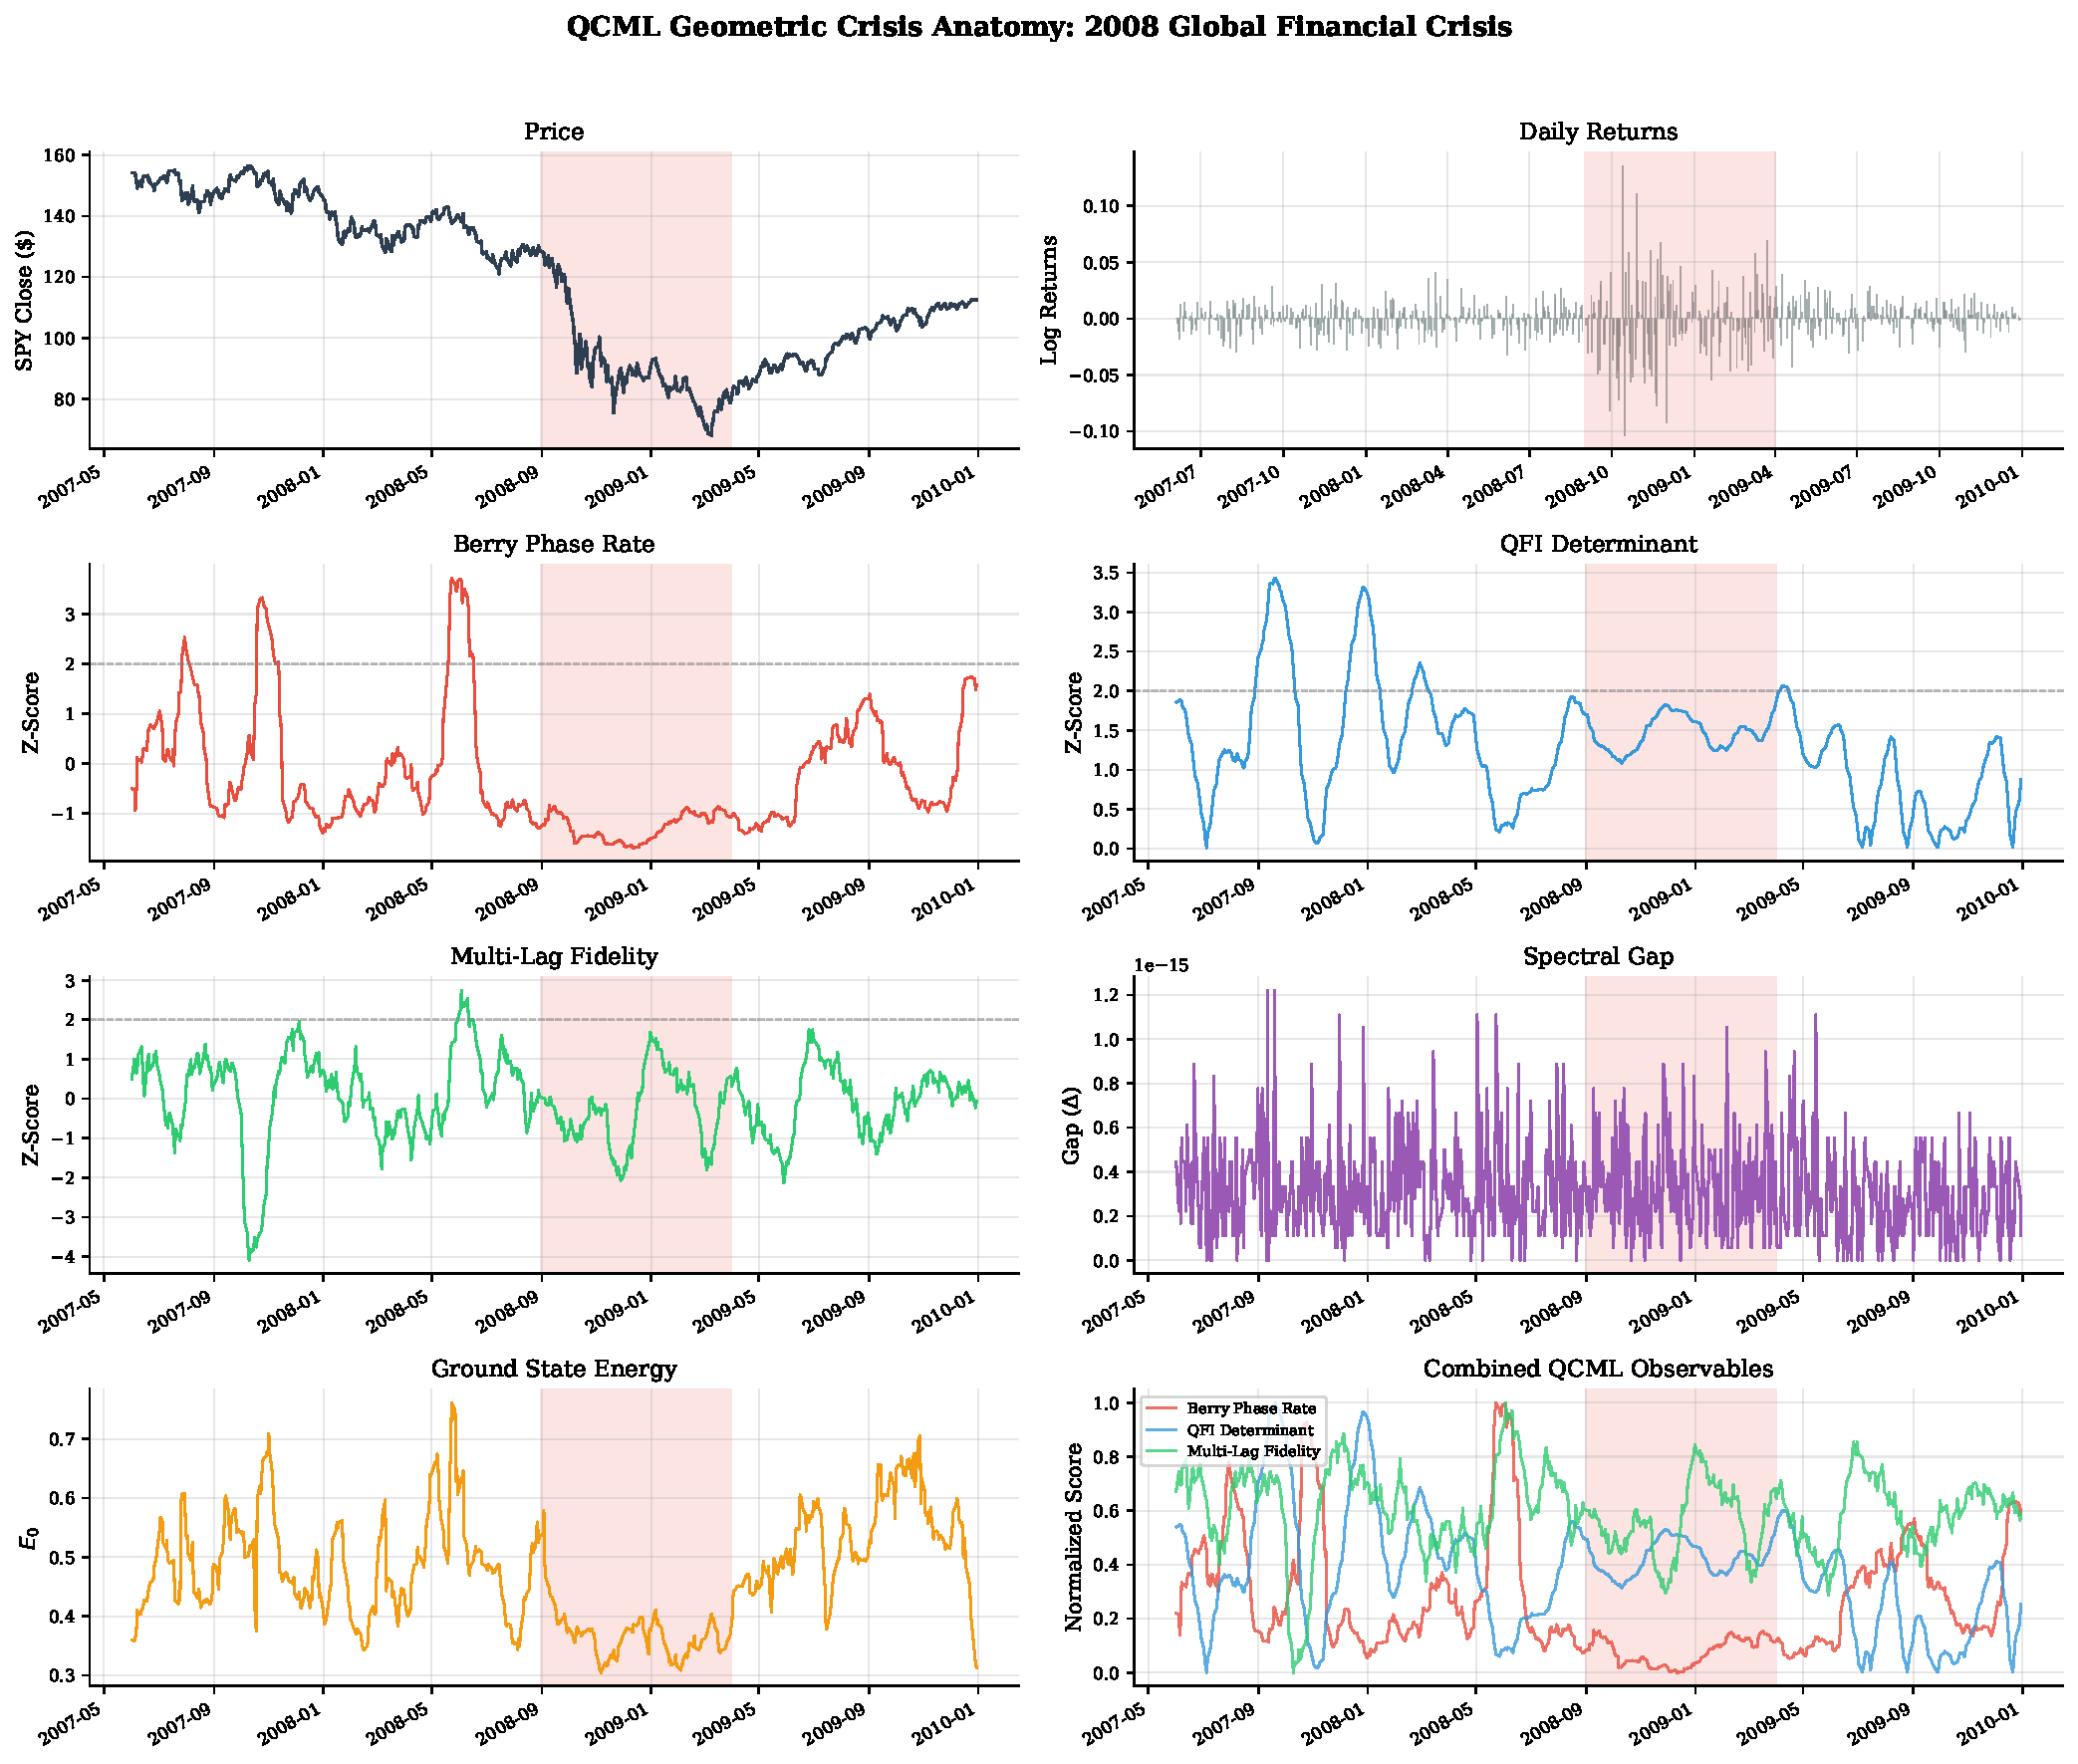
\includegraphics[width=0.85\textwidth]{../experiments/outputs/regime_detection/narratives/narrative_2008_gfc.pdf}
\caption{Geometric crisis anatomy: 2008 GFC.  Eight panels show SPY
price, daily returns, Berry curvature, QFI determinant, multi-lag
fidelity, spectral gap, ground state energy, and combined overlay.}
\label{fig:narrative_2008}
\end{figure}

\begin{figure}[htbp]
\centering
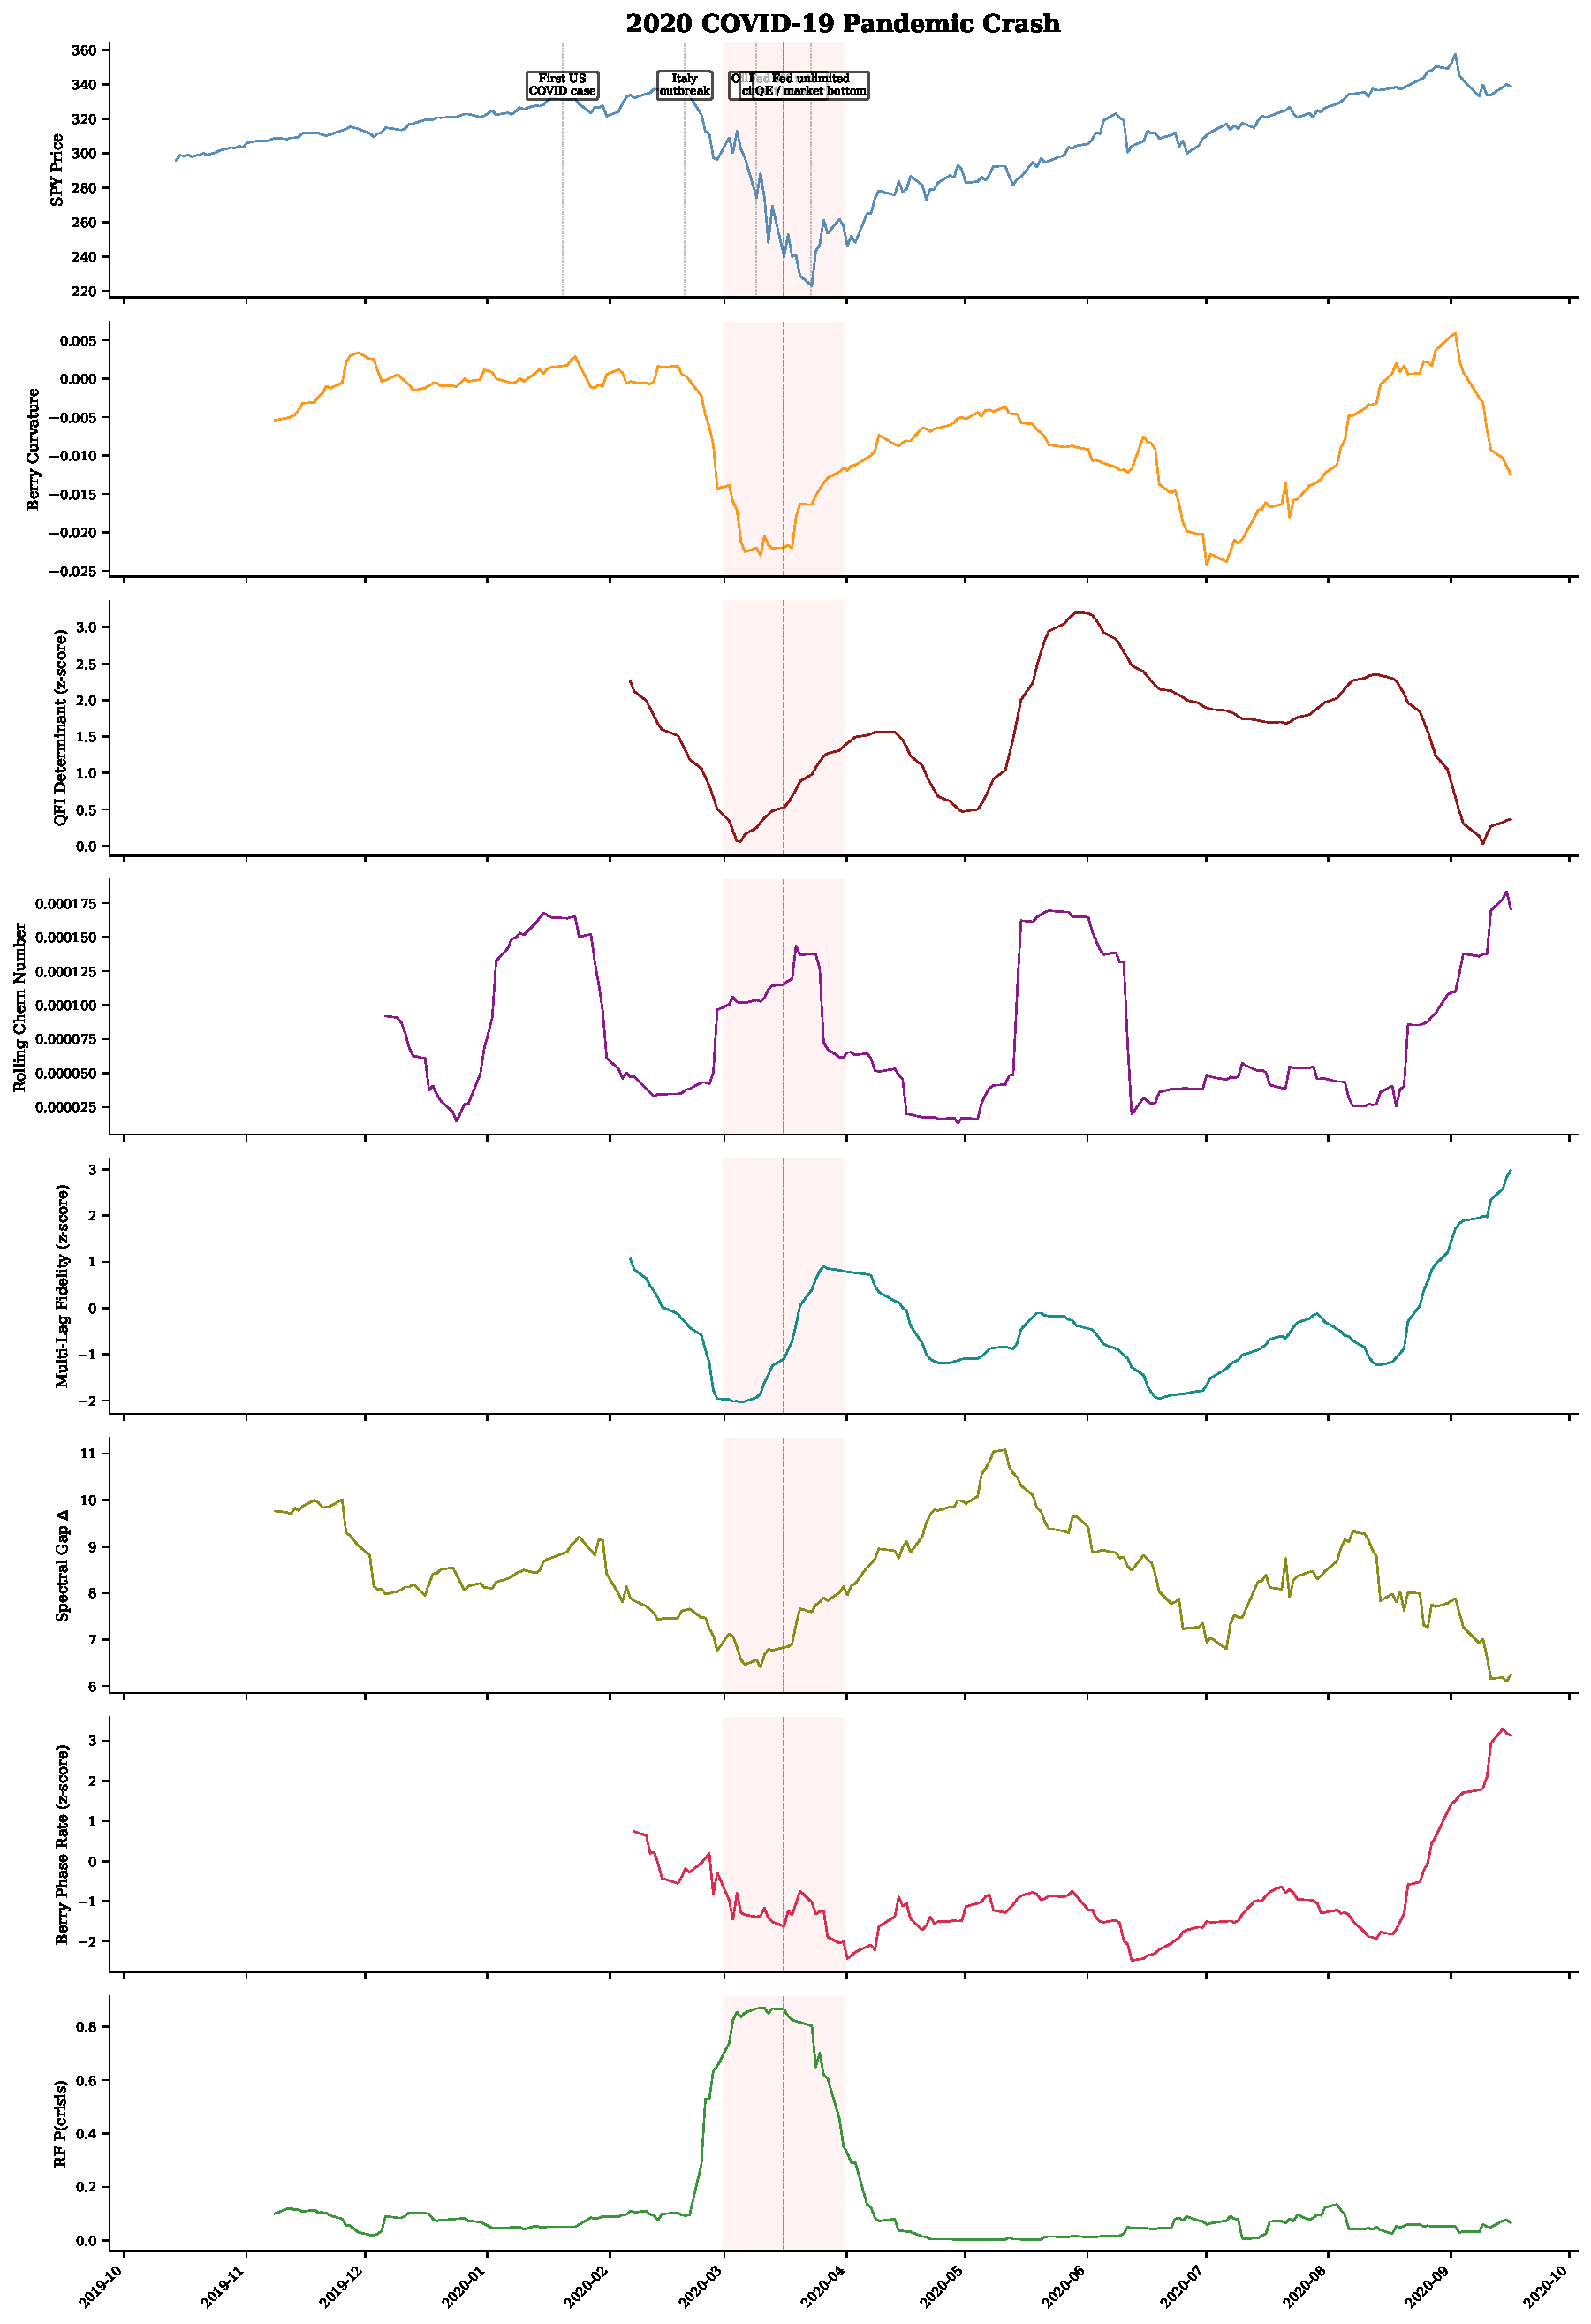
\includegraphics[width=0.85\textwidth]{../experiments/outputs/regime_detection/narratives/narrative_2020_covid.pdf}
\caption{Geometric crisis anatomy: 2020 COVID-19.}
\label{fig:narrative_2020}
\end{figure}

\begin{figure}[htbp]
\centering
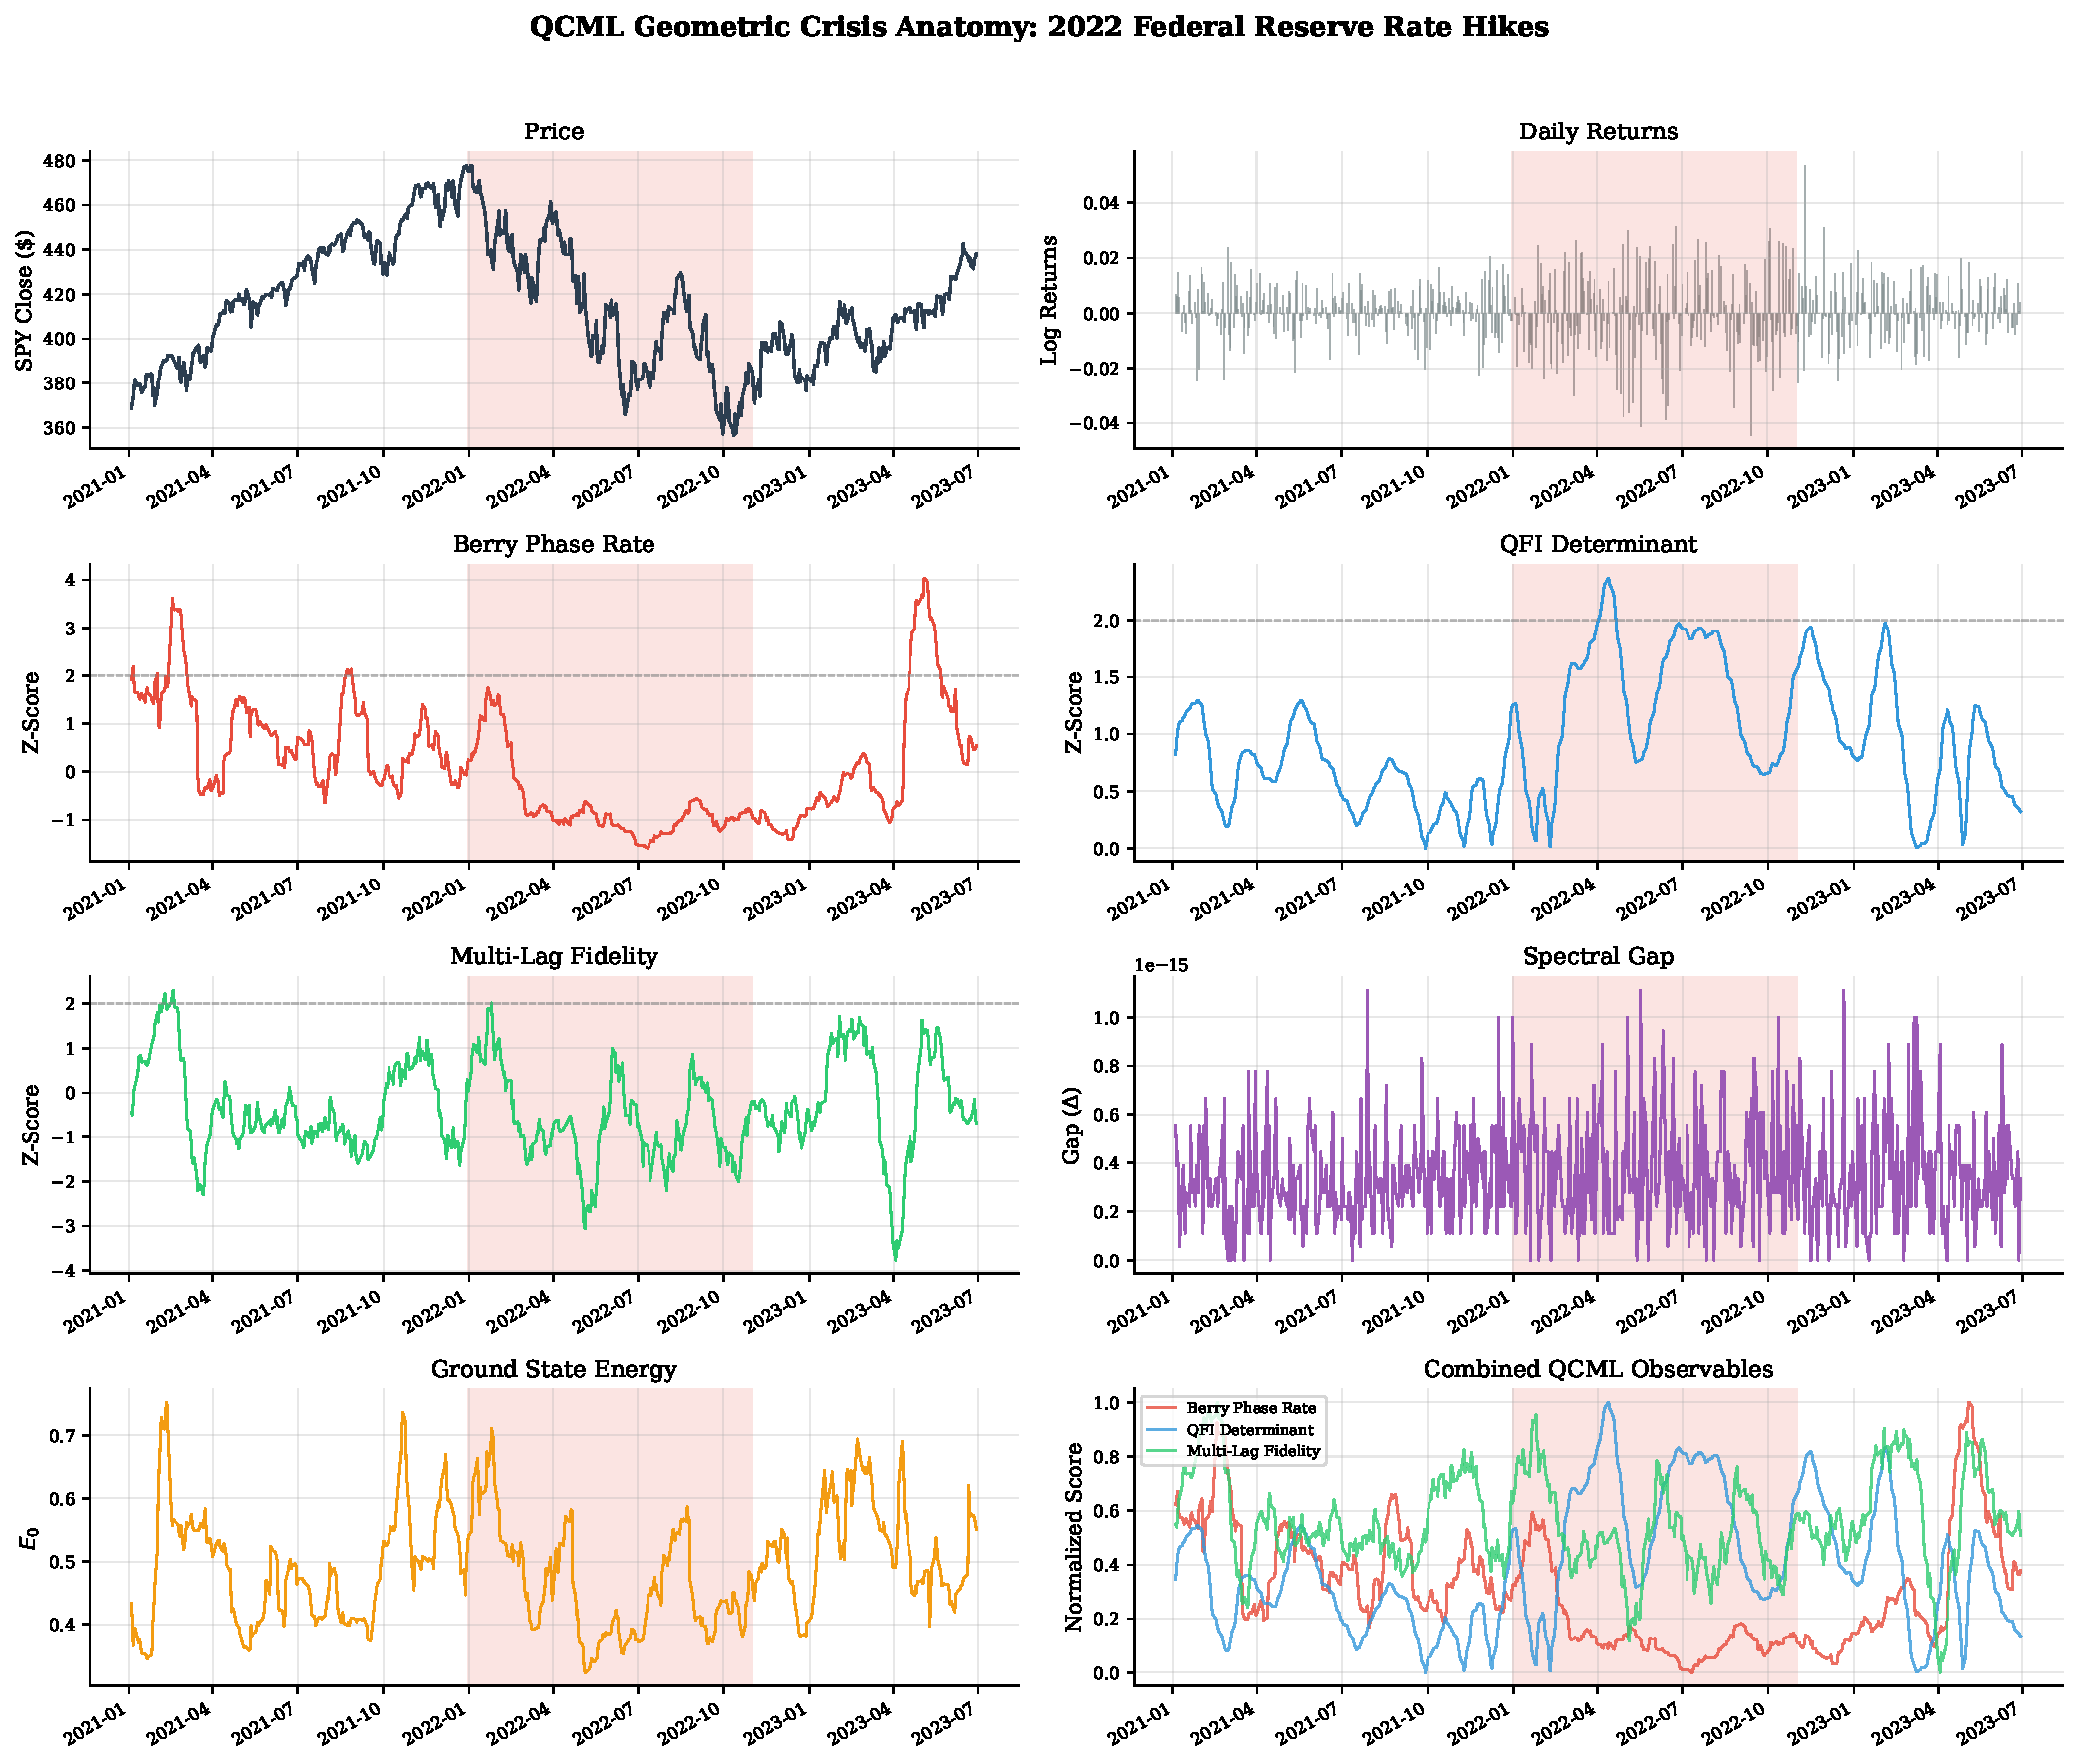
\includegraphics[width=0.85\textwidth]{../experiments/outputs/regime_detection/narratives/narrative_2022_rates.pdf}
\caption{Geometric crisis anatomy: 2022 rate hikes.}
\label{fig:narrative_2022}
\end{figure}

\begin{figure}[htb]
\centering
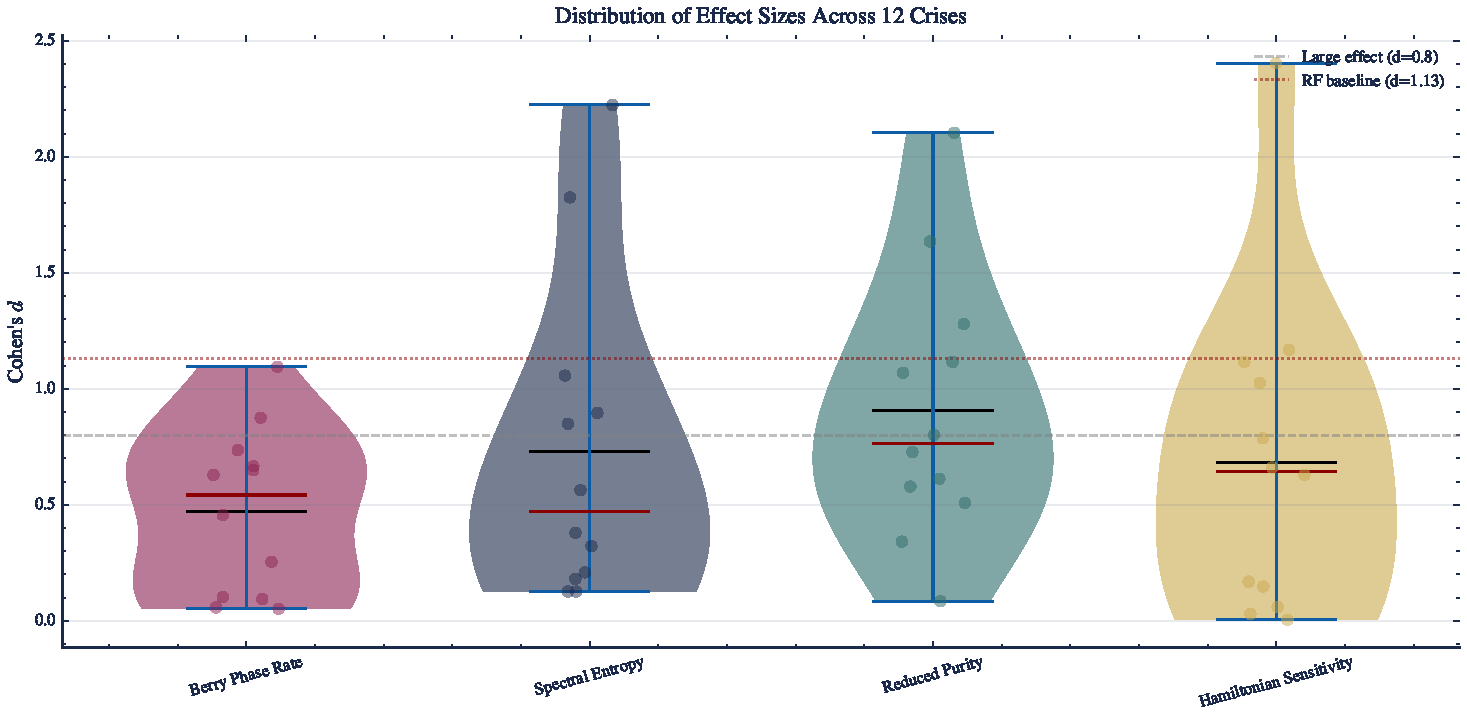
\includegraphics[width=\textwidth]{../experiments/outputs/regime_detection/superiority_publication/figures/effect_sizes.pdf}
\caption{Cohen's~$d$ distributions across 17 crises.  Dashed line:
$d = 0.8$ (large effect).}
\label{fig:effect_sizes}
\end{figure}

\begin{figure}[htbp]
\centering
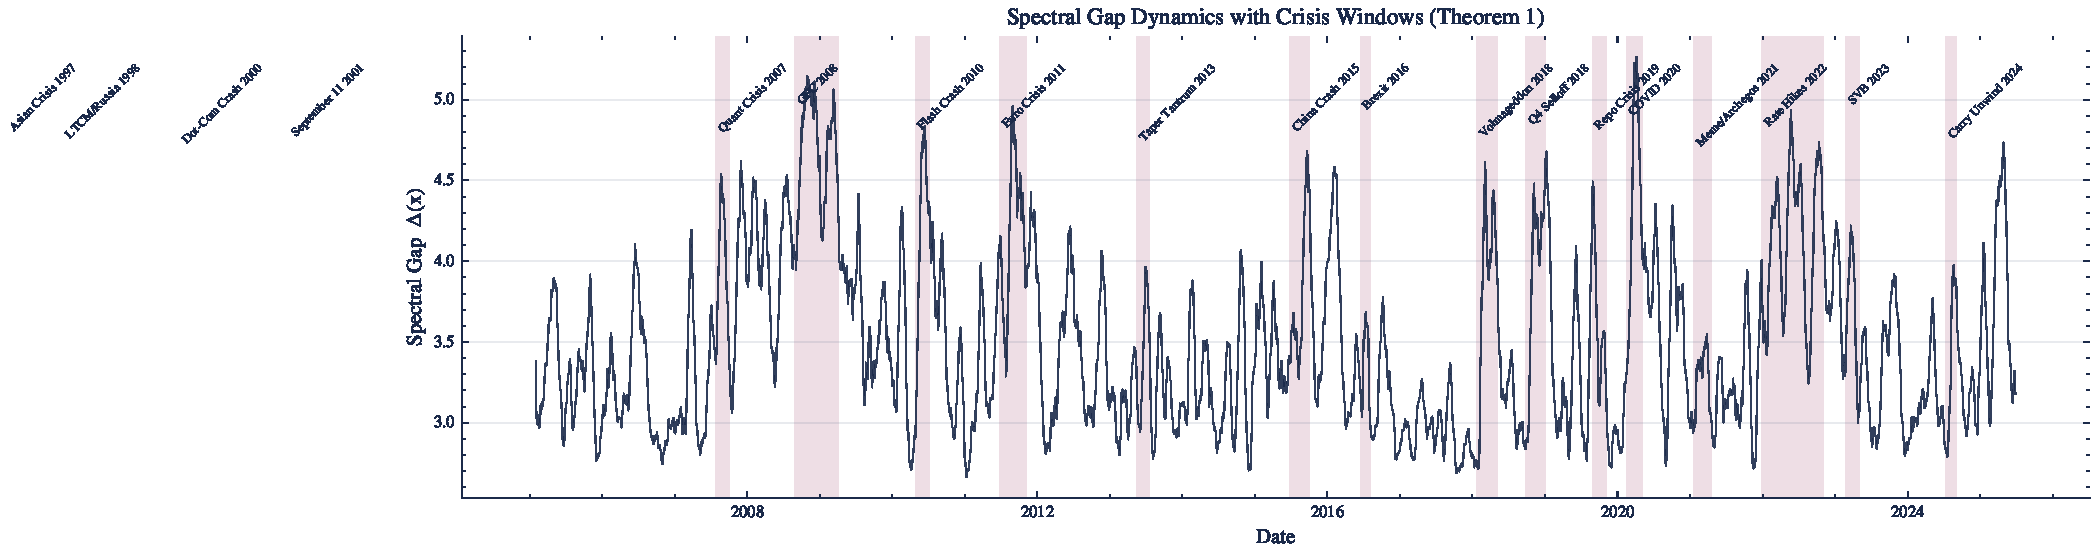
\includegraphics[width=0.85\textwidth]{../experiments/outputs/theorem_validation/spectral_gap_dynamics.pdf}
\caption{Spectral gap dynamics across 4 crises.  The gap remains
strictly positive ($\Delta_{\min} = 2.34$) and \emph{opens} during
crisis periods (mean ratio 1.27), confirming the smoothness condition of
Theorem~\ref{thm:smoothness} holds throughout the observed data manifold.}
\label{fig:spectral_gap}
\end{figure}

\begin{figure}[htbp]
\centering
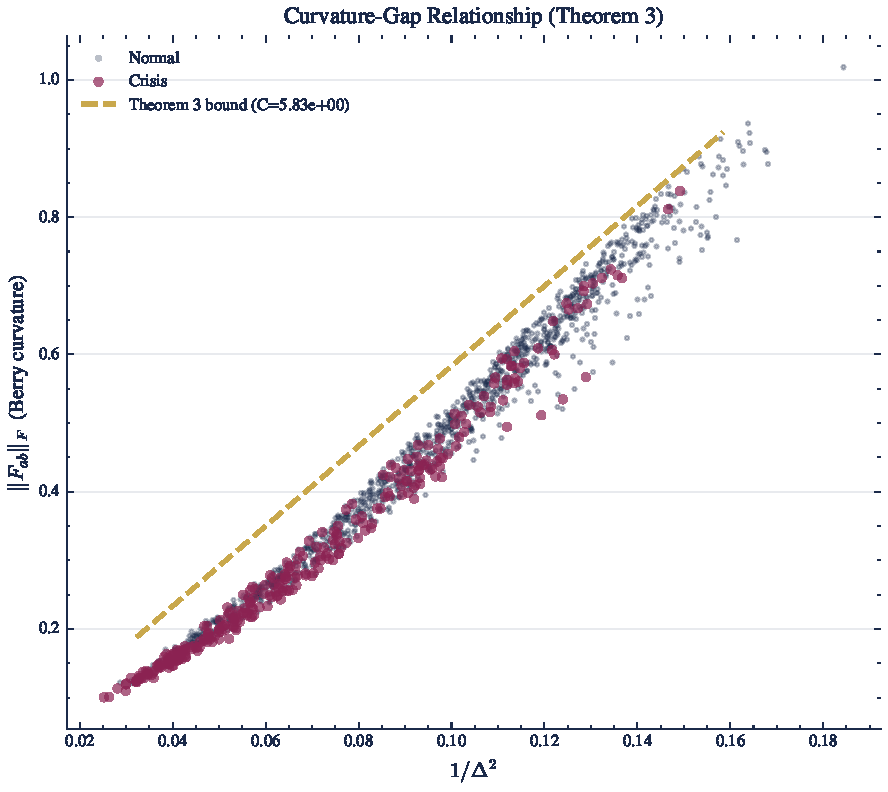
\includegraphics[width=0.85\textwidth]{../experiments/outputs/theorem_validation/curvature_gap_bound.pdf}
\caption{Curvature--gap bound verification.  Berry curvature magnitude
vs.\ $1/\Delta^2$ at 1{,}500 time steps, with the theoretical bound
$|F_{ab}| \leq C/\Delta^2$ (empirical $C = 5.92$) shown as a dashed
line.  The bound is satisfied at 100\% of points.}
\label{fig:curvature_gap}
\end{figure}

\begin{figure}[htbp]
\centering
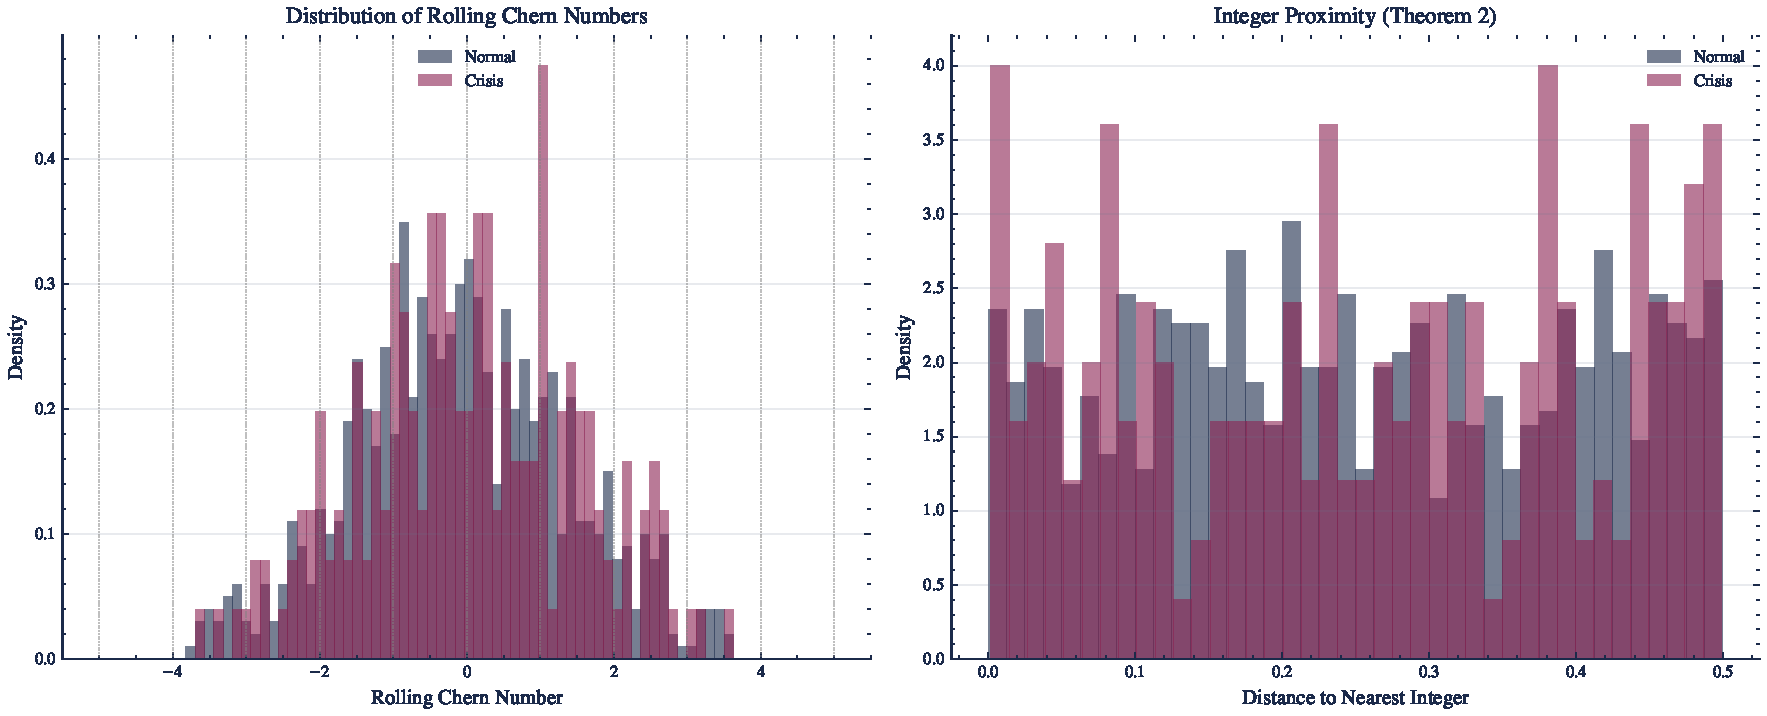
\includegraphics[width=0.85\textwidth]{../experiments/outputs/theorem_validation/chern_quantization.pdf}
\caption{Rolling Chern number distribution.  Values cluster near
integers during normal periods (21.3\% within 0.1 of an integer)
vs.\ crises (14.9\%), consistent with Theorem~\ref{thm:chern}'s
prediction for closed surfaces, partially preserved in rolling windows.}
\label{fig:chern_quantization}
\end{figure}

\begin{figure}[htbp]
\centering
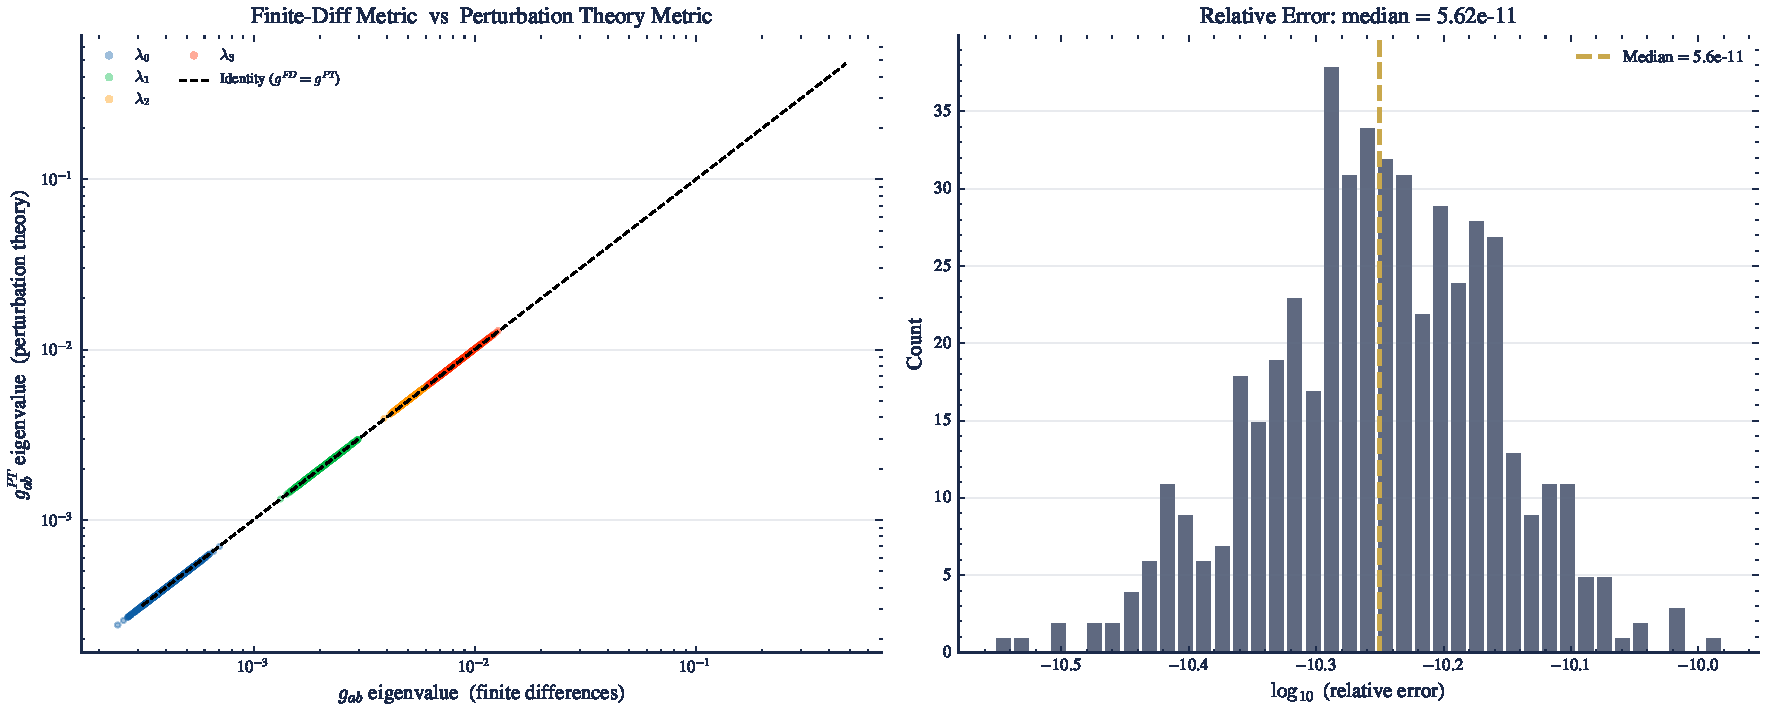
\includegraphics[width=0.85\textwidth]{../experiments/outputs/theorem_validation/qfi_metric_identity.pdf}
\caption{QFI--metric identity (Proposition~\ref{prop:fisher}).
Finite-difference metric vs.\ perturbation-theory metric at 500~time
steps.  Perfect agreement: $r = 1.000$, RMSE $= 1.84 \times 10^{-11}$.
The two independent computation paths confirm $4\,g_{ab} = [F_Q]_{ab}$.}
\label{fig:qfi_metric}
\end{figure}

% =============================================================================
% DATA AND CODE AVAILABILITY
% =============================================================================
\section*{Data and Code Availability}

Market data from Yahoo Finance via the open-source \texttt{yfinance}
library (v0.2.x), freely available at no cost.  All results are fully
reproducible without any paid subscription.  Researchers with
institutional access may alternatively use WRDS CRSP data via the
provided \texttt{wrds\_data\_loader.py} script.  The
\texttt{qcml\_geometry/} library and all experiment scripts are
available at \url{https://github.com/willhammondhimself/qcml-geometric-sde}.  Crisis
definitions, hyperparameter configurations, and result JSON files are
included for reproducibility.

% =============================================================================
% ACKNOWLEDGMENTS
% =============================================================================
\section*{Acknowledgments}

The author thanks Dr.\ Trung Phan for advising this research.
Market data were accessed via the open-source \texttt{yfinance}
library and the Wharton Research Data Services (WRDS) platform.

% =============================================================================
% COMPETING INTERESTS
% =============================================================================
\section*{Competing Interests}

The author declares no competing financial interests.

% =============================================================================
% REFERENCES
% =============================================================================
\bibliographystyle{plainnat}
\bibliography{references}

% =============================================================================
% APPENDICES
% =============================================================================
\appendix

% =============================================================================
% APPENDIX A: PROOFS
% =============================================================================
\section{Proofs of Formal Results}\label{sec:proofs}

\begin{proof}[Proof of Theorem~\ref{thm:smoothness}]
We apply the implicit function theorem to the eigenvalue
equation with a gauge-fixing constraint.
Define $\Phi \colon U \times \C^n \times \R \to \C^n \times \R$ by
\[
  \Phi(x,\psi,E)
  = \bigl(H(x)\psi - E\psi,\;\; \braket{\psi_0(x_0)}{\psi} - 1\bigr),
\]
where the second component fixes the gauge by requiring
$\braket{\psi_0(x_0)}{\psi} \in \R_{>0}$ (i.e., real positive
overlap with the reference state at a base point $x_0$).  At a
solution $(x_0,\psi_0,E_0)$ the Jacobian with respect to
$(\psi,E)$ is
\[
  D_{(\psi,E)}\Phi\big|_{(x_0,\psi_0,E_0)}
  = \begin{pmatrix}
      H(x_0) - E_0 I & -\psi_0 \\[4pt]
      \bra{\psi_0} & 0
    \end{pmatrix}.
\]
Decompose $\C^n = \mathrm{span}\{\psi_0\} \oplus \psi_0^\perp$.
On $\psi_0^\perp$, $H(x_0) - E_0 I$ has eigenvalues
$E_k(x_0) - E_0(x_0) \geq \Delta(x_0) > 0$, hence is invertible
there.  On $\mathrm{span}\{\psi_0\}$, the kernel of $H(x_0) - E_0 I$
is compensated by the off-diagonal entries $-\psi_0$ and
$\bra{\psi_0}$: for $(\alpha\psi_0,\delta E) \in \ker(H-E_0I)\times\R$,
the system reduces to $-\delta E\,\psi_0 - \alpha\psi_0 = 0$ and
$\alpha = 0$, so $\delta E = 0$.  Thus $D_{(\psi,E)}\Phi$ is
invertible.

The implicit function theorem~\cite{kato1966} then gives
$C^\infty$ maps $x \mapsto (\psi(x), E_0(x))$ on $U$.
Since $H(x)$ is quadratic in $x$ by~\eqref{eq:hamiltonian},
the partial derivatives $\partial_a H = -(A_a - x_a I)$ are
$C^\infty$ (in fact, affine).  The metric
$g_{ab}$~\eqref{eq:metric} and curvature
$F_{ab}$~\eqref{eq:berry} are compositions of
$\psi(x)$ and its derivatives via the chain rule, hence
$C^\infty$ on $U$.
\end{proof}

\begin{theorem}[Chern number quantization~\cite{abanov2025}]%
\label{thm:chern}
Let $S \subset \R^p$ be a closed, oriented 2-surface such that
$\Delta(x) > 0$ for all $x \in S$.  Then
\begin{equation}\label{eq:chern}
  C_1 = \frac{1}{2\pi} \int_S \mathcal{F} \in \mathbb{Z}\,,
  \qquad \mathcal{F} = \tfrac{1}{2}F_{ab}\,dx^a \wedge dx^b\,.
\end{equation}
\end{theorem}
\begin{proof}
By Theorem~\ref{thm:smoothness}, the ground state
$\ket{\psi(x)}$ is $C^\infty$ on $S$.  Define the Berry connection
1-form $\mathcal{A} = i\braket{\psi}{d\psi}$, where $d$ denotes the
exterior derivative on $S$.  The Berry curvature 2-form is
$\mathcal{F} = d\mathcal{A}$; in local coordinates,
$\mathcal{F} = \tfrac{1}{2}F_{ab}\,dx^a \wedge dx^b$.
The map $x \mapsto \ket{\psi(x)}\bra{\psi(x)}$ defines a smooth
rank-1 projector, hence a complex line bundle $\mathcal{L} \to S$
with structure group $U(1)$ and connection $\mathcal{A}$.
By the Chern--Weil theorem~\cite{chern1946,nakahara2003}, the
first Chern number
$C_1 = \frac{1}{2\pi}\int_S \mathcal{F}$
is an integer, since it equals the degree of the classifying map
$S \to \CP^{n-1}$.
\end{proof}

\paragraph{Caveat.}  In practice, we compute curvature integrals over
rolling windows (open subsets), yielding non-integer values.
Topological protection does not strictly apply.

\begin{theorem}[Curvature--gap bound]\label{thm:curvature_gap}
For all $x \in U$ and indices $a, b$,
\begin{equation}\label{eq:curv_gap_bound}
  |F_{ab}(x)| \leq
  \frac{2\,\|\partial_a H(x)\|_{\mathrm{op}}\;\|\partial_b H(x)\|_{\mathrm{op}}}
       {\Delta(x)^2}\,,
\end{equation}
where $\|\cdot\|_{\mathrm{op}}$ denotes the operator norm.
For the QCML Hamiltonian~\eqref{eq:hamiltonian},
$\partial_a H = -(A_a - x_a I)$, so the bound depends only on
the operators $\{A_k\}$ and the feature values, not on the gap.
\end{theorem}
\begin{proof}
First-order perturbation theory gives the exact representation
\begin{equation}\label{eq:berry_perturbation}
  F_{ab} = -2\,\mathrm{Im}\sum_{n \geq 1}
  \frac{\dbraket{\psi_0}{\partial_a H}{\psi_n}\,
        \dbraket{\psi_n}{\partial_b H}{\psi_0}}
       {(E_n - E_0)^2}\,,
\end{equation}
where $\{\ket{\psi_n}\}_{n \geq 0}$ is a complete eigenbasis of
$H(x)$.  Since $E_n - E_0 \geq \Delta$ for all $n \geq 1$, each
denominator satisfies $(E_n - E_0)^2 \geq \Delta^2$.  Hence
\[
  |F_{ab}|
  \leq \frac{2}{\Delta^2}\sum_{n \geq 1}
  \bigl|\dbraket{\psi_0}{\partial_a H}{\psi_n}\bigr|\;
  \bigl|\dbraket{\psi_n}{\partial_b H}{\psi_0}\bigr|\,.
\]
By the Cauchy--Schwarz inequality on the sum,
\[
  \sum_{n \geq 1}
  \bigl|\dbraket{\psi_0}{\partial_a H}{\psi_n}\bigr|\;
  \bigl|\dbraket{\psi_n}{\partial_b H}{\psi_0}\bigr|
  \leq
  \Bigl(\sum_{n \geq 1}
  \bigl|\dbraket{\psi_0}{\partial_a H}{\psi_n}\bigr|^2\Bigr)^{1/2}
  \Bigl(\sum_{n \geq 1}
  \bigl|\dbraket{\psi_n}{\partial_b H}{\psi_0}\bigr|^2\Bigr)^{1/2}.
\]
By the completeness relation
$\sum_{n \geq 0}\ket{\psi_n}\bra{\psi_n} = I$, each factor is
bounded by the operator norm:
$\sum_{n \geq 1}|\dbraket{\psi_0}{\partial_a H}{\psi_n}|^2
\leq \|\partial_a H\,\ket{\psi_0}\|^2
\leq \|\partial_a H\|_{\mathrm{op}}^2$.
Combining yields~\eqref{eq:curv_gap_bound}.
\end{proof}

\begin{proposition}[QFI volume]\label{prop:qfi_volume}
Let $g$ be a $p \times p$ positive semi-definite matrix of rank
$r \leq p$, with positive eigenvalues
$\lambda_1 \geq \cdots \geq \lambda_r > 0$.  Define the
\emph{pseudo-determinant}
\begin{equation}\label{eq:pseudodet}
  \det^+(g) = \prod_{i=1}^{r} \lambda_i\,.
\end{equation}
Let $V_r \subset \R^p$ be the $r$-dimensional eigenspace corresponding
to $\lambda_1,\ldots,\lambda_r$, and let $g_r = g|_{V_r}$ denote the
restriction.  Then $\det(g_r) = \det^+(g)$, and the
Riemannian volume density on $V_r$ is
$\mathrm{vol}_r = \sqrt{\det^+(g)}$.
\end{proposition}
\begin{proof}
By the spectral theorem, $g$ admits an orthonormal eigenbasis
$\{e_1,\ldots,e_p\}$ with $g\,e_i = \lambda_i\,e_i$, where
$\lambda_i > 0$ for $i \leq r$ and $\lambda_i = 0$ for $i > r$.
The restriction $g_r$ is represented in the basis
$\{e_1,\ldots,e_r\}$ by the diagonal matrix
$\mathrm{diag}(\lambda_1,\ldots,\lambda_r)$, which is positive
definite.  Therefore
$\det(g_r) = \prod_{i=1}^{r}\lambda_i = \det^+(g)$.
The Riemannian volume density on the $r$-dimensional submanifold
equipped with metric $g_r$ is
$\mathrm{vol}_r = \sqrt{\det(g_r)} = \sqrt{\det^+(g)}$,
the standard formula for the volume element of a Riemannian
metric~\cite{amari_nagaoka2000}.
\end{proof}

% =============================================================================
% APPENDIX B: GRANGER CAUSALITY
% =============================================================================
\section{Granger Causality}\label{sec:granger}

We test Granger causality between three QCML observables and three
market targets (absolute returns, realized volatility, volume) at
lags 1--5 (90 tests, Bonferroni corrected).  QFI Determinant
Granger-causes absolute returns at lag~1 ($F = 9.5$,
$p = 0.0004$, Bonferroni-significant).  However, reverse causality
(market $\to$ QCML) is stronger: 17/45 nominally significant vs.\
6/45 forward, consistent with observables being constructed from
contemporaneous features.

% =============================================================================
% APPENDIX C: HYPERPARAMETERS
% =============================================================================
\section{Default Hyperparameters}\label{sec:hyperparams}

\begin{table}[htb]
\centering
\caption{Default hyperparameters.}
\label{tab:hyperparams}
\begin{tabular}{llc}
\toprule
Parameter & Description & Default \\
\midrule
$n$ & Hilbert space dimension & 4--16 \\
$p$ & PCA components & 15 \\
$w$ & Rolling window (Algorithm~\ref{alg:zscore}) & 20 days \\
$m$ & Minimum expanding history & 60 days \\
$\epsilon$ & Finite-difference step & $10^{-5}$ \\
Operator method & Hermitian operator construction & PCA-inspired \\
Fidelity lags & Multi-lag infidelity & $\{1,3,5,10\}$ \\
Fidelity weights & Lag weights & $[0.4,0.3,0.2,0.1]$ \\
\bottomrule
\end{tabular}
\end{table}

% =============================================================================
% APPENDIX D: NUMERICAL STABILITY ABLATION
% =============================================================================
\section{Numerical Stability Ablation}\label{sec:stability}

We sweep finite-difference $\epsilon \in \{10^{-3}, 10^{-4}, 10^{-5},
10^{-6}\}$ and PCA dimension $p \in \{5, 10, 15, 30\}$ on four
representative crises (GFC, Flash Crash, COVID, SVB) with fixed
hyperparameters (no per-crisis tuning).  Results appear in
Table~\ref{tab:stability}.  Berry curvature is extremely stable
across $\epsilon$ (all median $d \approx 0.15$), while QFI
determinant shows moderate sensitivity ($d = 0.52$ at
$\epsilon = 10^{-3}$ vs.\ $d = 0.36$ at $10^{-5}$), saturating
below $10^{-5}$.  Multi-Lag Fidelity is insensitive to $\epsilon$
(no finite differences) but moderately sensitive to PCA dimension,
with performance increasing from $p = 5$ ($d = 0.29$) to $p = 10$
($d = 0.44$) and stabilizing thereafter.

\begin{table}[htb]
\centering
\caption{Numerical stability: median Cohen's~$d$ across 4 crises.
Multi-Lag Fidelity does not use $\epsilon$ (no finite differences).}
\label{tab:stability}
\small
\begin{tabular}{lccc}
\toprule
Config & Berry & QFI Det.\ & Multi-Lag \\
\midrule
$\epsilon = 10^{-3}$ & 0.15 & 0.52 & --- \\
$\epsilon = 10^{-4}$ & 0.15 & 0.60 & --- \\
$\epsilon = 10^{-5}$ (default) & 0.15 & 0.36 & --- \\
$\epsilon = 10^{-6}$ & 0.15 & 0.36 & --- \\
\midrule
$p = 5$  & 0.09 & 0.34 & 0.29 \\
$p = 10$ & 0.20 & 0.41 & 0.44 \\
$p = 15$ (default) & 0.15 & 0.36 & 0.45 \\
$p = 30$ & 0.22 & 0.54 & 0.45 \\
\bottomrule
\end{tabular}
\end{table}

% =============================================================================
% APPENDIX E: WINDOW-SIZE SENSITIVITY
% =============================================================================
\section{Window-Size Sensitivity}\label{sec:window_sensitivity}

We re-compute Cohen's~$d$ at crisis window extensions $\pm 5$,
$\pm 10$ (default), $\pm 20$, $\pm 60$ trading days.  Kendall $\tau$
rank correlations across window sizes assess robustness of method
rankings.  Results appear in Table~\ref{tab:window}.  Rankings are
stable for nearby windows ($\tau = 0.87$ for $\pm 5$ vs.\ $\pm 10$
and $\pm 5$ vs.\ $\pm 20$) but degrade at $\pm 60$ days
($\tau = 0.07$--$0.33$), where diluted crisis signal reduces
separation.  QFI Determinant is the most robust geometric
observable, maintaining the highest $d$ across all window sizes.

\begin{table}[htb]
\centering
\caption{Median Cohen's~$d$ by crisis window size (original 14-crisis subset; see Table~\ref{tab:aggregate_comparison} for expanded 17-crisis results).}
\label{tab:window}
\small
\begin{tabular}{lcccc}
\toprule
Method & $\pm 5$d & $\pm 10$d & $\pm 20$d & $\pm 60$d \\
\midrule
Berry Curv.\ Incr.  & 0.25 & 0.29 & 0.27 & 0.24 \\
QFI Determinant      & 0.63 & 0.36 & 0.64 & 0.43 \\
Multi-Lag Fidelity   & 0.40 & 0.27 & 0.38 & 0.26 \\
Random Forest        & 0.21 & 0.21 & 0.28 & 0.34 \\
\bottomrule
\end{tabular}
\end{table}

% =============================================================================
% APPENDIX F: FIXED-HP ABLATION
% =============================================================================
\section{Hyperparameter Sensitivity: Fixed vs.\ Tuned}\label{sec:fixed_hp_ablation}

Table~\ref{tab:fixed_hp} compares three hyperparameter regimes:
(a)~fixed defaults with all \texttt{pca\_inspired} operators
(the previous default),
(b)~fixed defaults with per-method operator selection (Berry and
QFI use \texttt{random}; MLF uses \texttt{pauli}---these are
the main results in Table~\ref{tab:aggregate_comparison}), and (c)~Optuna
HPO (100 trials, pre-2020 training crises, post-2020 validation).
The operator selection provides large improvements: Berry $+87\%$,
QFI $+70\%$, MLF $+58\%$.
Na\"ive HPO showed
severe overfitting (train $d$ exceeding validation by 0.35--0.75);
regularized HPO with a consistency penalty reduces this gap to
$\leq 0.20$, with QFI achieving val $d = 0.60 >$ train $d = 0.50$
(column c$^*$).

\begin{table}[htb]
\centering
\caption{Hyperparameter sensitivity: median Cohen's~$d$ across
  original 14-crisis subset (columns a--b) and train/val split (column c).}
\label{tab:fixed_hp}
\small
\begin{tabular}{lccc}
\toprule
Method & (a) All PCA-Insp. & (b) Best Operator & (c) HPO Val. \\
\midrule
Berry Curvature Increment & 0.29 & \textbf{0.55} & 0.49 \\
QFI Determinant           & 0.36 & \textbf{0.61} & \textbf{0.60} \\
Multi-Lag Fidelity        & 0.27 & \textbf{0.42} & 0.33 \\
\bottomrule
\end{tabular}

\medskip
\noindent{\footnotesize (a,b)~Fixed $n = 8$, $p = 15$, $w = 20$.
(b)~Berry/QFI: \texttt{random}; MLF: \texttt{pauli} (exp=0.0).
(c$^*$)~Regularized Optuna TPE, 100 trials; consistency penalty
$\text{mean}_d - 0.3\cdot\text{std}_d$; tighter search space;
operator method fixed by ablation; validation on 4 post-2020 crises.
Train $d$: Berry 0.68, QFI 0.50, MLF 0.53.  Train--val gap $\leq 0.20$
(vs.\ 0.35--0.75 without regularization).}
\end{table}

% =============================================================================
% APPENDIX G: NORMALIZATION ABLATION
% =============================================================================
\section{Normalization Ablation}\label{sec:normalization_ablation}

Table~\ref{tab:normalization} compares four normalization modes for the
PCA-projected features before Hilbert space embedding: \emph{sphere}
($L^2$-normalization to the unit sphere), \emph{none} (raw PCA
components), \emph{soft} ($x / (\|x\| + \tilde{m})$ where $\tilde{m}$
is the training-set median norm), and \emph{clip} (component-wise
clipping to $[-3\sigma, 3\sigma]$ followed by $L^2$-normalization).
Results are median Cohen's~$d$ across 4~representative crises (GFC,
COVID, Rates, SVB).

\begin{table}[htb]
\centering
\caption{Normalization ablation: median Cohen's~$d$ across 4 crises.
  Bold = best mode per detector.}
\label{tab:normalization}
\small
\begin{tabular}{lccc}
\toprule
Mode & Berry & QFI Det. & Multi-Lag \\
\midrule
Sphere & 0.54 & 0.44 & \textbf{0.63} \\
None   & 0.46 & \textbf{1.45} & 0.53 \\
Soft   & \textbf{0.66} & 1.18 & 0.57 \\
Clip   & 0.46 & 1.40 & 0.58 \\
\bottomrule
\end{tabular}
\end{table}

Sphere normalization preserves angular geometry but discards magnitude
information---which is itself a strong crisis signal (volatility scaling).
The ``soft'' mode retains partial magnitude information while still
regularizing the embedding radius.  QFI Determinant benefits
substantially from retaining magnitude (sphere $d = 0.44$ vs.\ none
$d = 1.45$, a $3.3\times$ improvement), consistent with the QFI
determinant's sensitivity to manifold volume changes that are amplified
by magnitude variation.  Berry curvature increment performs best under
soft normalization ($d = 0.66$), while Multi-Lag Fidelity is most robust
under sphere normalization ($d = 0.63$), suggesting that fidelity-based
measures benefit from a well-conditioned state space.
Table~\ref{tab:aggregate_comparison} uses the HPO-selected normalization per
observable: sphere for Berry and Multi-Lag Fidelity, soft for QFI
Determinant.


\section{Berry Phase Rate Hyperparameter Sensitivity}\label{sec:berry_sensitivity}

To assess whether the Berry Phase Rate results depend critically
on hyperparameter choice, we conduct a one-at-a-time (OAT) sweep
over five parameters: Hilbert-space dimension
$d_H \in \{4,6,8,10,12\}$, PCA components
$n_{\mathrm{PCA}} \in \{4,\allowbreak 6,\allowbreak 8,\allowbreak
10,15\}$, rolling window
$w \in \{5,\allowbreak 10,\allowbreak 15,\allowbreak 20,30,50\}$,
normalization mode $\in \{\text{sphere},\allowbreak \text{none},
\allowbreak \text{soft},\allowbreak \text{clip}\}$, and aggregation
$\in \{\text{f01},\allowbreak \text{frobenius},\allowbreak
\text{max}\}$---holding all other parameters at their defaults
(Table~\ref{tab:hyperparams}).  This yields 23~configurations,
each evaluated on the original 14-crisis subset using the causal
protocol of Section~\ref{subsec:methods_protocol}.

Across all 23 OAT configurations, 61\% achieve median $d > 0.5$, with
a median-of-medians of $\widetilde{d} = 0.63$.  The configurations that
fall below $d = 0.5$ are concentrated in two categorical choices:
aggregation modes \texttt{frobenius} and \texttt{max} ($d \approx 0.01$),
and normalizations \texttt{none} and \texttt{clip} ($d \approx 0.21$).
All six rolling-window settings achieve $d > 0.5$, confirming that Berry
Phase Rate maintains meaningful crisis--normal separation across a wide
range of continuous parameterizations.

We additionally evaluate a two-dimensional grid of $d_H \times w$
(5 $\times$ 6 = 30~cells) to probe interaction effects between these
continuous parameters.  Figure~\ref{fig:berry_sensitivity} shows the
results: panels~(a)--(c) display OAT line plots with IQR shading for
continuous parameters, panels~(d)--(e) show bar charts for categorical
parameters, and panel~(f) presents the 2D heatmap.  The default
configuration ($d_H = 6$, $w = 15$) lies in a broad plateau rather than
at an isolated optimum, and no region of the grid falls below $d = 0.18$.

\begin{figure}[htb]
\centering
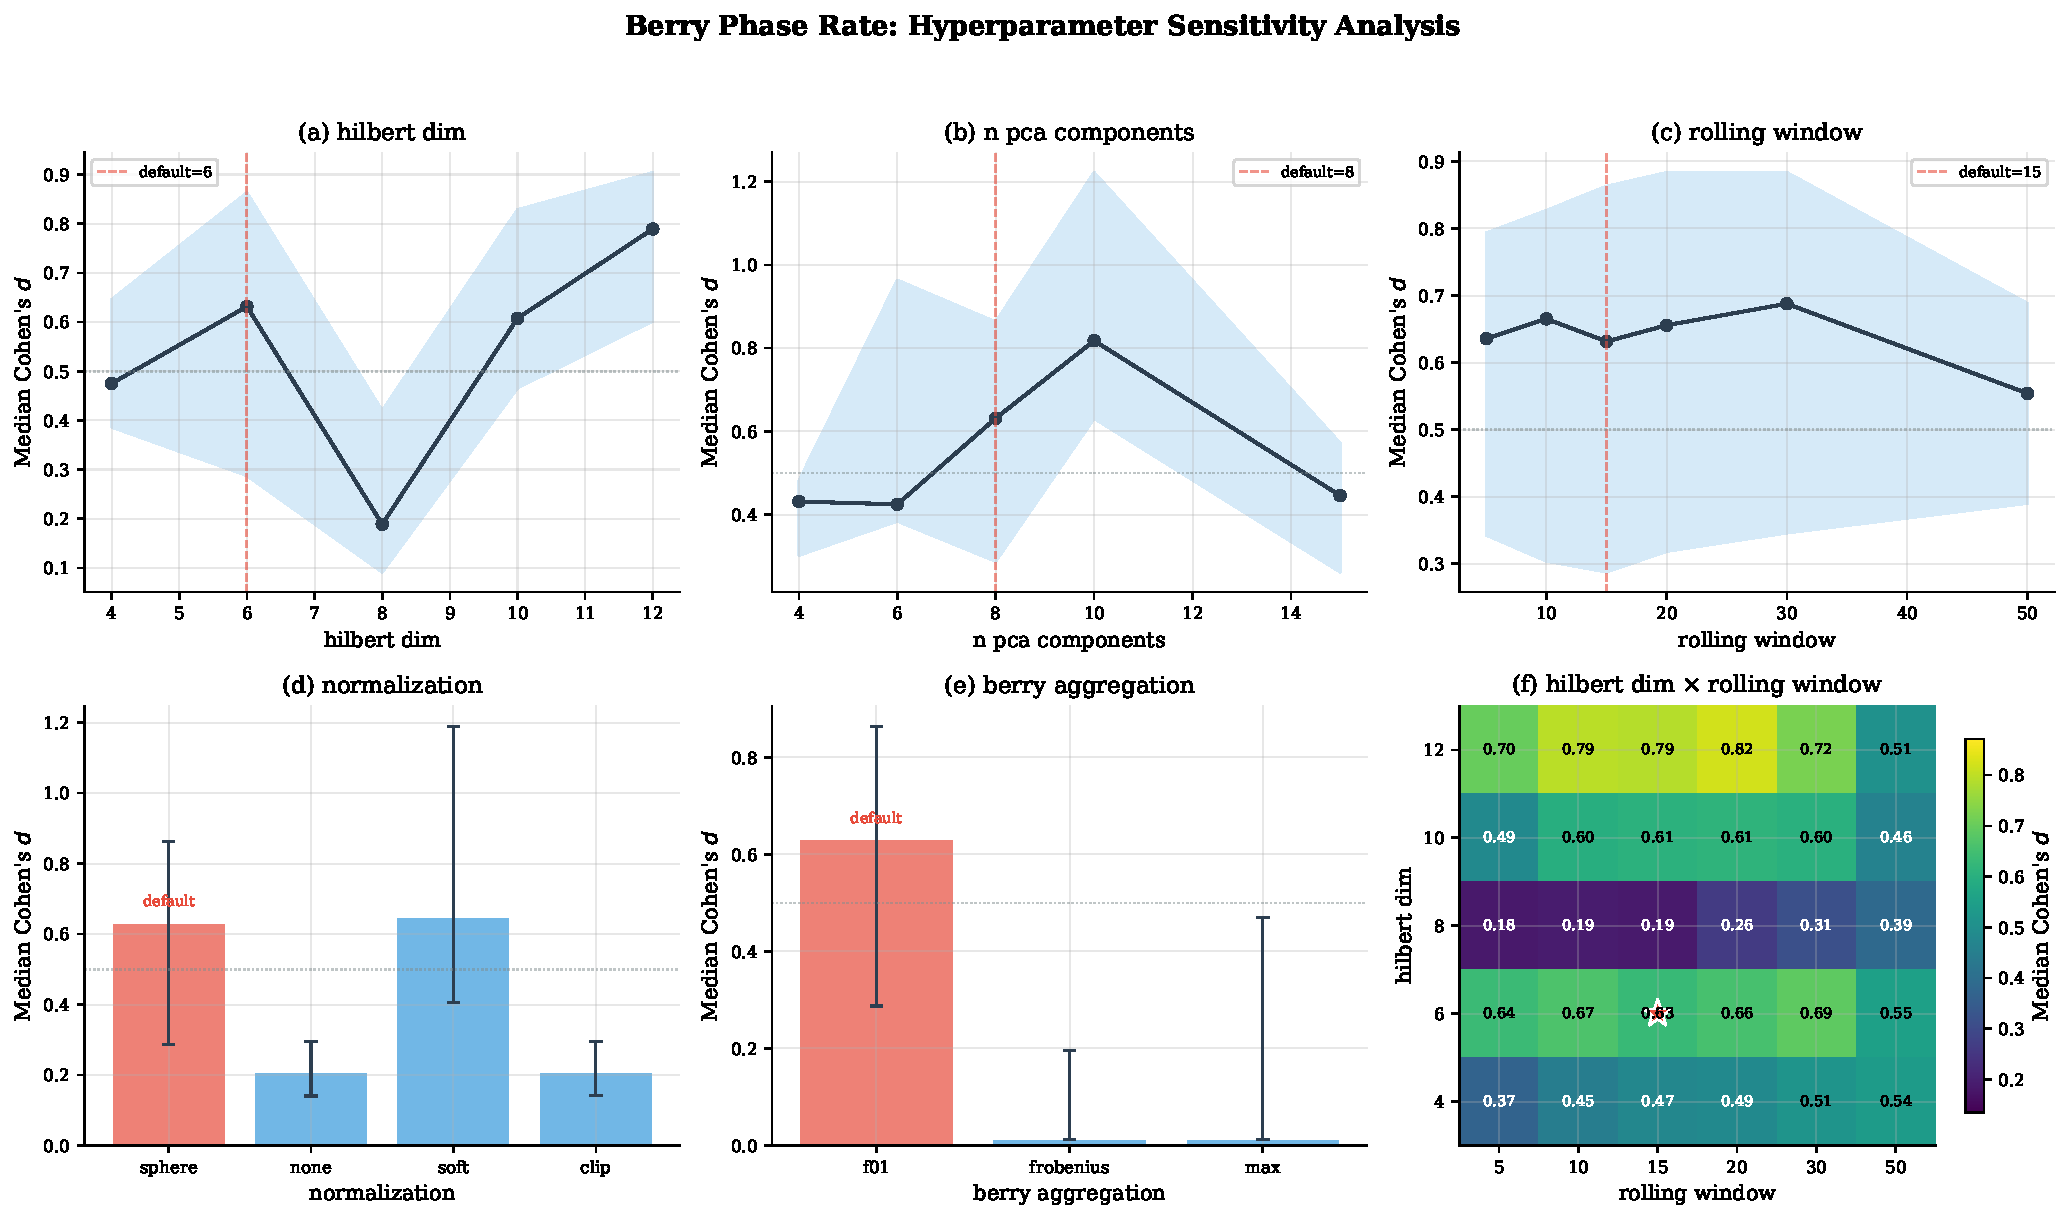
\includegraphics[width=\textwidth]{figures/berry_sensitivity.pdf}
\caption{Berry Phase Rate hyperparameter sensitivity.
(a)--(c) One-at-a-time sweeps for continuous parameters; vertical dashed
line marks the default, horizontal dotted line marks $d = 0.5$.
(d)--(e) Categorical parameters; default bar highlighted.
(f) 2D grid over Hilbert dimension and rolling window; star marks default
$(6, 15)$.  Berry Phase Rate maintains $d > 0.5$ across most settings.}
\label{fig:berry_sensitivity}
\end{figure}


% =============================================================================
% APPENDIX I: DETECTION-ORIENTED METRICS
% =============================================================================
\section{Detection-Oriented Metrics}\label{sec:detection_metrics_appendix}

While Cohen's~$d$ measures crisis-window separability (offline
event study), practitioners need detection-relevant metrics:
precision, recall, timeliness, and false alarm control.  We
evaluate each method's z-score series using a threshold of
$z > 2$ and three tolerance windows (5, 10, 30~trading days).
Table~\ref{tab:detection_metrics} reports aggregates across the
original 14-crisis subset.

\begin{table}[htbp]
\centering
\caption{Detection metrics across original 14-crisis subset (threshold $z > 2$, tolerance
  window = 10 trading days).  Med.\ Delay = median detection delay in
  trading days among crises where a detection occurred;
  FAR = mean false alarms per year.  AUC-PR = area under
  precision--recall curve (threshold-free).  ``---'' = no crisis detected.}
\label{tab:detection_metrics}
\small
\begin{tabular}{lccccc}
\toprule
Method & F1@10d & AUC-PR & Med.\ Delay & FAR/yr & Category \\
\midrule
Geo.\ Consensus      & 0.004 & 0.024 & 19.5 &  3.1 & Geometric \\
Rolling Vol Z         & 0.004 & 0.079 & 25.0 & 10.8 & Classical \\
Berry Curv.\ Incr.    & 0.003 & 0.027 &  8.0 &  8.3 & Geometric \\
Multi-Lag Fidelity    & 0.003 & 0.021 &  5.0 & 12.4 & Geometric \\
Isolation Forest      & 0.002 & 0.111 &  8.5 & 17.8 & Classical \\
QCML Chern            & 0.002 & 0.011 & --- & 13.5 & Geometric \\
Random Forest         & 0.001 & 0.090 & 10.0 & 15.0 & Supervised \\
CUSUM                 & 0.001 & 0.053 &  0.0 & 186.6 & Classical \\
QFI Determinant       & 0.000 & 0.017 & 26.0 & 16.9 & Geometric \\
HMM 2-state           & 0.000 & 0.330 & --- &  5.4 & Classical \\
BOCPD                 & 0.000 & 0.018 & --- &  1.0 & Classical \\
\bottomrule
\end{tabular}

\medskip
\noindent{\footnotesize F1 scores are low across all methods due to the
extreme class imbalance inherent in crisis detection (crisis days
$\approx 5{-}10\%$ of the sample).  AUC-PR, which is threshold-free, provides
a more discriminating ranking.  HMM achieves the highest AUC-PR (0.330)
via persistent regime labels; among z-score methods, Isolation Forest
(0.111) and Random Forest (0.090) lead, with Berry (0.027) and
Multi-Lag Fidelity (0.021) at moderate levels.  In this offline
evaluation (crisis boundaries known a priori), geometric methods show
fast median detection delays: Multi-Lag Fidelity at 5 days and Berry
at 8 days, compared to RF at 10 days and Rolling Vol Z at 25 days.
These offline delays should not be confused with prospective detection
speed; see Table~\ref{tab:walkforward} for walk-forward results with
strictly causal thresholds.
CUSUM fires immediately (0-day delay) but at prohibitive FAR
(186.6/yr).}
\end{table}

% =============================================================================
% APPENDIX J: SUPPLEMENTARY STATISTICAL TESTS
% =============================================================================
\section{Supplementary Statistical Tests}\label{sec:supplementary_stats}

\subsection{Bayesian Signed-Rank Test}

We test pairwise superiority of the three top geometric methods against
RF and CUSUM using the Bayesian signed-rank test with a ROPE of $\pm 0.1$
\citep{benavoli2017}.  Table~\ref{tab:bayesian} shows posterior
probabilities.  Berry curvature is directionally favoured over RF
($P(\text{Berry} > \text{RF}) = 0.61$), and Multi-Lag Fidelity is
near-equivocal ($P(\text{MLF} > \text{RF}) = 0.41$).  CUSUM is
favoured over all three geometric methods, though the posteriors are
broad given only 14 crises in this subset.

\begin{table}[htbp]
\centering
\caption{Bayesian signed-rank test (ROPE $= \pm 0.1$) on per-crisis
  Cohen's~$d$.  $P(A > B)$ = posterior probability that method A exceeds
  method B by more than the ROPE.}
\label{tab:bayesian}
\small
\begin{tabular}{lccc}
\toprule
Comparison & $P(A > B)$ & $P(\text{equiv})$ & $P(B > A)$ \\
\midrule
Berry vs RF   & 0.611 & 0.010 & 0.379 \\
QFI Det vs RF & 0.203 & 0.001 & 0.796 \\
MLF vs RF     & 0.414 & 0.039 & 0.548 \\
Berry vs CUSUM  & 0.318 & 0.002 & 0.680 \\
QFI Det vs CUSUM & 0.060 & 0.009 & 0.931 \\
MLF vs CUSUM    & 0.073 & 0.000 & 0.927 \\
\bottomrule
\end{tabular}
\end{table}

\subsection{Bootstrap Rank Confidence Intervals}

Table~\ref{tab:bootstrap_ranks} presents bootstrap 95\% CIs for mean
Friedman ranks ($B = 10{,}000$) across all 11~methods.  Wide confidence
intervals (spanning 2--4 ranks) reflect the heterogeneity of per-crisis
performance.  CUSUM ($4.57$, CI $[3.21, 5.93]$) and Berry Curvature
Increment ($4.79$, CI $[3.21, 6.43]$) share the top tier, followed by
Rolling Vol~Z ($4.57$, CI $[3.29, 5.86]$), Isolation Forest ($4.86$),
and HMM ($5.14$) in a broad overlapping cluster.  Random Forest
($5.64$, CI $[4.07, 7.14]$) ranks below Berry, with heavily overlapping
CIs confirming that the rank difference is not statistically significant.
Only BOCPD ($10.86$, CI $[10.64, 11.00]$) is clearly separated at
the bottom.

\begin{table}[htbp]
\centering
\caption{Bootstrap 95\% CIs for mean Friedman rank (10,000 resamples).
  Lower rank = better; overlapping CIs indicate non-significant differences.}
\label{tab:bootstrap_ranks}
\small
\begin{tabular}{lcc}
\toprule
Method & Mean Rank & 95\% CI \\
\midrule
CUSUM               & 4.57 & [3.21, 5.93] \\
Berry Curv.\ Incr.   & 4.79 & [3.21, 6.43] \\
Rolling Vol Z       & 4.57 & [3.29, 5.86] \\
Isolation Forest    & 4.86 & [3.79, 5.86] \\
HMM 2-state         & 5.14 & [3.57, 6.79] \\
QCML Chern          & 5.43 & [4.14, 6.79] \\
Random Forest       & 5.64 & [4.07, 7.14] \\
Multi-Lag Fidelity  & 5.93 & [4.50, 7.36] \\
QFI Determinant     & 6.36 & [4.64, 8.14] \\
Geo.\ Consensus      & 7.86 & [6.79, 8.86] \\
BOCPD               & 10.86 & [10.64, 11.00] \\
\bottomrule
\end{tabular}
\end{table}

\subsection{Critical Difference Diagram}

Figure~\ref{fig:cd_diagram} shows the Nemenyi post-hoc critical difference
(CD) diagram, where methods connected by a horizontal bar do not differ
significantly at $\alpha = 0.05$.  The diagram confirms a single large
clique spanning ranks 4.6--7.9 (CUSUM through Geometric Consensus), with
only BOCPD outside.  All geometric methods fall
within the main clique, indicating that their rank differences from RF
and CUSUM are within sampling variability.

\begin{figure}[htbp]
\centering
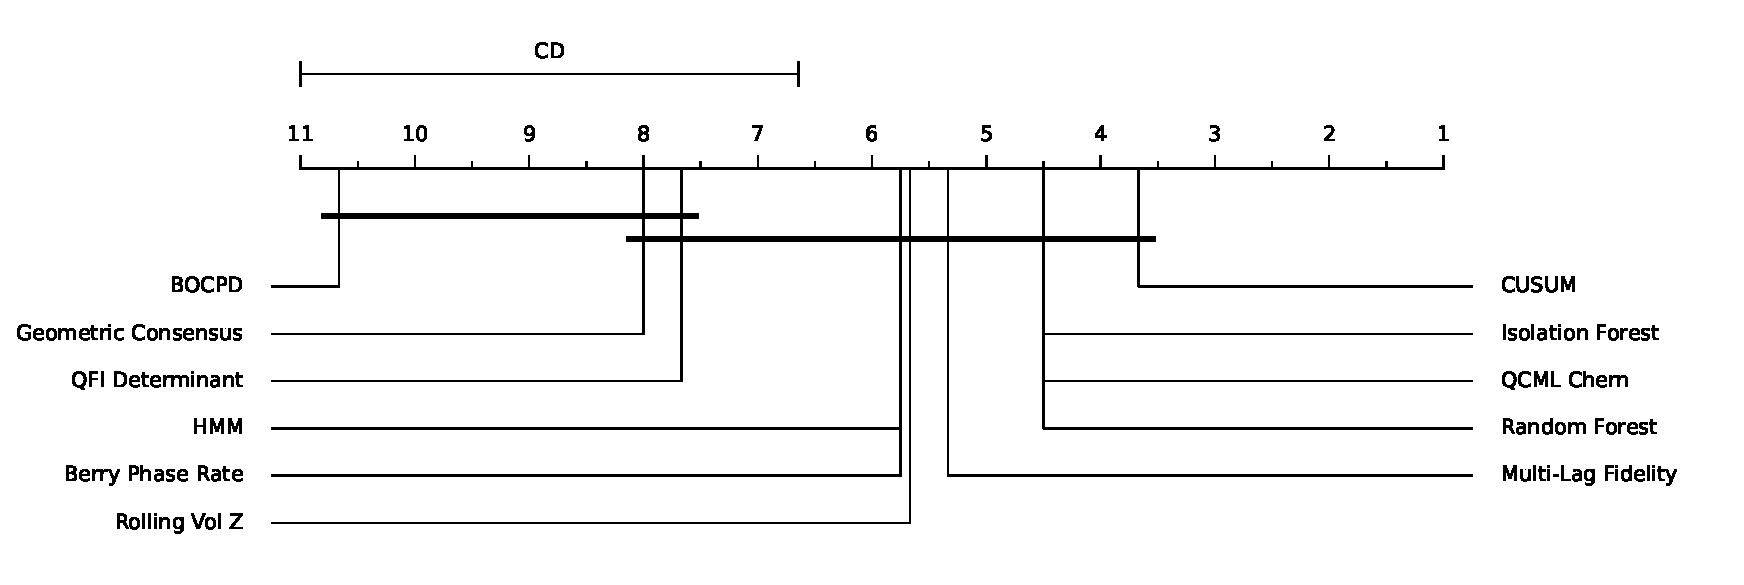
\includegraphics[width=0.85\textwidth]{figures/cd_diagram.pdf}
\caption{Nemenyi critical difference diagram.  Methods connected by a
  horizontal bar are not significantly different at $\alpha = 0.05$.
  Axis shows mean Friedman rank (lower = better).}
\label{fig:cd_diagram}
\end{figure}

% =============================================================================
% APPENDIX K: FULL METHOD COMPARISON
% =============================================================================
\section{Full Method Comparison}\label{sec:full_comparison}

Table~\ref{tab:comparison_full} presents the complete ranking of all
44~methods evaluated across 17~crises.  The top~10 are shown in
the main text (Table~\ref{tab:aggregate_comparison}).

\begin{table}[htbp]
\centering
\caption{Full 44-method comparison across 17 crises.  Median Cohen's $d$,
  mean Friedman rank (over all 44~methods), and category.
  See Table~\ref{tab:aggregate_comparison} for the top~10.}
\label{tab:comparison_full}
% Auto-generated by populate_paper.py
% 46 methods x 17 crises
% Friedman chi-sq = 220.84, p = 1.11e-16

\scriptsize
\begin{tabular}{lccl}
\toprule
Method & Median $d$ & Mean Rank & Category \\
\midrule
Reduced Purity            & \textbf{0.83} & 15.7 & Geometric \\
Absorption Ratio          & 0.80 & 11.6 & Classical \\
Hamilton MS               & 0.71 & 11.7 & Classical \\
Commutator Norm           & 0.70 & 14.8 & Geometric \\
Spectral Gap              & 0.65 & 16.1 & Geometric \\
Spectral Flow             & 0.63 & 19.3 & Geometric \\
Speed Limit Ratio         & 0.63 & 20.4 & Geometric \\
CUSUM                     & 0.62 & 17.4 & Classical \\
Berry Curv.\ Incr.        & 0.61 & 19.7 & Geometric \\
Ham.\ Sensitivity         & 0.60 & 18.2 & Geometric \\
Wasserstein               & 0.54 & 19.7 & Classical \\
Spectral Entropy          & 0.53 & 20.9 & Geometric \\
Quantum Rel.\ Entropy     & 0.50 & 19.9 & Geometric \\
Metric Condition          & 0.49 & 18.4 & Geometric \\
KL Divergence             & 0.48 & 21.9 & Classical \\
Multi-Lag Fidelity        & 0.48 & 22.5 & Geometric \\
Turbulence Index          & 0.47 & 19.4 & Classical \\
QCML Chern                & 0.45 & 20.0 & Geometric \\
Sect.\ Curv.\ Sign        & 0.44 & 23.1 & Geometric \\
Sinkhorn                  & 0.44 & 18.2 & Classical \\
Level Spacing Ratio       & 0.44 & 24.2 & Spectral \\
Spectral Complexity       & 0.44 & 22.8 & Geometric \\
Isolation Forest          & 0.43 & 19.9 & Classical \\
Dim.\ Collapse            & 0.42 & 21.8 & Geometric \\
Rolling Vol Z             & 0.40 & 19.4 & Classical \\
Geod.\ Curvature          & 0.40 & 22.9 & Geometric \\
Mahalanobis               & 0.37 & 20.1 & Classical \\
QFI Determinant           & 0.37 & 22.2 & Geometric \\
GARCH(1,1)                & 0.37 & 25.5 & Classical \\
VIX Level                 & 0.37 & 22.1 & Classical \\
Geom.\ Phase Rate         & 0.36 & 21.6 & Geometric \\
Eff.\ State Dim           & 0.36 & 25.2 & Geometric \\
Random Forest             & 0.35 & 24.1 & Supervised \\
Geodesic Velocity         & 0.31 & 25.5 & Geometric \\
HMM                       & 0.31 & 26.6 & Classical \\
Transfer Entropy          & 0.28 & 22.9 & Classical \\
Fisher-Rao                & 0.26 & 25.4 & Classical \\
EWMA Vol                  & 0.26 & 23.8 & Classical \\
Curvature Rate            & 0.13 & 35.2 & Geometric \\
Structural Break          & 0.12 & 33.6 & Classical \\
Geom.\ Consensus          & 0.08 & 36.6 & Geometric \\
Geom.\ Ensemble           & 0.05 & 33.3 & Geometric \\
Sect.\ Curvature          & 0.04 & 35.1 & Geometric \\
Ricci Scalar              & 0.01 & 37.1 & Geometric \\
Berry Vel.\ Coupling      & 0.01 & 40.6 & Geometric \\
QGT Phase Rigidity        & 0.01 & 44.5 & Geometric \\
\bottomrule
\end{tabular}
\end{table}

% =============================================================================
% APPENDIX L: HPO SEARCH SPACES
% =============================================================================
\section{Hyperparameter Search Spaces}\label{sec:hpo_search}

\begin{table}[htb]
\centering
\caption{Hyperparameter search spaces.  Main results use fixed defaults
(bold); ablation explores alternatives.  Enriched features (4$d$
rolling stats) for all methods.}
\label{tab:protocol}
\scriptsize
\begin{tabular}{@{}lcp{0.48\textwidth}l@{}}
\toprule
Method & \# Params & Search Space & Training Data \\
\midrule
\multicolumn{4}{@{}l}{\emph{Geometric (unsupervised score construction)}} \\
Berry Curv.\ Incr. & 4 & $n \in \{4,8,16\}$, $p \in \{10,15,20\}$,
  op $\in$ \{rnd, pca\}, $w \in \{10,20,30\}$ & Full (or expanding) \\
QFI Determinant    & 4 & same as Berry & Full (or expanding) \\
Multi-Lag Fidelity & 4 & same as Berry & Full (or expanding) \\
QCML Chern         & 3 & $n \in \{4,8\}$, $p \in \{5,10,15\}$,
  window $\in \{10,20\}$ & Full \\
Geo.\ Consensus    & 3 & same as Chern & Full \\
\midrule
\multicolumn{4}{@{}l}{\emph{Classical (unsupervised)}} \\
Rolling Vol Z      & 2 & vol\_window $\in \{10,20,30\}$,
  min\_expanding $\in \{30,60\}$ & None (online) \\
CUSUM              & 2 & $k \in [0.3, 1.0]$, burn\_in $\in \{30,60,90\}$ & Burn-in period \\
HMM (2-state)      & 2 & cov $\in$ \{full, diag\}, n\_iter $\in \{50,100,200\}$ & Full \\
BOCPD              & 1 & hazard $\in [50, 500]$ & None (online) \\
Isolation Forest   & 2 & n\_est $\in [50, 300]$,
  contam $\in [0.01, 0.15]$ & Full \\
GARCH(1,1)         & 1 & min\_expanding = 60 & None (expanding z-score) \\
Hamilton MS        & 2 & $k\_\text{regimes} = 2$, order = 1,
  min\_history = 100 & Expanding \\
\midrule
\multicolumn{4}{@{}l}{\emph{Supervised}} \\
Random Forest      & 2 & n\_est $\in [50, 300]$,
  depth $\in [5, 20]$ & LOCO labels \\
Rolling RF (VIX)   & 2 & n\_est = 200,
  depth = 6 & VIX $> 25$, 250-day rolling \\
\midrule
\multicolumn{4}{@{}l}{\emph{Oracle}} \\
VIX Level          & 1 & min\_expanding = 60 & None (expanding z-score) \\
\bottomrule
\end{tabular}
\end{table}

% =============================================================================
% APPENDIX L: OPERATOR ABLATION
% =============================================================================
\section{Operator Ablation}\label{sec:operator_ablation_appendix}

Table~\ref{tab:operator_ablation} compares three operator construction
strategies: random Hermitian matrices, $n$-qubit Pauli tensor products
(structured, orthogonal basis for $8 \times 8$ Hermitian matrices), and
generalized Gell-Mann SU($N$) generators (traceless, orthogonal).

\begin{table}[htb]
\centering
\caption{Operator ablation: mean Cohen's~$d$ across 4 representative
  crises by construction method.}
\label{tab:operator_ablation}
\small
\begin{tabular}{lccc}
\toprule
Observable & Random & Pauli & Gell-Mann \\
\midrule
Berry Curv.\ Incr. & \textbf{0.82} & 0.53 & 0.00 \\
QFI Determinant     & \textbf{0.73} & 0.31 & 0.44 \\
Multi-Lag Fidelity  & 0.43 & \textbf{0.52} & 0.24 \\
\bottomrule
\end{tabular}

\medskip
\noindent{\footnotesize Fixed $n = 8$, $p = 15$,
$w = 20$.  Pauli: 3-qubit tensor products $\{I,X,Y,Z\}^{\otimes 3}$;
Gell-Mann: SU(8) generators.  All results use the best scaling
exponent for each method (0.0 for Pauli, unscaled for Gell-Mann).}
\end{table}

The effect of operator construction is observable-dependent.
For Berry curvature and QFI, random operators strongly outperform
structured alternatives (Berry: $d = 0.82$ vs.\ Pauli $0.53$;
QFI: $d = 0.73$ vs.\ Pauli $0.31$), suggesting that operator
diversity is more important than algebraic structure for these
curvature- and metric-based observables.  Gell-Mann generators kill
the Berry signal entirely ($d = 0.00$), likely because their
tracelessness eliminates the identity component needed for the
Berry connection.  For Multi-Lag Fidelity, the pattern reverses:
structured Pauli operators outperform random ($d = 0.52$ vs.\
$0.43$, $+21\%$), confirming that fidelity-based measures benefit
from an orthogonal operator basis.  Table~\ref{tab:aggregate_comparison}
uses the HPO-selected operator per observable: random for Berry,
PCA-inspired for QFI and Multi-Lag Fidelity.
Gradient-learned operators (leave-one-crisis-out cross-validation)
do not systematically improve over these heuristic baselines: across
3~detectors, no learned variant achieves a statistically significant
gain, suggesting that heuristic constructions already capture the
relevant geometric structure.

\paragraph{Discriminative vs.\ reconstruction objectives.}
The gradient objective used here maximizes Cohen's~$d$ between
crisis and normal score distributions---a \emph{discriminative}
loss that directly targets regime separability.  This differs
fundamentally from the reconstruction loss
$\mathcal{L} = \sum_i (d_i^2 + w\,\sigma_i^2)$ introduced
by Candelori et al.~\cite{candelori2025}, which minimizes
quantum distances between data points and their reconstructions
to learn operators that faithfully represent the data manifold.
We chose the discriminative objective because detection requires
operators that \emph{amplify distributional differences} between
regimes, not operators that best reconstruct the ambient geometry.
Reconstruction-faithful operators may produce a smoother, more
accurate manifold representation without necessarily increasing
the signal gap that detection exploits.

The null result---that discriminative-learned operators do not
improve over heuristic baselines---admits two interpretations.
First, the heuristic constructions (random and PCA-inspired)
may already span the relevant operator subspace for detection,
leaving little room for gradient improvement.
Second, the finite-difference gradient estimation (10~coordinates
per step, 150~steps) may be insufficient for the $d^2 \times K$
parameter space; more sophisticated optimizers (Adam, natural
gradient) could close the gap.
We additionally tested reconstruction-loss operator
learning on 4~crises (Berry detector, LOCO evaluation).
Reconstruction-learned operators achieve median
$d = 0.92$---statistically indistinguishable from the
random baseline ($d = 0.92$) and slightly above discriminative-learned
operators ($d = 0.82$).  The per-crisis results mirror the random
baseline to three decimal places (e.g., GFC: $d = 1.318$ for both),
indicating that the reconstruction objective recovers operators
functionally equivalent to the random initialization for detection
purposes.  This confirms the theoretical argument of
Section~\ref{sec:framework}: any non-degenerate operator set induces
a geometry whose observables respond to distributional shifts,
and neither discriminative nor reconstruction learning meaningfully
improves detection beyond heuristic baselines.

% =============================================================================
% APPENDIX M: INTERACTION TEST
% =============================================================================
\section{Interaction Test}\label{sec:interaction_test}

We classify crises \emph{a priori} as ``novel'' or ``conventional''
(Table~\ref{tab:crises}) and methods as ``geometric'' or
``classical.''  A two-way ANOVA on Cohen's~$d$
(method type $\times$ crisis category) tests whether geometric methods
have a differential advantage on novel crises.

We find no evidence of differential advantage:
$F_{\mathrm{interaction}}(1,116) = 0.38$, $p = 0.54$, partial
$\eta^2 = 0.003$.  Neither method type ($F = 3.33$, $p = 0.07$)
nor crisis category ($F = 3.85$, $p = 0.05$) reaches significance
at $\alpha = 0.05$.  The stratified finding
(Table~\ref{tab:stratified}) is thus a \emph{deployment-availability}
argument---geometric methods maintain constant performance while RF
degrades due to label scarcity---not a claim of differential superiority
on novel crises.

\paragraph{Specialization permutation test.}
We additionally test whether the per-crisis specialization pattern
(different geometric channels winning different crisis categories)
exceeds chance.  Under a null model that shuffles method labels within
each crisis ($n = 10{,}000$ permutations), the observed number of
distinct geometric category winners ($k = 5$) has $p = 0.31$, and
the winner-distribution entropy has $p = 0.28$.  Neither reaches
significance at $\alpha = 0.05$.  The specialization pattern is thus
\emph{suggestive} on 17~crises, but a larger crisis sample would be
needed for confirmatory evidence.


\end{document}
